\subsection{Repositorio}

Los notebooks \texttt{.ipynb} así como los demás archivos de la práctica
se encuentran en el siguiente repositorio de GitHub:
\hyperlink{P4}{\textcolor{iimasorange}{https://github.com/Garp02/Reconocimiento-Patrones/tree/main/P4}}

De los cuatro conjuntos propuestos se eligieron dos: \textbf{Breast Cancer
    Wisconsin Diagnostic} y \textbf{Heart Disease}. Ambos son problemas de
clasificación binaria en el dominio biomédico, pero presentan retos
complementarios que permiten contrastar el comportamiento de los tres
clasificadores: el primero es prácticamente ``ideal'' (sin faltantes, con
30 características numéricas y clases bien separadas en el espacio de
entrada), mientras que el segundo concentra las dificultades típicas de un
conjunto clínico real (faltantes masivos, mezcla de variables continuas y
categóricas codificadas, y separación de clases mucho menos limpia).

Como esquema común para los dos conjuntos se siguió el flujo: carga
$\to$ exploración $\to$ preprocesamiento $\to$ partición $70/30$
estratificada $\to$ SMOTE sobre \textit{train} $\to$ PCA (\textit{mle},
$95\%$ de varianza y proyección 2D) $\to$ \textit{grid search} con CV de
5 \textit{folds} para KNN, árbol de decisión y SVM $\to$ evaluación final
sobre el conjunto de prueba. La semilla \texttt{random\_state = 43} se usó
en todos los componentes estocásticos para garantizar reproducibilidad.

\needspace{4\baselineskip}

\subsection{Conjunto de datos: Breast Cancer Wisconsin Diagnostic}

\subsubsection*{Carga y exploración}

El conjunto \textbf{Breast Cancer Wisconsin Diagnostic} contiene
\textbf{569 muestras} y \textbf{30 características numéricas} obtenidas a
partir de imágenes digitalizadas de aspiraciones con aguja fina (FNA) de
masas mamarias. Las características se agrupan en tres bloques de diez
variables que describen el mismo conjunto de propiedades morfológicas
(radio, textura, perímetro, área, suavidad, compacidad, concavidad, puntos
cóncavos, simetría y dimensión fractal) en tres escalas estadísticas:
\textit{mean} (promedio del núcleo celular), \textit{se} (error estándar)
y \textit{worst} (peor caso, definido como la media de los tres valores
más extremos). La variable objetivo \texttt{diagnosis} toma los valores
\texttt{B} (benigno, 357 casos) y \texttt{M} (maligno, 212 casos), lo que
arroja un \textit{ratio} mayoría/minoría de $1{:}0{.}59$ ---ligeramente
desbalanceado, pero lejos del umbral que suele requerir intervención
agresiva.

El perfilamiento exploratorio con \texttt{ydata\_profiling} se ejecutó
únicamente sobre las diez variables \textit{mean} para no inflar el tiempo
de generación del reporte. La revisión confirmó la \textbf{ausencia
    completa de valores faltantes} en todo el conjunto y verificó que las
escalas de las características difieren considerablemente: por ejemplo,
\texttt{area\_worst} ronda valores entre 200 y 4254, mientras que
\texttt{smoothness\_mean} se mueve entre $0.05$ y $0.16$. Esta diferencia
de varios órdenes de magnitud justifica plenamente el escalado posterior.

\subsubsection*{Detección de \textit{outliers} con IQR}

Se aplicó el criterio intercuartílico ($Q_1 - 1.5 \cdot IQR$ y
$Q_3 + 1.5 \cdot IQR$) sobre las 30 características numéricas. La variable
\texttt{area\_se} concentra el mayor número de valores extremos (65, el
$11.4\%$), seguida por \texttt{radius\_se} y \texttt{perimeter\_se}
(ambas con 38, el $6.7\%$). En total, \textbf{171 de las 569 filas}
contienen al menos un \textit{outlier} bajo IQR, una proporción
significativa que en otro contexto podría motivar su eliminación. En este
caso no se removieron, por dos razones: muchos valores extremos
corresponden a tumores efectivamente agresivos (información biológica
legítima, no errores de medición) y, al aplicar después un escalado
\textit{z-score}, su impacto sobre los modelos se atenúa.

Los \textit{boxplots} de las Figura~\ref{fig:cancer-boxplots-mean},
\ref{fig:cancer-boxplots-se} y \ref{fig:cancer-boxplots-worst} comparan las
distribuciones \textit{Benigno} vs \textit{Maligno} para los tres grupos
de variables. Se aprecia visualmente que los tumores malignos tienden a
producir valores sistemáticamente mayores en casi todas las características
\textit{mean} y \textit{worst}, mientras que las variables \textit{se}
muestran solapamiento más marcado.

\begin{figure}[H]
    \centering
    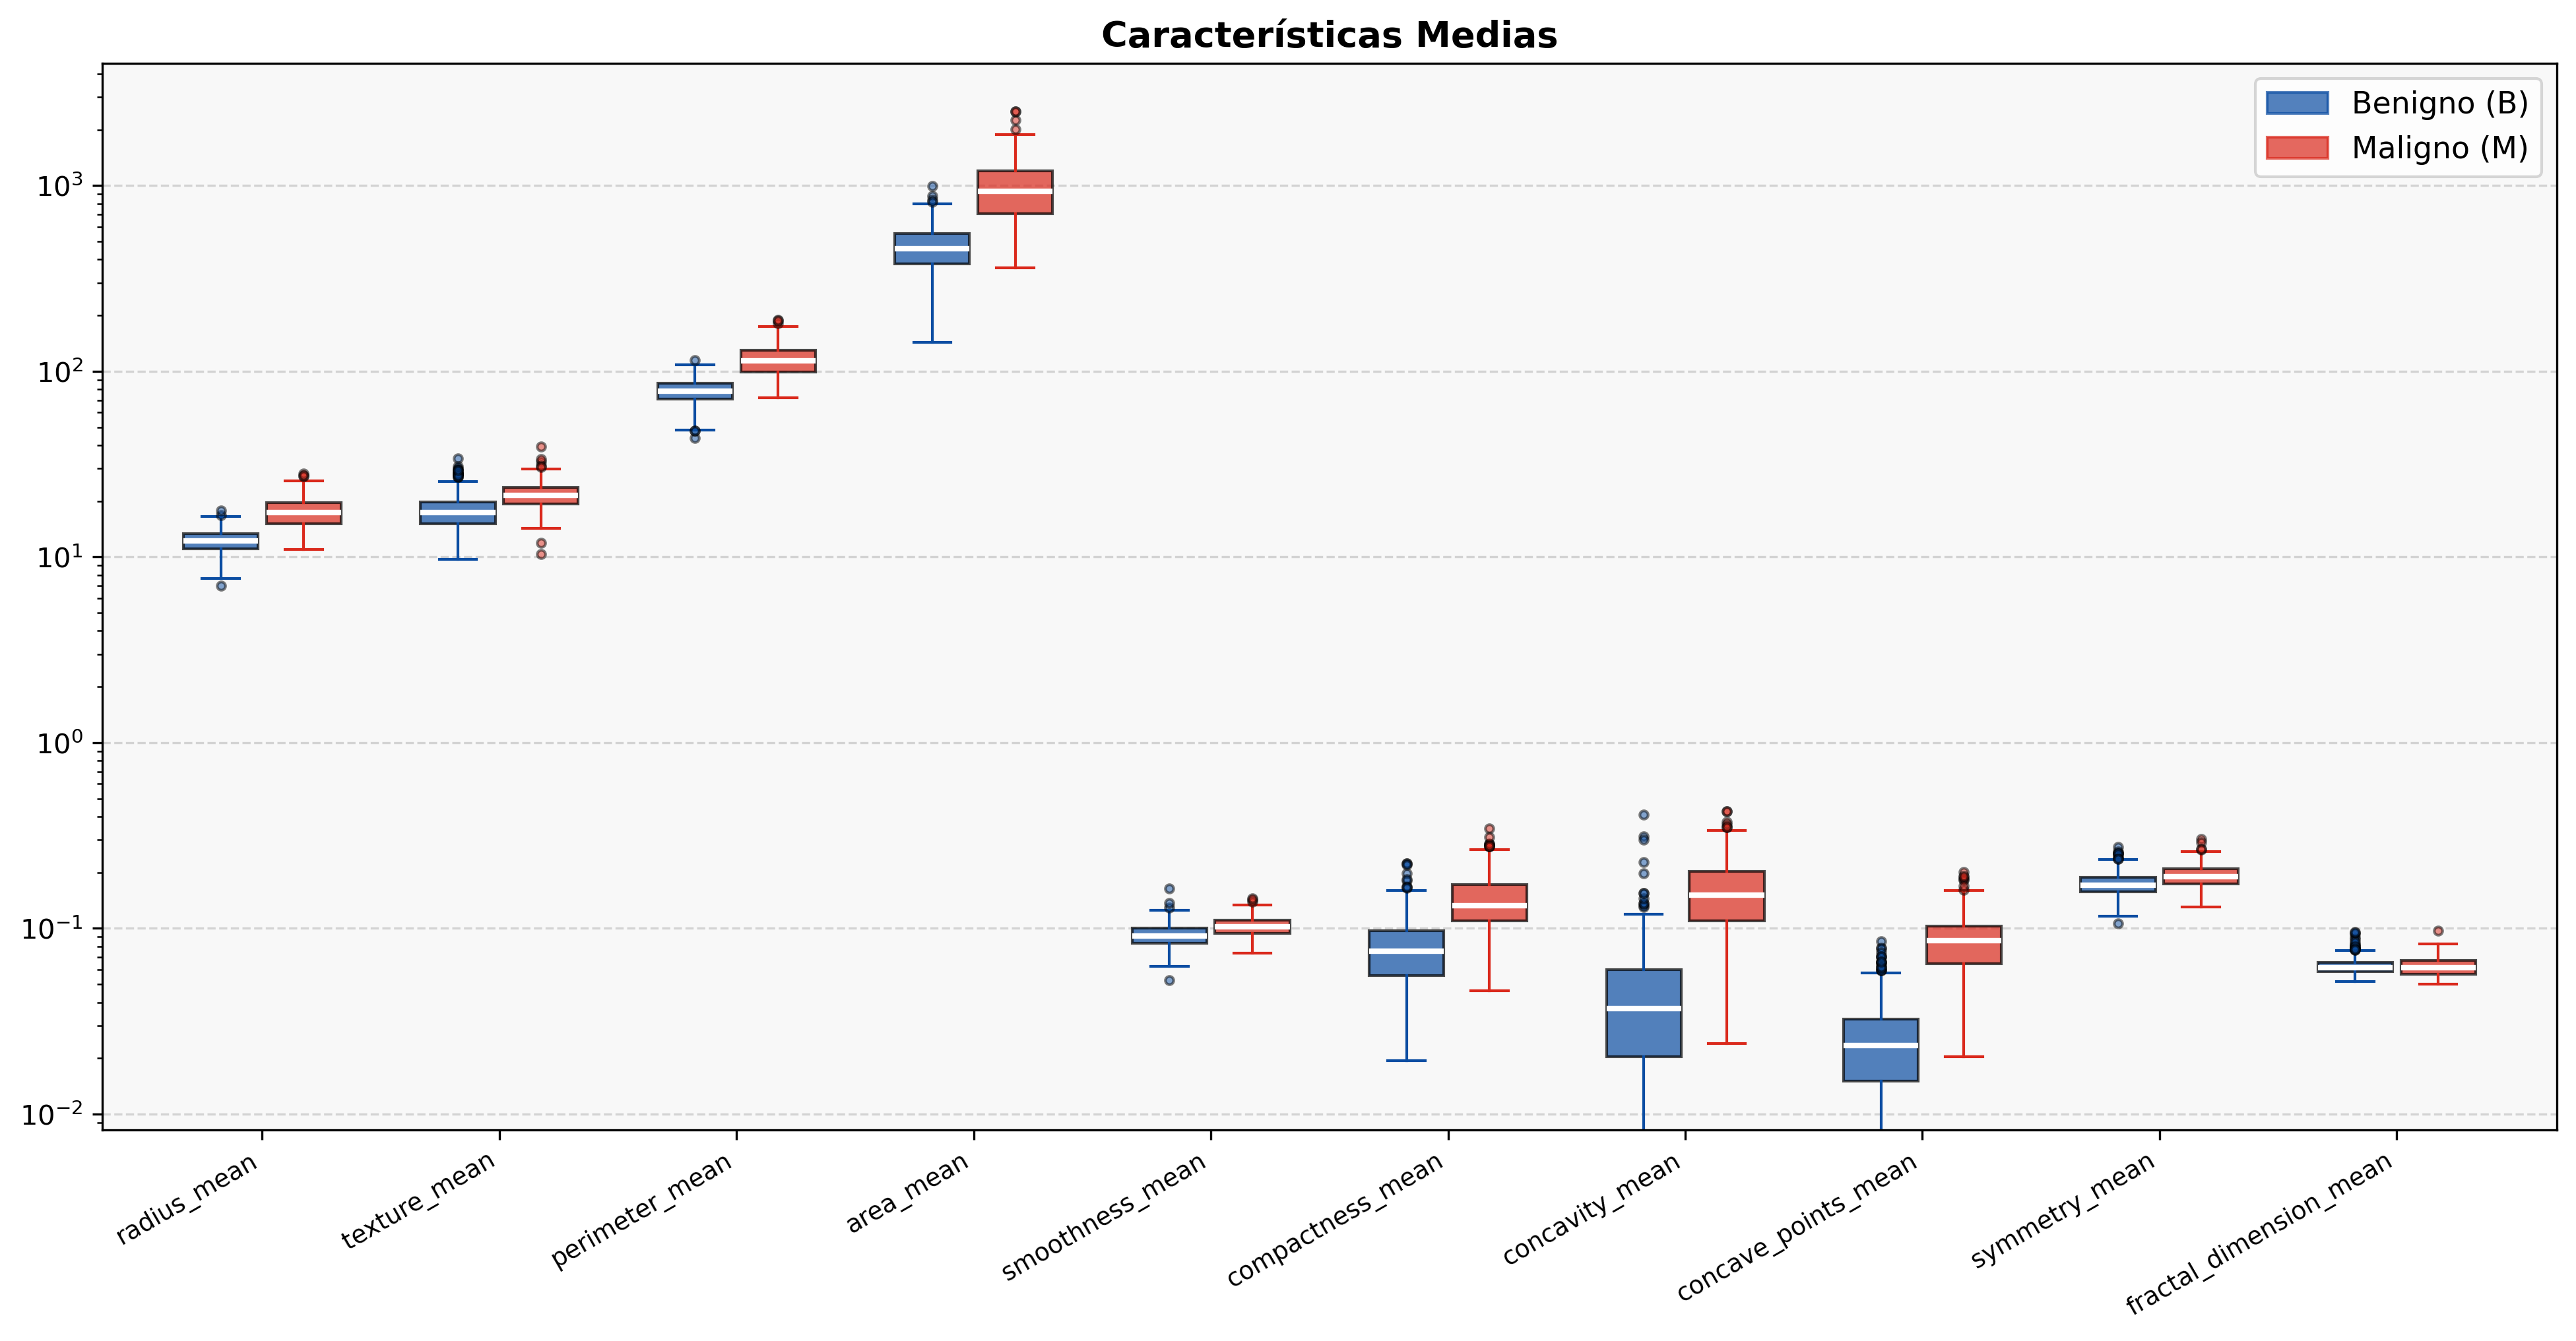
\includegraphics[width=0.95\textwidth]{Img/01_boxplot_cancer_Características_Medias.png}
    \caption{\textit{Boxplots} comparativos del grupo de características \textit{mean}
        del conjunto Cancer. Escala logarítmica.}
    \label{fig:cancer-boxplots-mean}
\end{figure}

\begin{figure}[H]
    \centering
    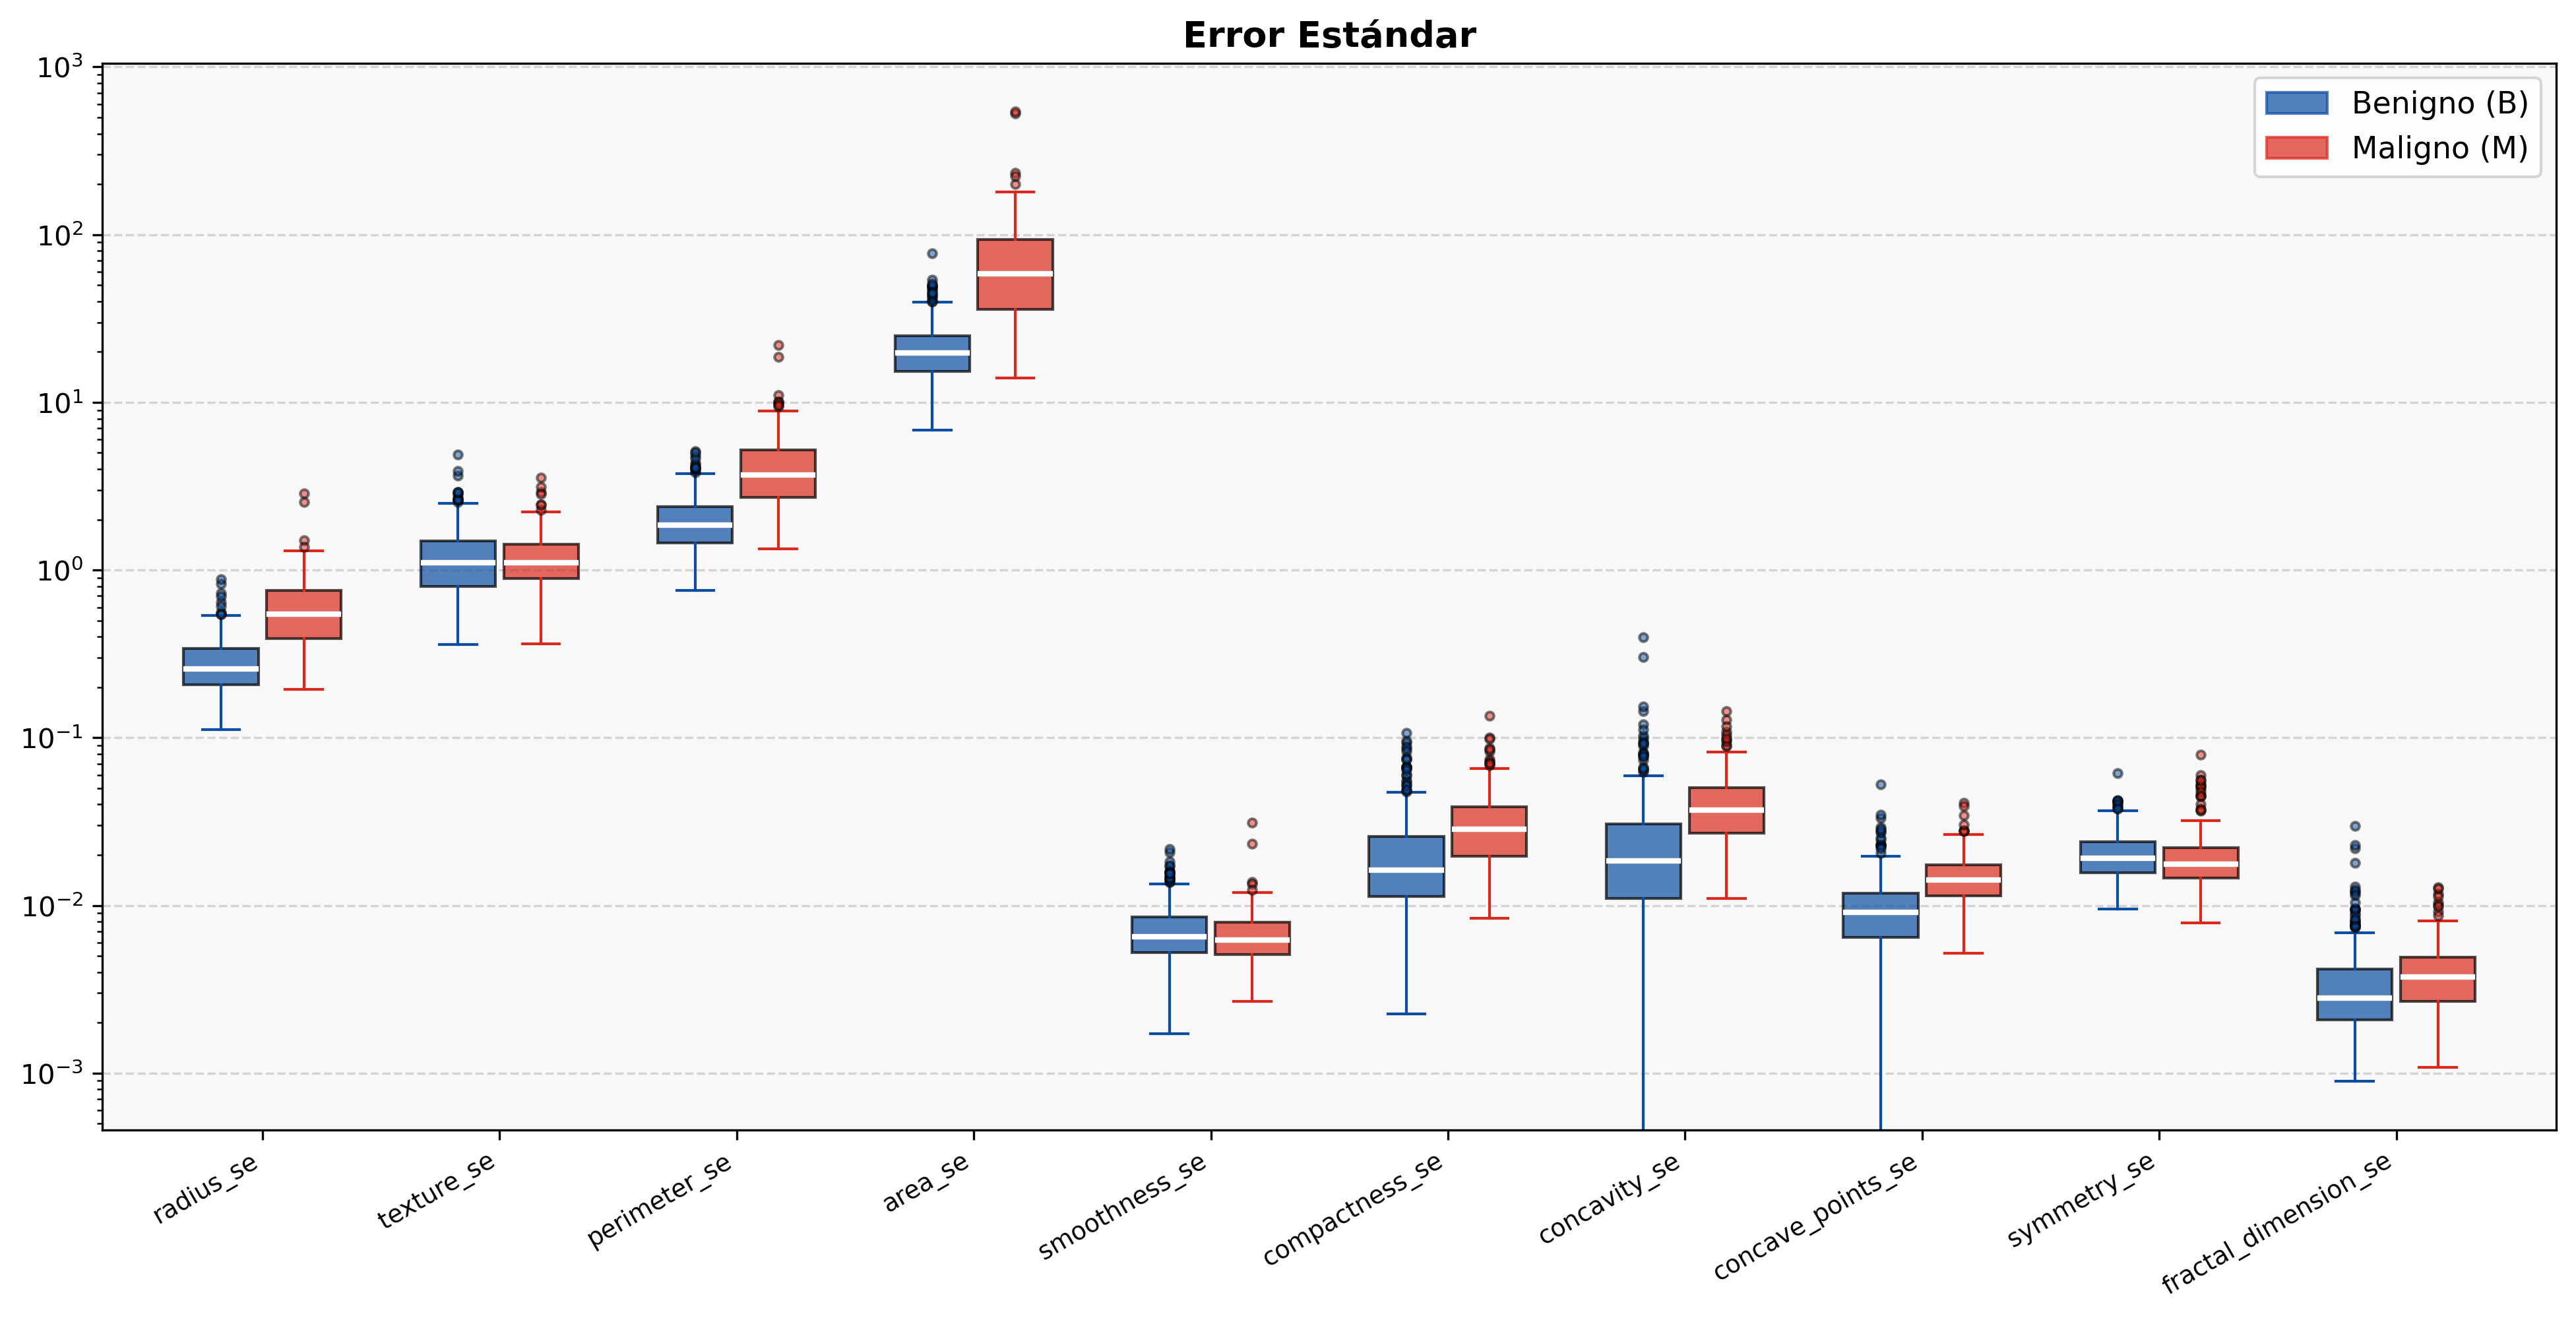
\includegraphics[width=0.95\textwidth]{Img/01_boxplot_cancer_Error_Estándar.png}
    \caption{\textit{Boxplots} comparativos del grupo de características \textit{se}
        del conjunto Cancer. Escala logarítmica.}
    \label{fig:cancer-boxplots-se}
\end{figure}

\begin{figure}[H]
    \centering
    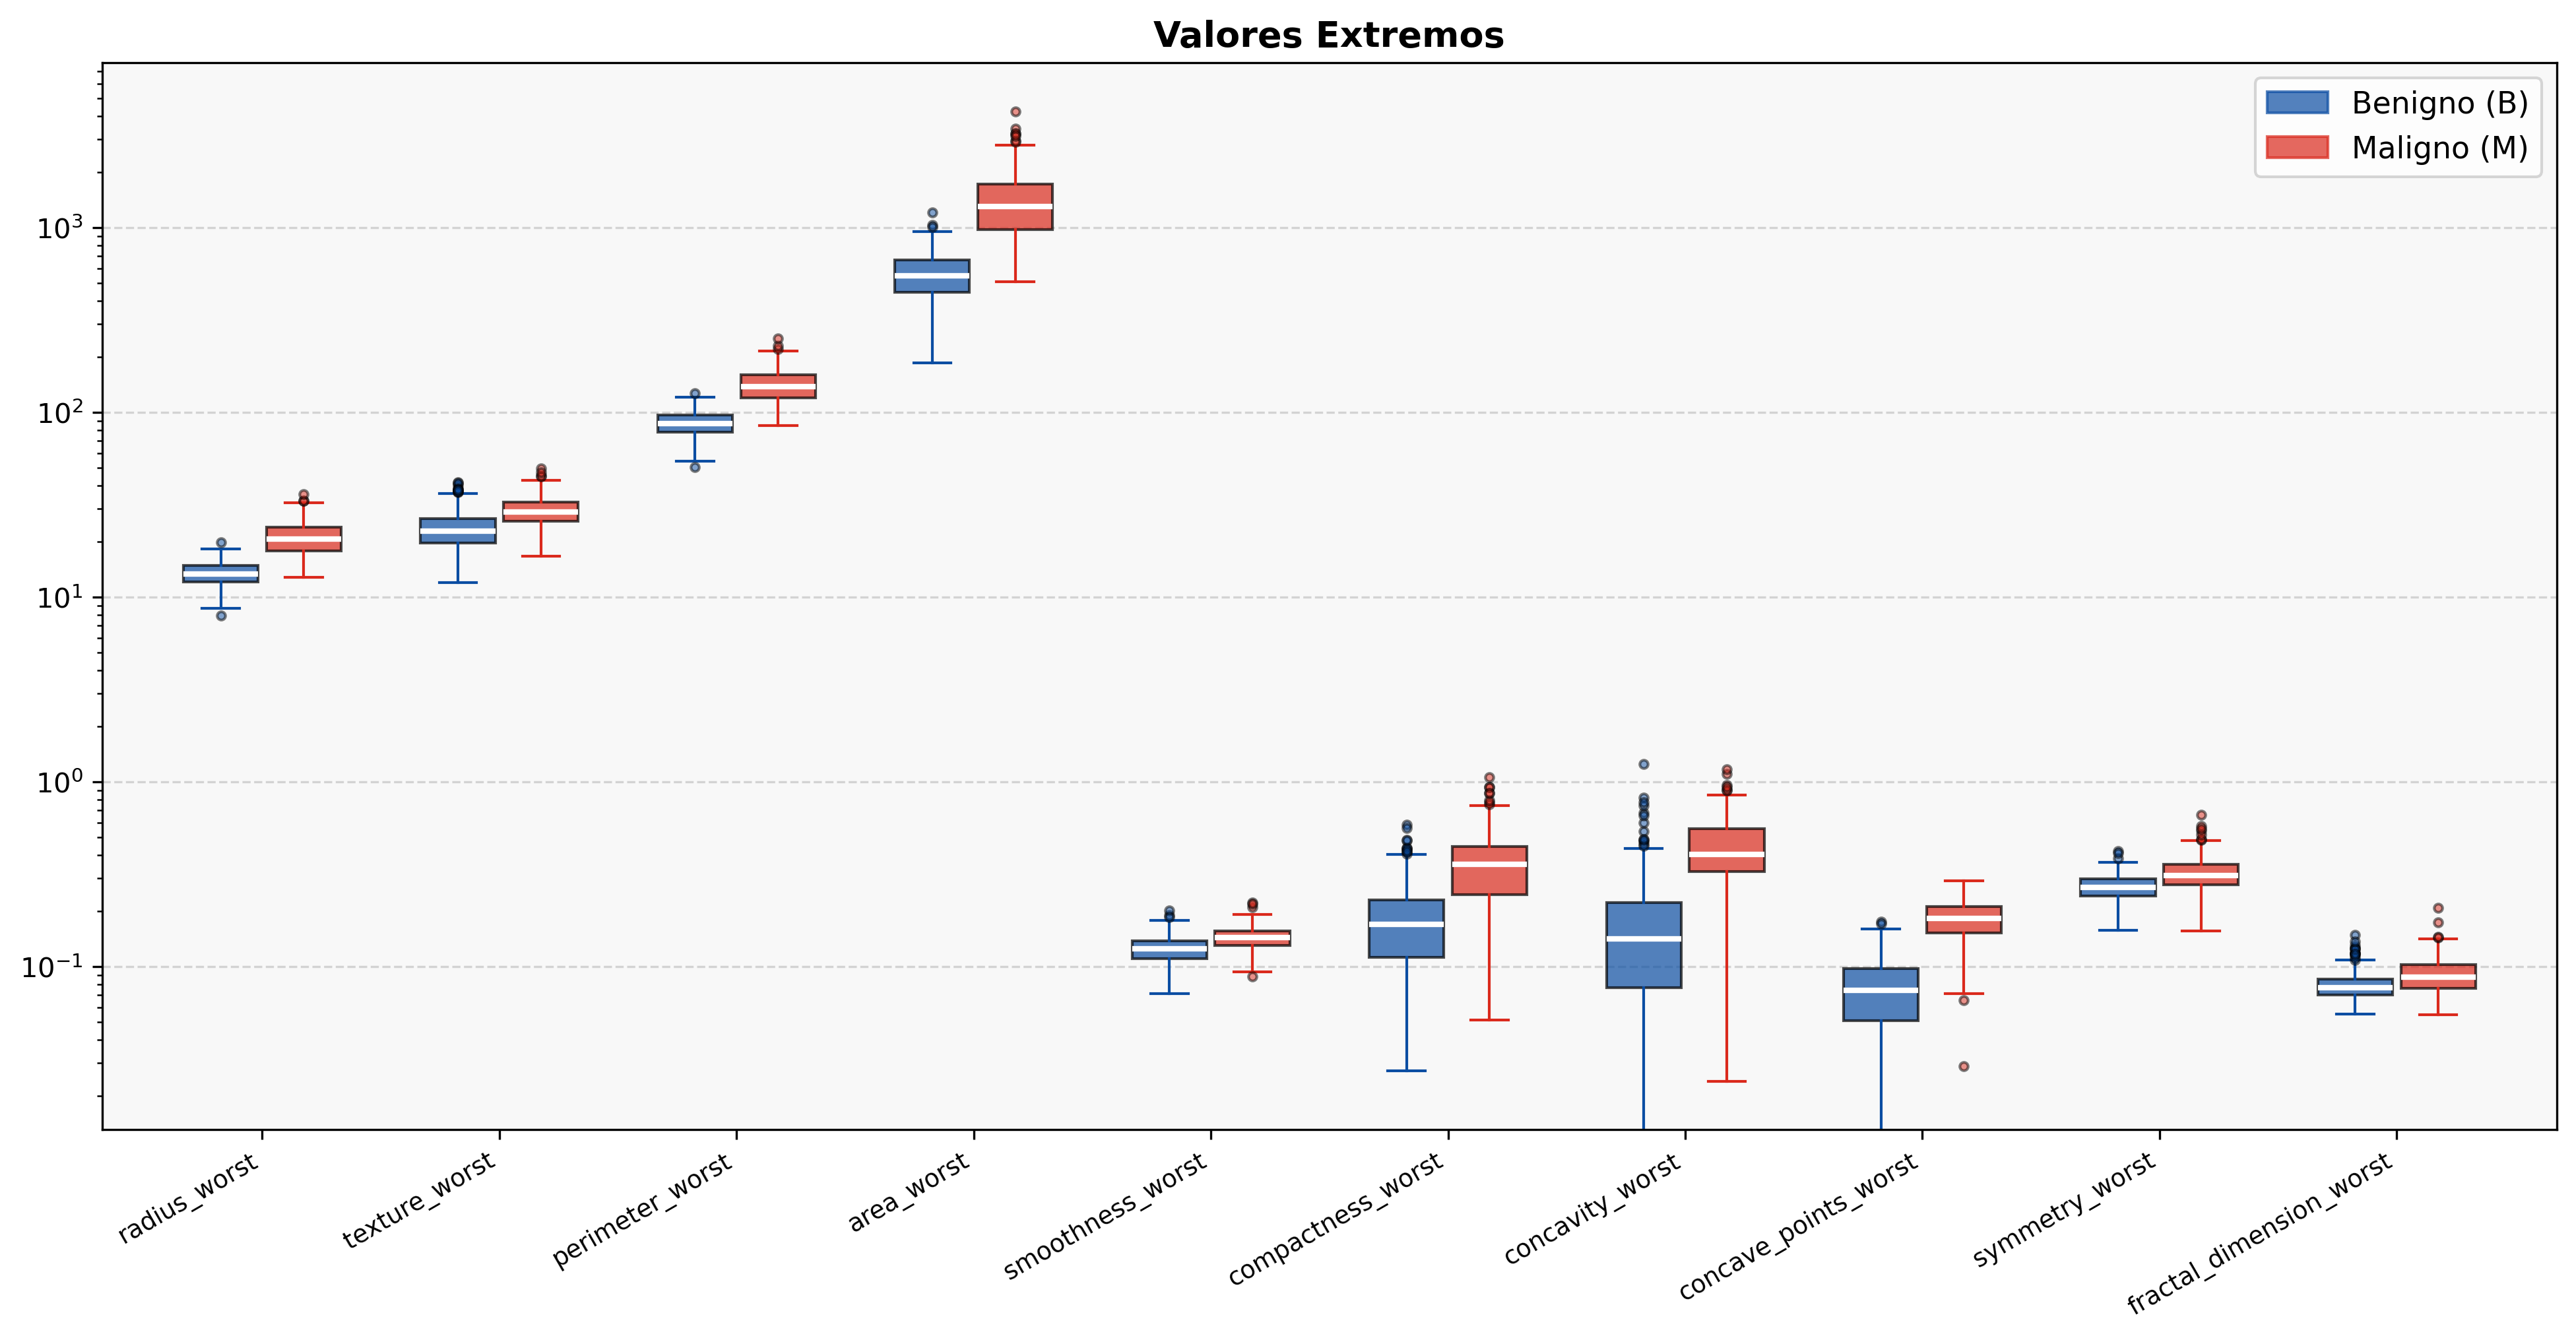
\includegraphics[width=0.95\textwidth]{Img/01_boxplot_cancer_Valores_Extremos.png}
    \caption{\textit{Boxplots} comparativos del grupo de características \textit{worst}
        del conjunto Cancer. Escala logarítmica.}
    \label{fig:cancer-boxplots-worst}
\end{figure}

\subsubsection*{Preprocesamiento, partición y SMOTE}

Las 30 variables numéricas se estandarizaron con \texttt{StandardScaler}
y se separaron en $70\%$ entrenamiento ($n=398$) y $30\%$ prueba ($n=171$)
mediante \texttt{train\_test\_split} con \texttt{stratify=y} y
\texttt{random\_state=43}. Aunque el desbalance original ($0.59$) es
moderado, se aplicó \textbf{SMOTE} sobre el conjunto de entrenamiento por
fidelidad al enunciado de la práctica. Esto elevó el número de muestras
malignas de 148 a 250, igualando ambas clases y produciendo un conjunto
balanceado de 500 muestras
(Figura~\ref{fig:cancer-smote}).

\begin{figure}[H]
    \centering
    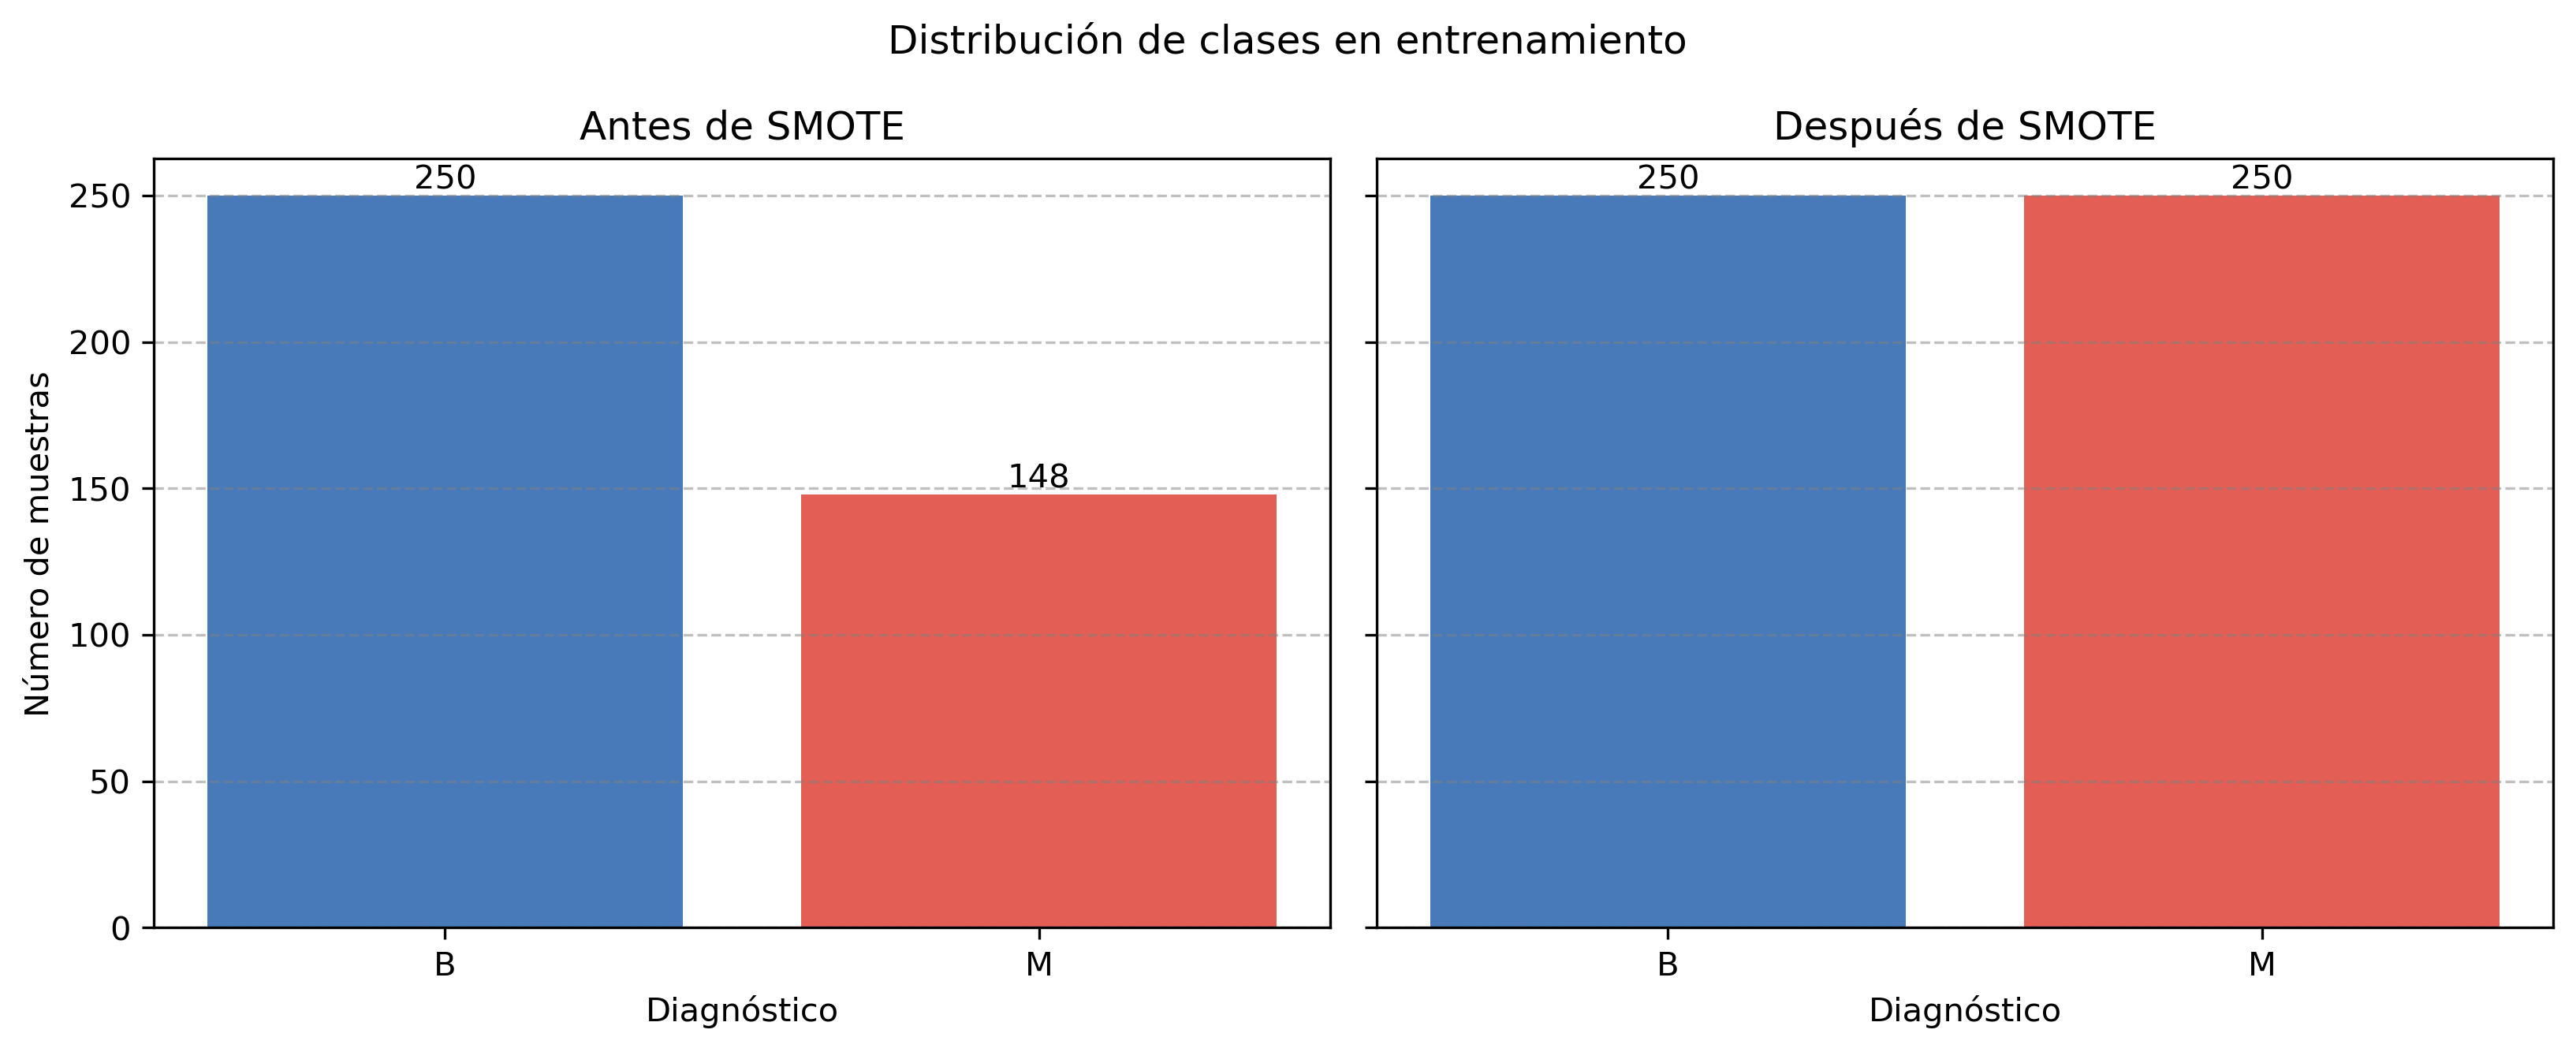
\includegraphics[width=0.85\textwidth]{Img/02_distribucion_smote_cancer.png}
    \caption{Distribución de clases en el conjunto de entrenamiento de
        Cancer, antes y después de aplicar SMOTE.}
    \label{fig:cancer-smote}
\end{figure}

\subsubsection*{Reducción de dimensionalidad con PCA}

Se compararon tres configuraciones de PCA: estimación automática con
\textit{Minka's Maximum Likelihood Estimation} (\texttt{n\_components =
    'mle'}), umbral de varianza acumulada del $95\%$ y proyección a 2
componentes para visualización. El método MLE seleccionó \textbf{29
    componentes} (esencialmente conserva todo el espacio original, lo que
indica que prácticamente todas las direcciones aportan información
estadísticamente significativa); el umbral del $95\%$ se alcanza con tan
solo \textbf{10 componentes}; y las dos primeras componentes capturan ya
una fracción considerable de la varianza
(Figura~\ref{fig:cancer-var-mle}).

\begin{figure}[H]
    \centering
    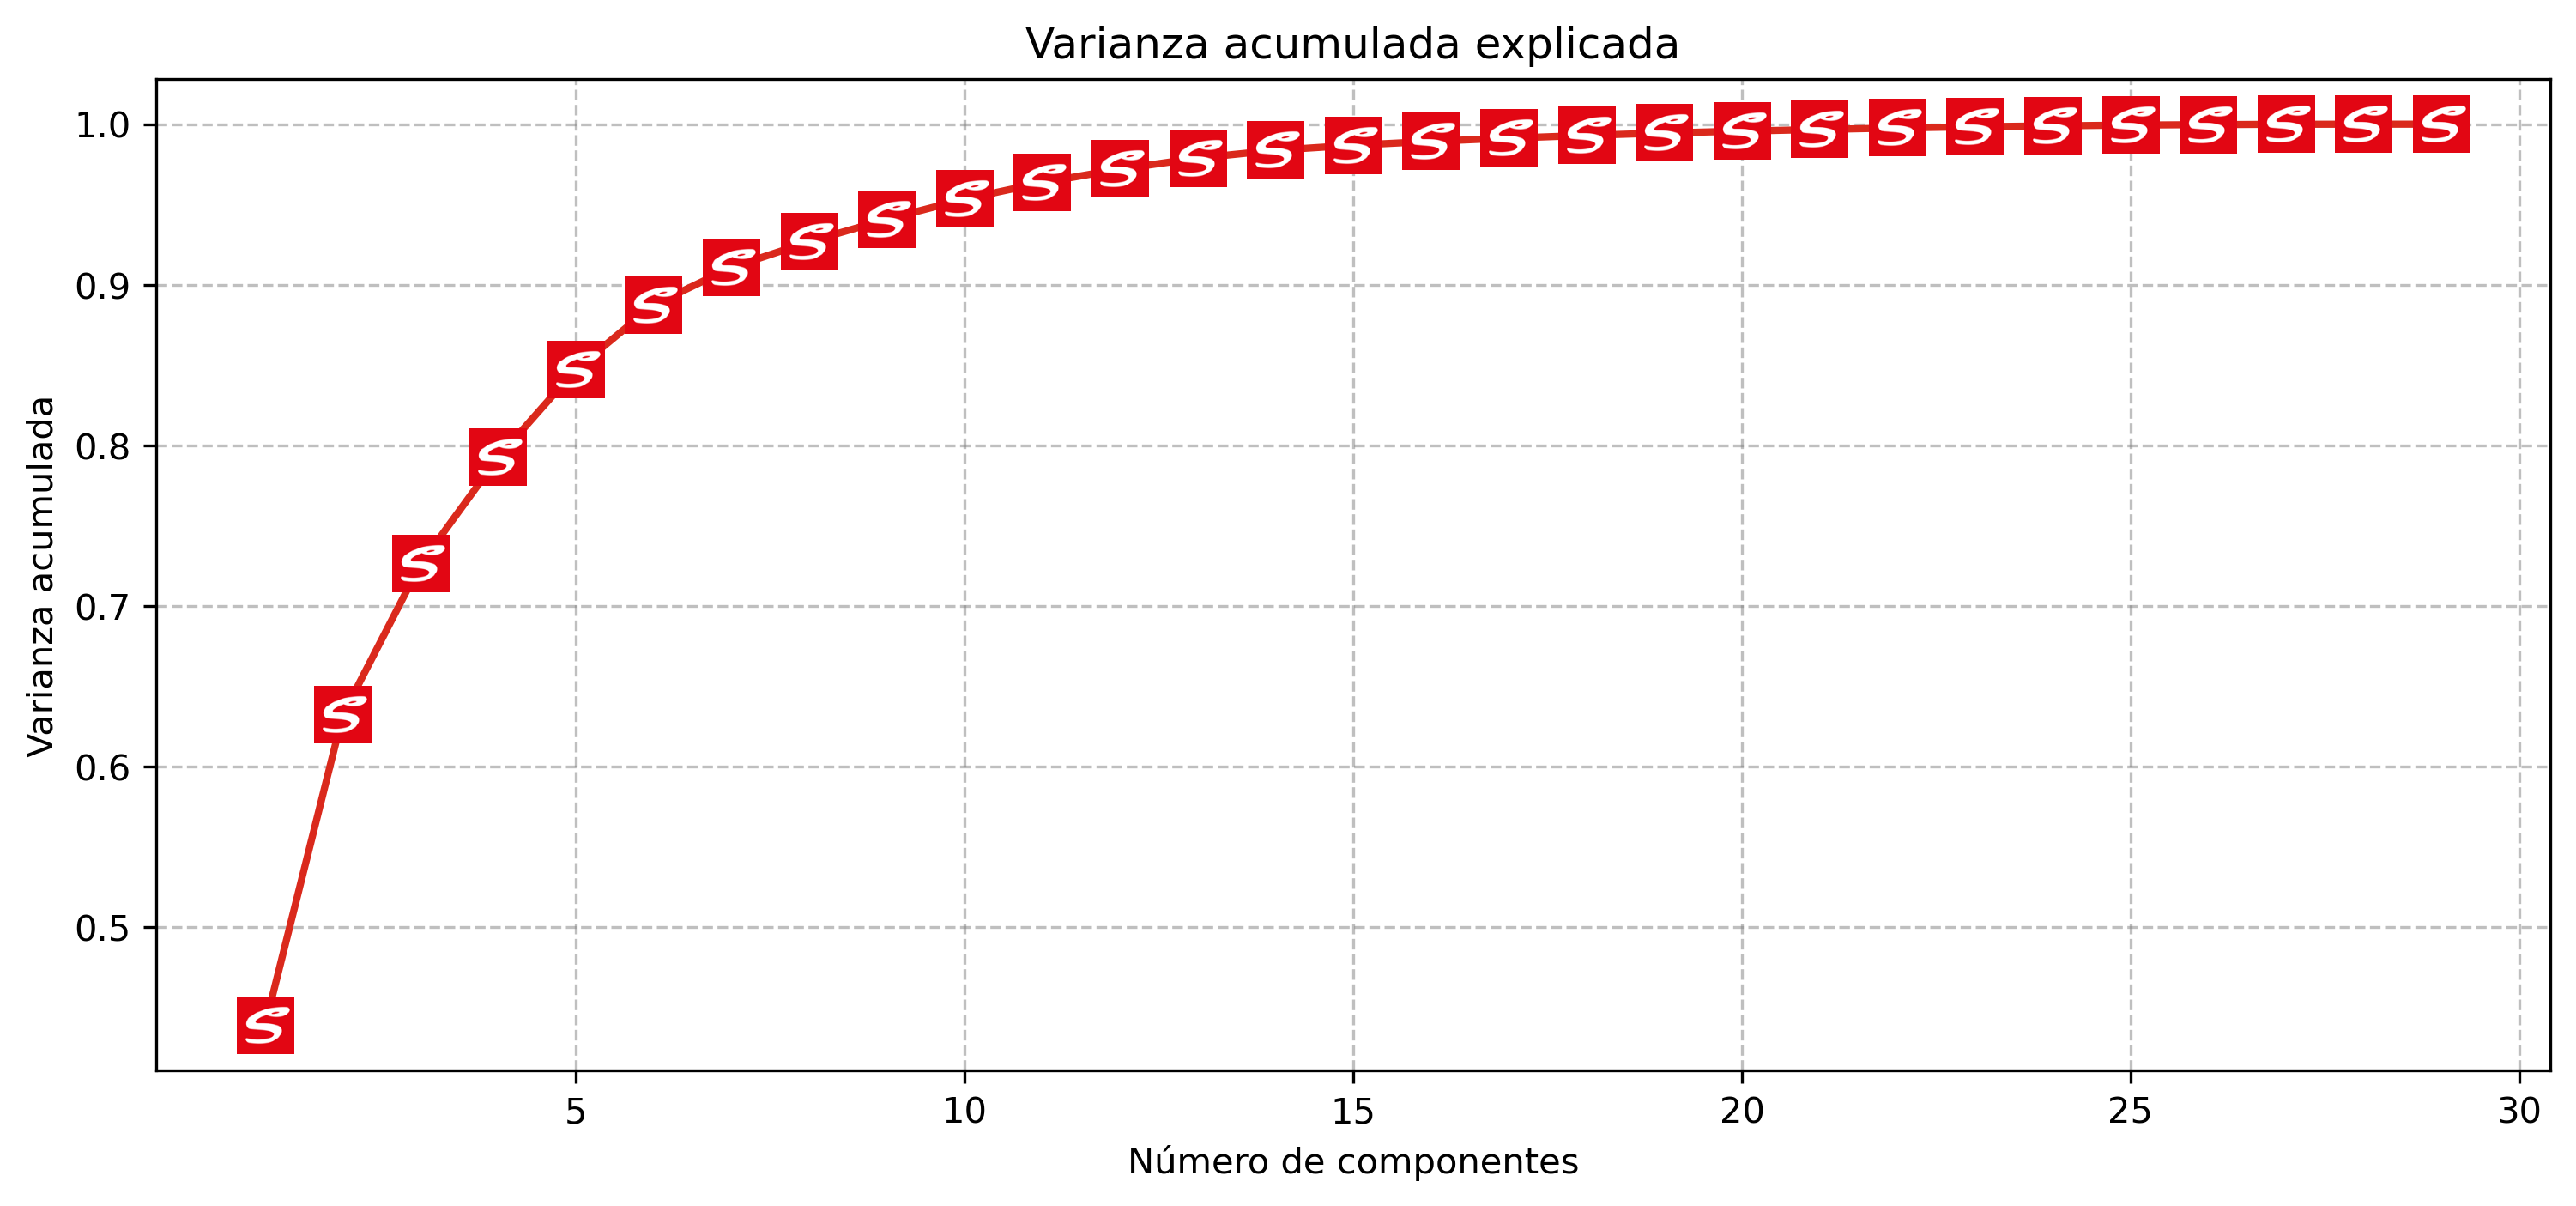
\includegraphics[width=0.95\textwidth]{Img/03_varianza_acumulada_pesea_mle.png}
    \caption{Varianza acumulada para PCA con \textit{Minka's MLE} sobre
        Cancer. Los 29 componentes seleccionados absorben casi la totalidad
        de la varianza.}
    \label{fig:cancer-var-mle}
\end{figure}

\begin{figure}[H]
    \centering
    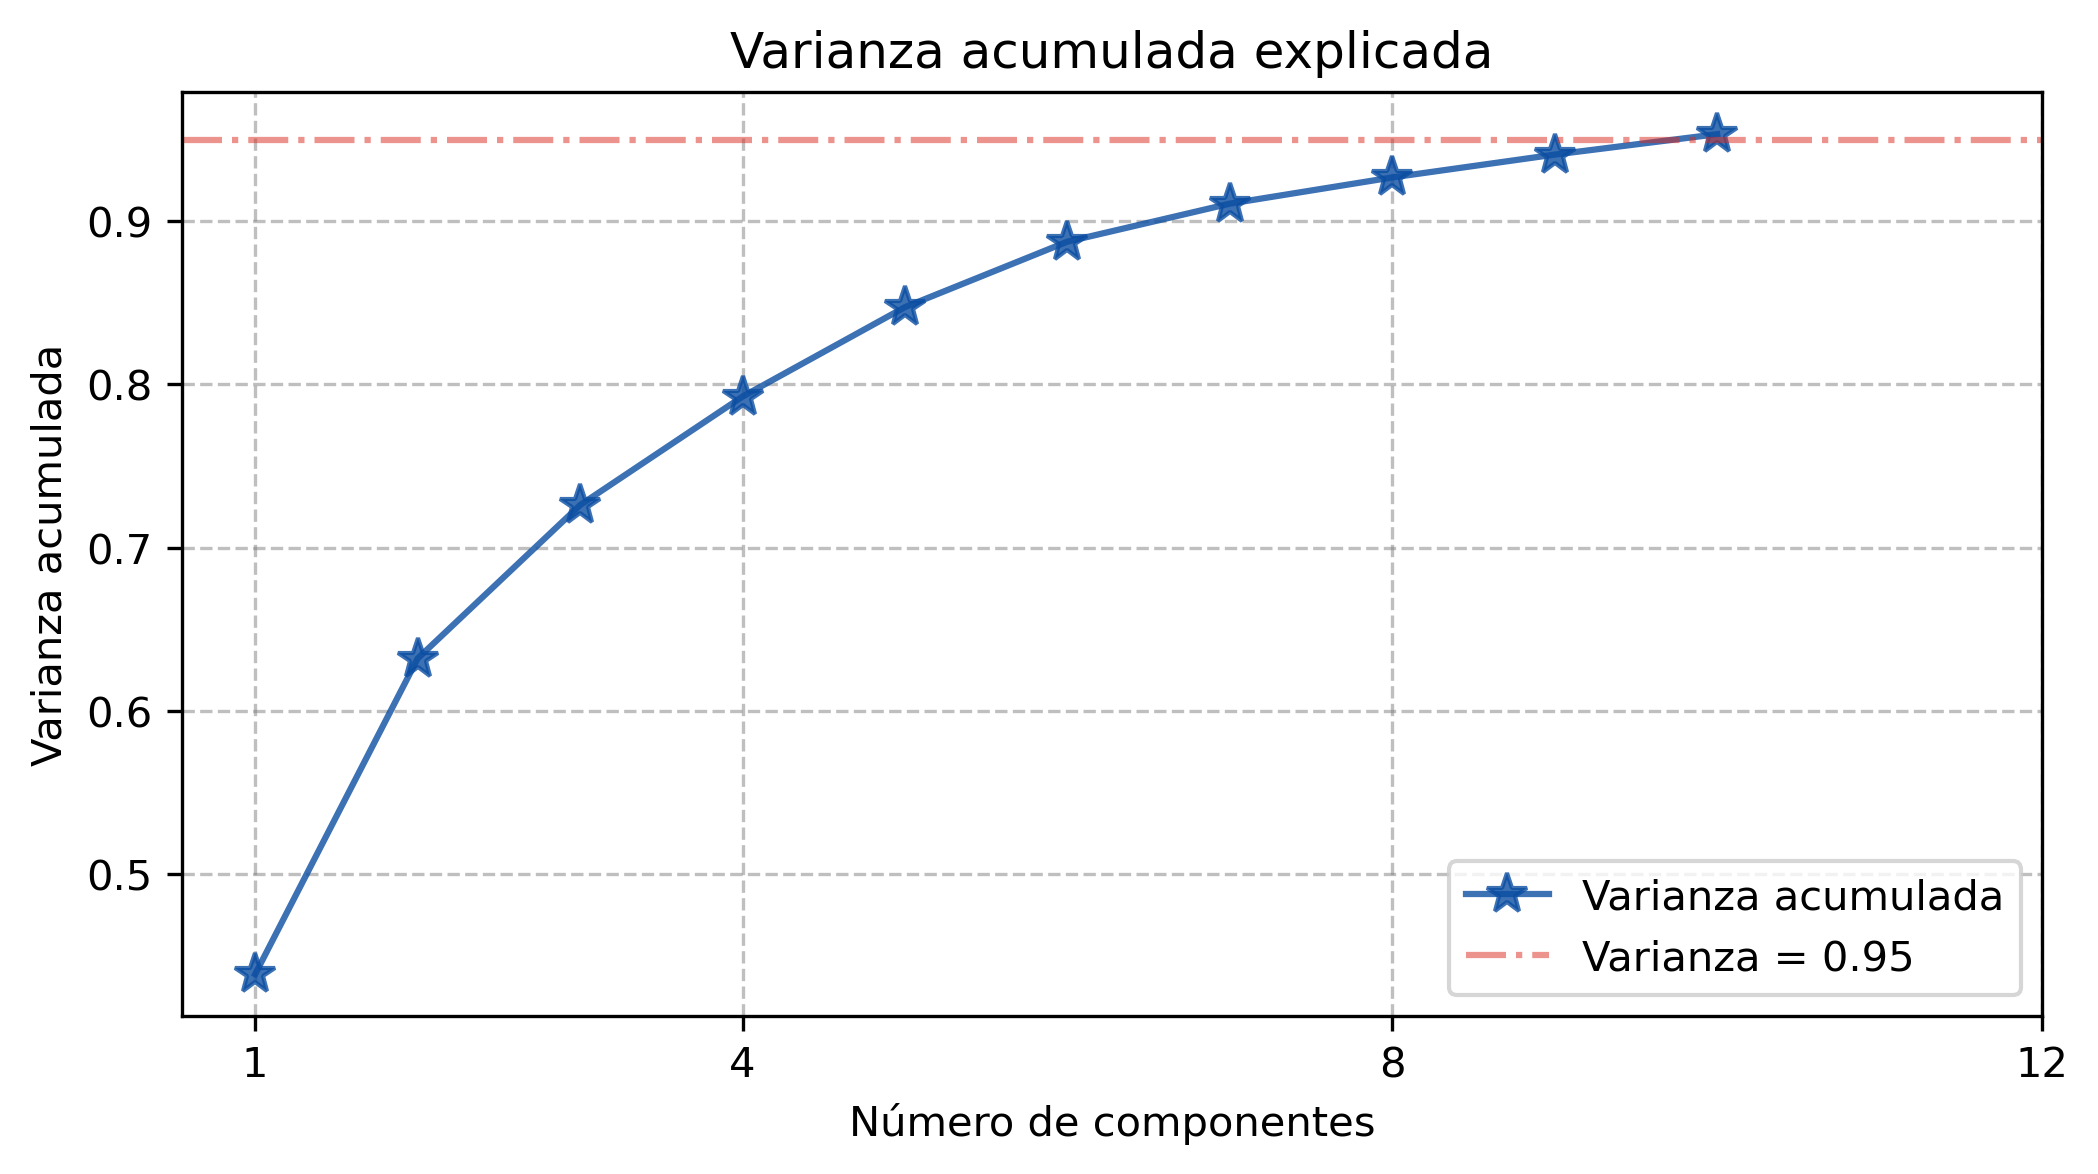
\includegraphics[width=0.85\textwidth]{Img/04_varianza_acumulada_pesea_var_95.png}
    \caption{Varianza acumulada al fijar PCA con $95\%$: bastan 10
        componentes para superar el umbral.}
    \label{fig:cancer-var-95}
\end{figure}

La proyección 2D (Figura~\ref{fig:cancer-pca-2d}) muestra que las clases
\textit{B} y \textit{M} son \textbf{linealmente separables casi por
    completo} ya en las dos primeras componentes principales. Este hecho
resulta clave para entender el alto desempeño que más adelante obtienen los
tres clasificadores: el problema es ``fácil'' geométricamente.

\begin{figure}[H]
    \centering
    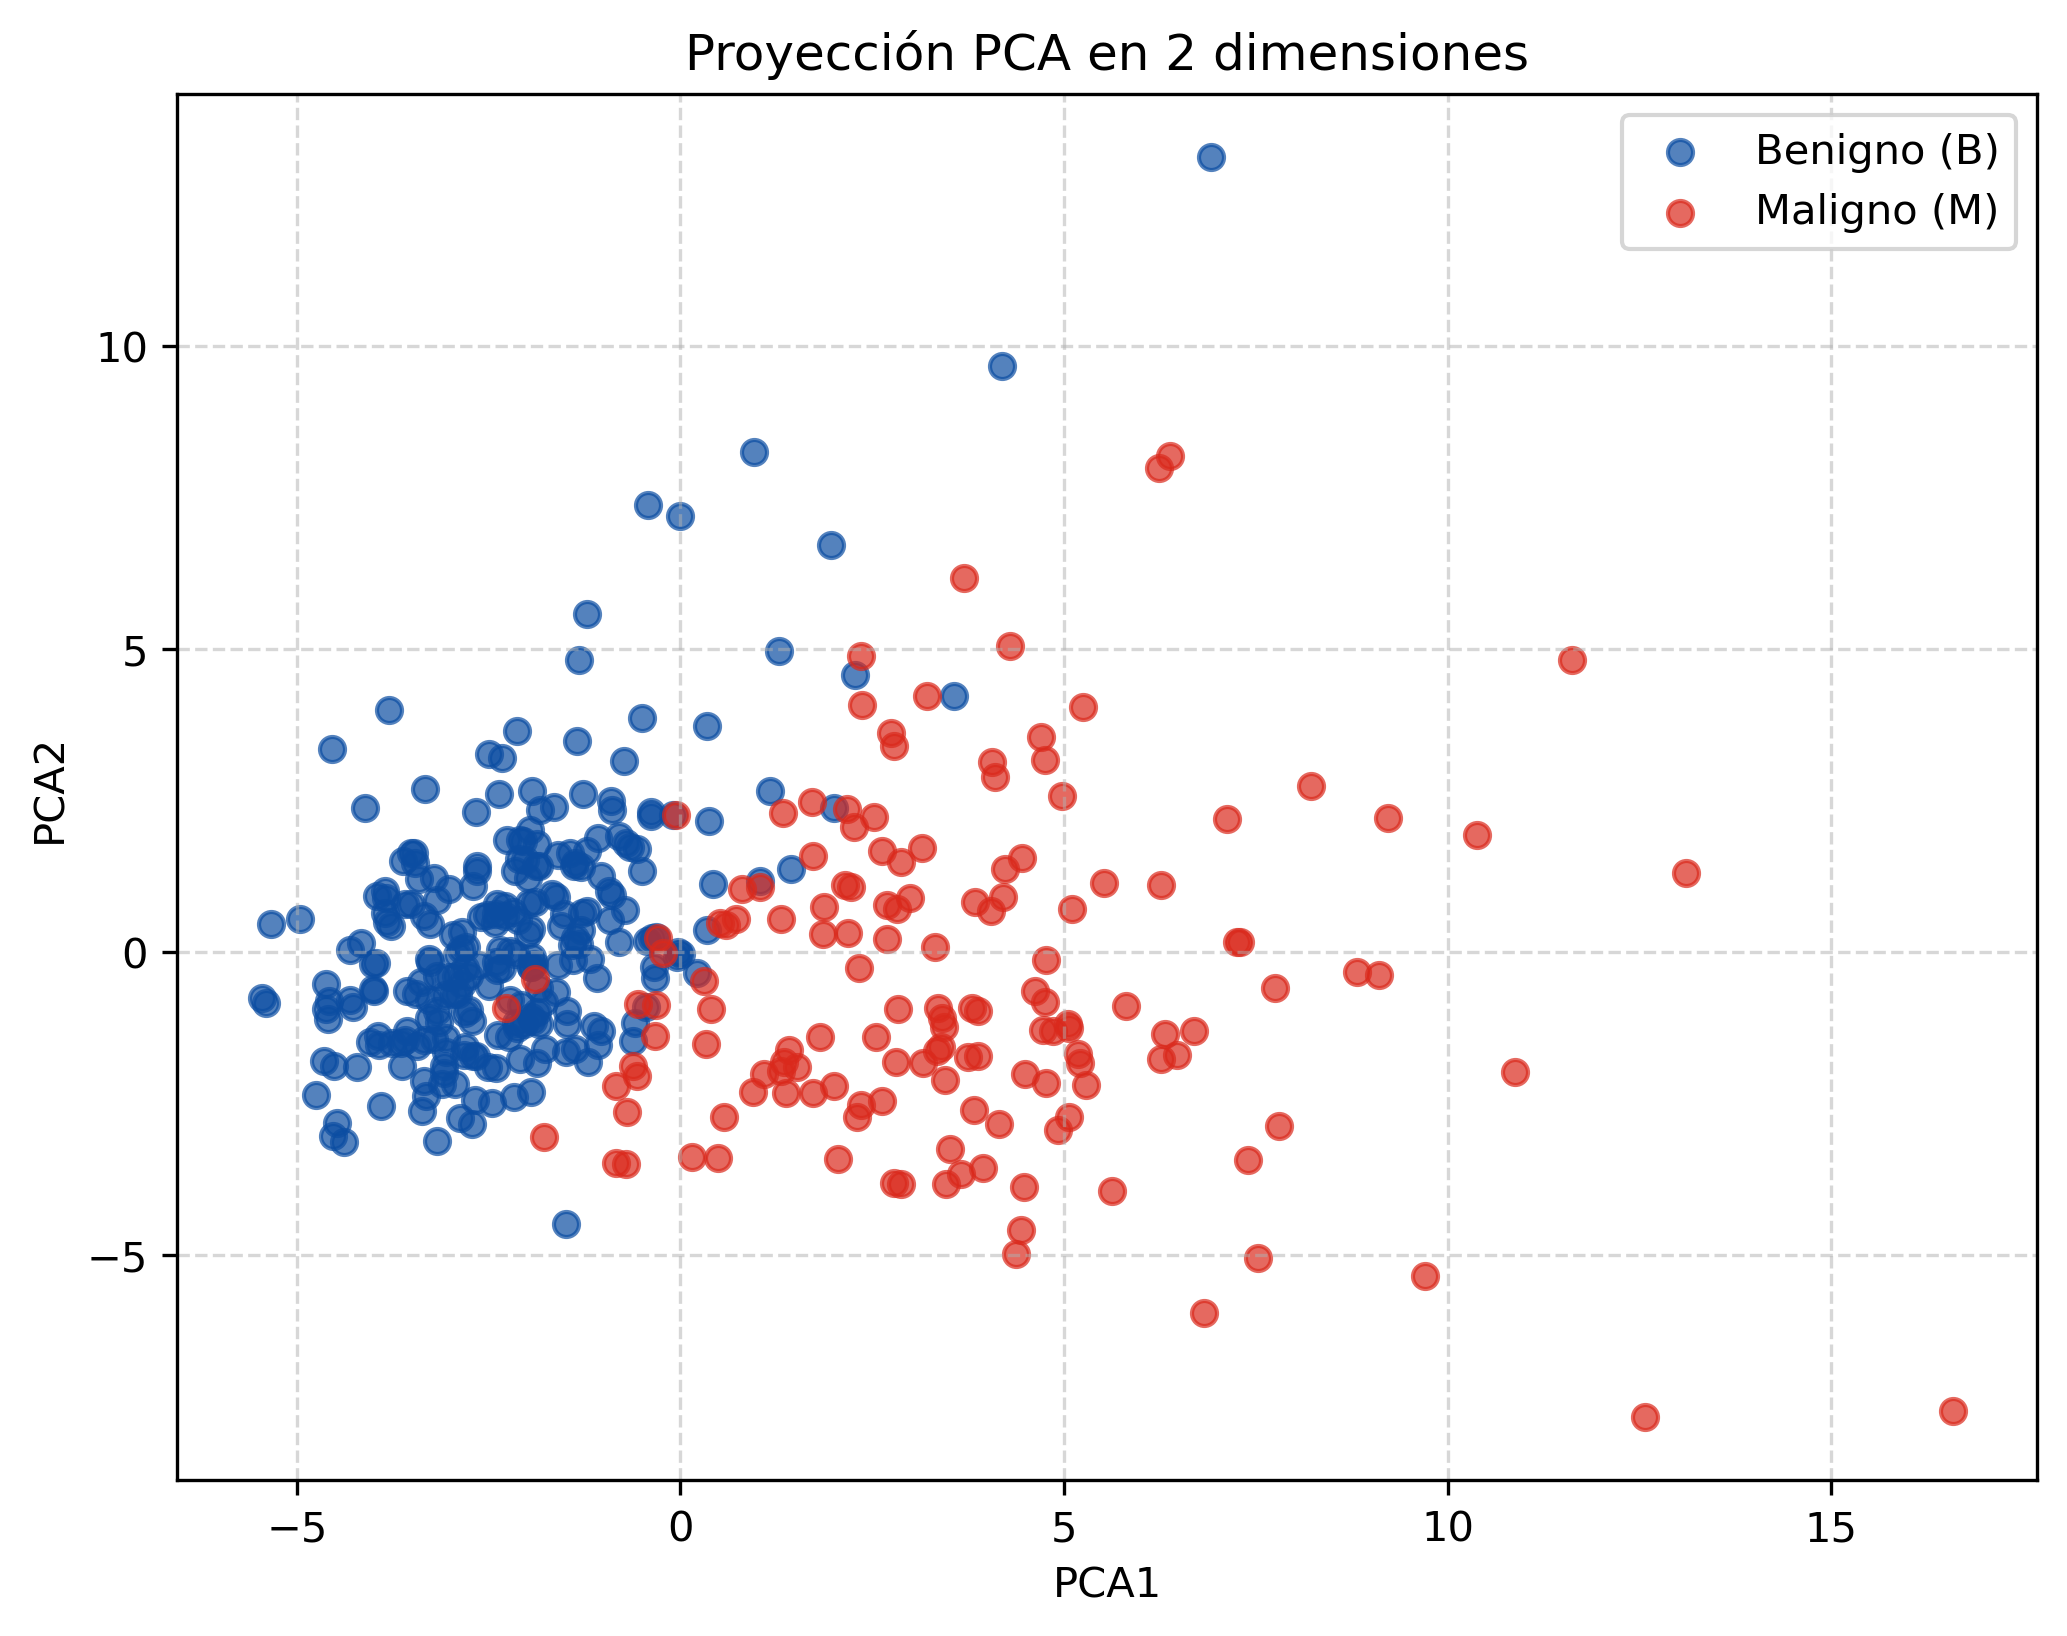
\includegraphics[width=0.80\textwidth]{Img/05_pca_2d.png}
    \caption{Proyección 2D de PCA sobre el conjunto de entrenamiento de
        Cancer. La separación entre clases es muy clara.}
    \label{fig:cancer-pca-2d}
\end{figure}

\subsubsection*{Pipelines, búsqueda en cuadrícula y resultados}

Se construyeron tres \texttt{Pipeline} con un único paso de clasificador
(KNN, árbol y SVM), todos entrenados sobre los datos balanceados con
SMOTE. La búsqueda en cuadrícula se realizó con \texttt{GridSearchCV}, CV
estratificada de 5 \textit{folds}, métrica \textit{accuracy} y
\texttt{n\_jobs = -1}. Los hiperparámetros explorados son los pedidos por
el enunciado (Sección~3.5). Los mejores resultados se resumen en la
Tabla~\ref{tab:cancer-resultados}.

\begin{table}[H]
    \centering
    \rowcolors{2}{rowgray}{white}
    \begin{tabular}{lccccc}
        \toprule
        \rowcolor{headerblue}
        \textcolor{headertext}{\textbf{Modelo}}                  &
        \textcolor{headertext}{\textbf{Mejores hiperparámetros}} &
        \textcolor{headertext}{\textbf{CV Acc.}}                 &
        \textcolor{headertext}{\textbf{Test Acc.}}               &
        \textcolor{headertext}{\textbf{Recall}}                  &
        \textcolor{headertext}{\textbf{F1}}                                                                                                                                            \\
        \midrule
        KNN                                                      & $k=9$, \textit{distance}, euclidean & $0.9860$          & $0.9532$          & $0.9688$          & $0.9394$          \\
        Árbol de Decisión                                        & gini, depth$=5$, split$=5$          & $0.9500$          & $0.9474$          & $0.9375$          & $0.9302$          \\
        SVM                                                      & lineal, $C=1$, $\gamma=$scale       & $\mathbf{0.9740}$ & $\mathbf{0.9766}$ & $\mathbf{0.9844}$ & $\mathbf{0.9692}$ \\
        \bottomrule
    \end{tabular}
    \caption{Resultados de los tres clasificadores sobre Cancer. El SVM
        lineal obtiene la mejor exactitud en prueba.}
    \label{tab:cancer-resultados}
\end{table}

La Figura~\ref{fig:cancer-confusion} muestra las matrices de confusión
sobre el conjunto de prueba. El SVM cae en apenas 4 errores de 171
muestras: 3 falsos positivos y 1 falso negativo. KNN comete 8 errores
(2 FP, 6 FN) y el árbol 9 (4 FP, 5 FN). En un contexto clínico real, el
\textit{recall} sobre la clase maligna (sensibilidad para no perder casos
positivos) es la métrica más relevante; bajo ese criterio el SVM también
domina con $0.9844$.

\begin{figure}[H]
    \centering
    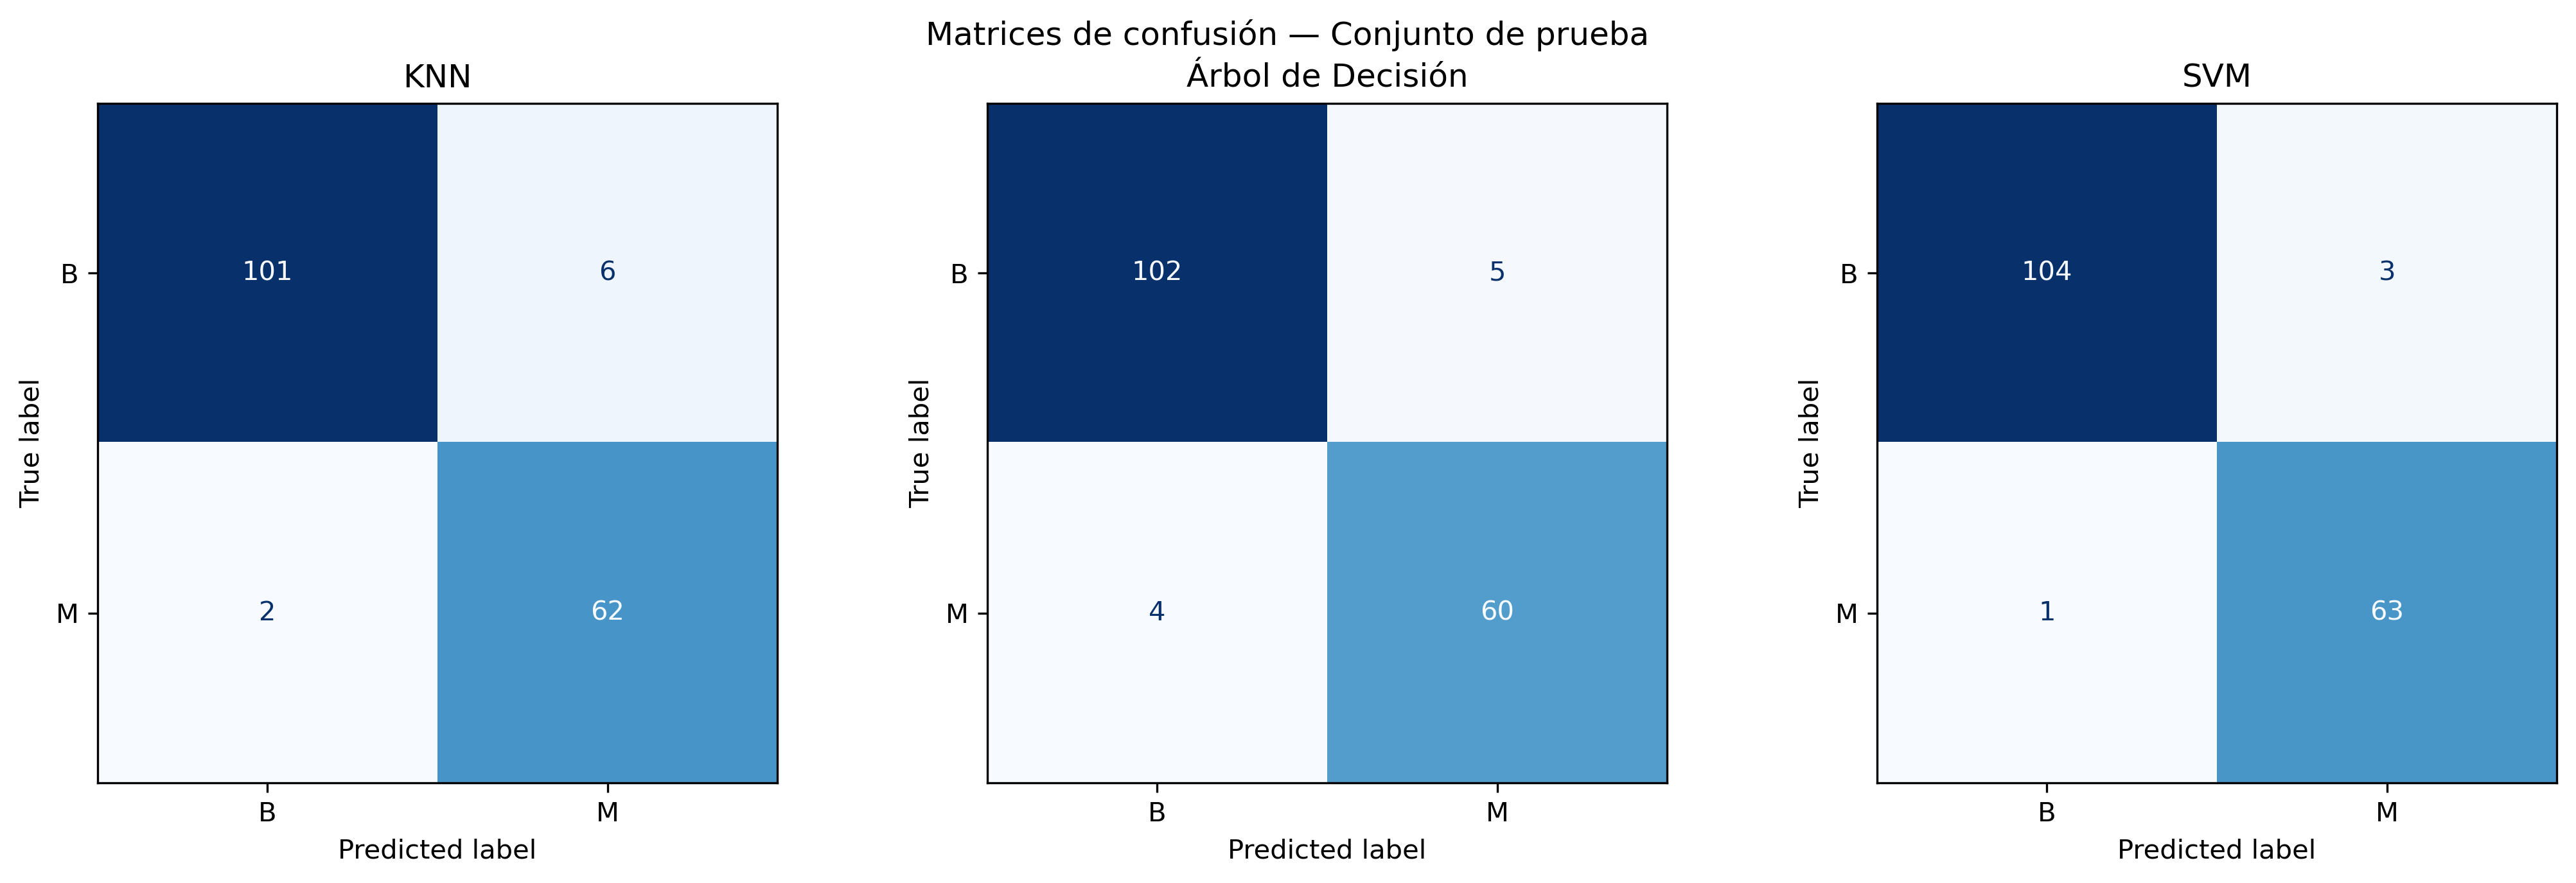
\includegraphics[width=1\textwidth]{Img/06_matrices_confusion_cancer.png}
    \caption{Matrices de confusión sobre el conjunto de prueba de Cancer
        para los tres modelos.}
    \label{fig:cancer-confusion}
\end{figure}

\subsubsection*{Fronteras de decisión en el espacio PCA 2D}

Para inspeccionar visualmente las fronteras, los tres clasificadores se
re-entrenaron sobre las dos primeras componentes principales calculadas
sobre el conjunto balanceado. Es importante señalar que estos modelos 2D
no son los que producen las métricas reportadas; sirven exclusivamente
como herramienta de visualización. La Figura~\ref{fig:cancer-fronteras}
muestra los tres modelos: el KNN produce una frontera \textit{fractal}
con regiones aisladas (esperable por su naturaleza local), el árbol
genera fronteras estrictamente ortogonales a los ejes (consecuencia
directa de las divisiones \textit{feature-by-feature}) y el SVM lineal
traza una recta limpia que separa las clases con un margen amplio.

\begin{figure}[H]
    \centering
    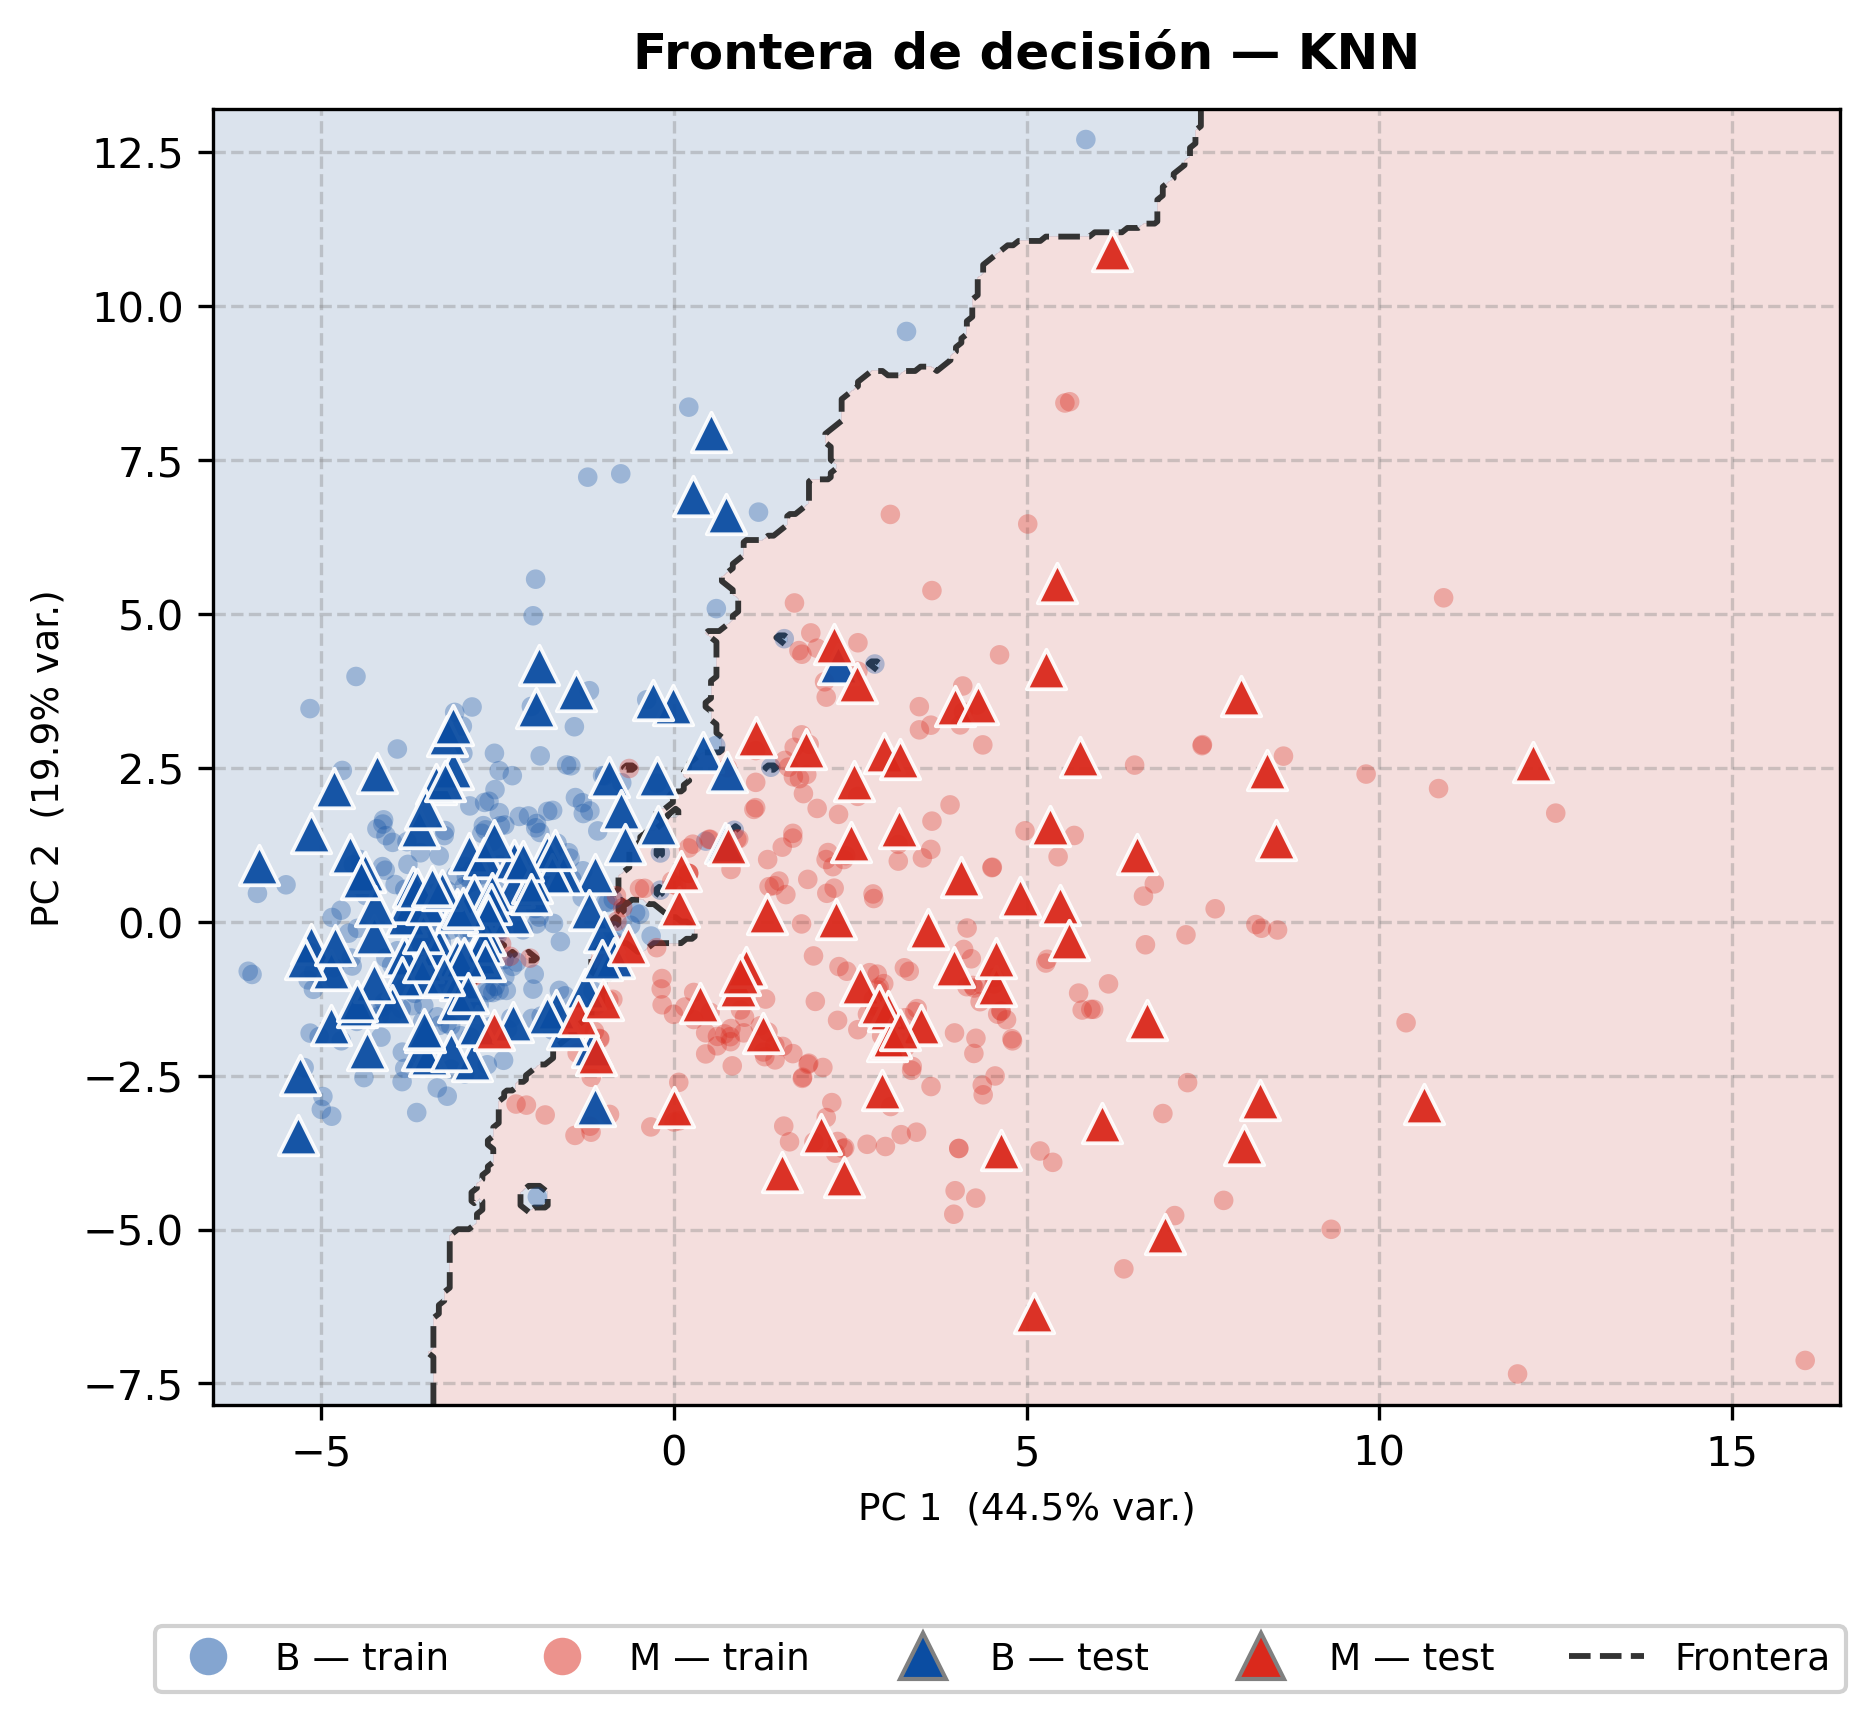
\includegraphics[width=0.49\textwidth]{Img/07a_frontera_knn.png}
    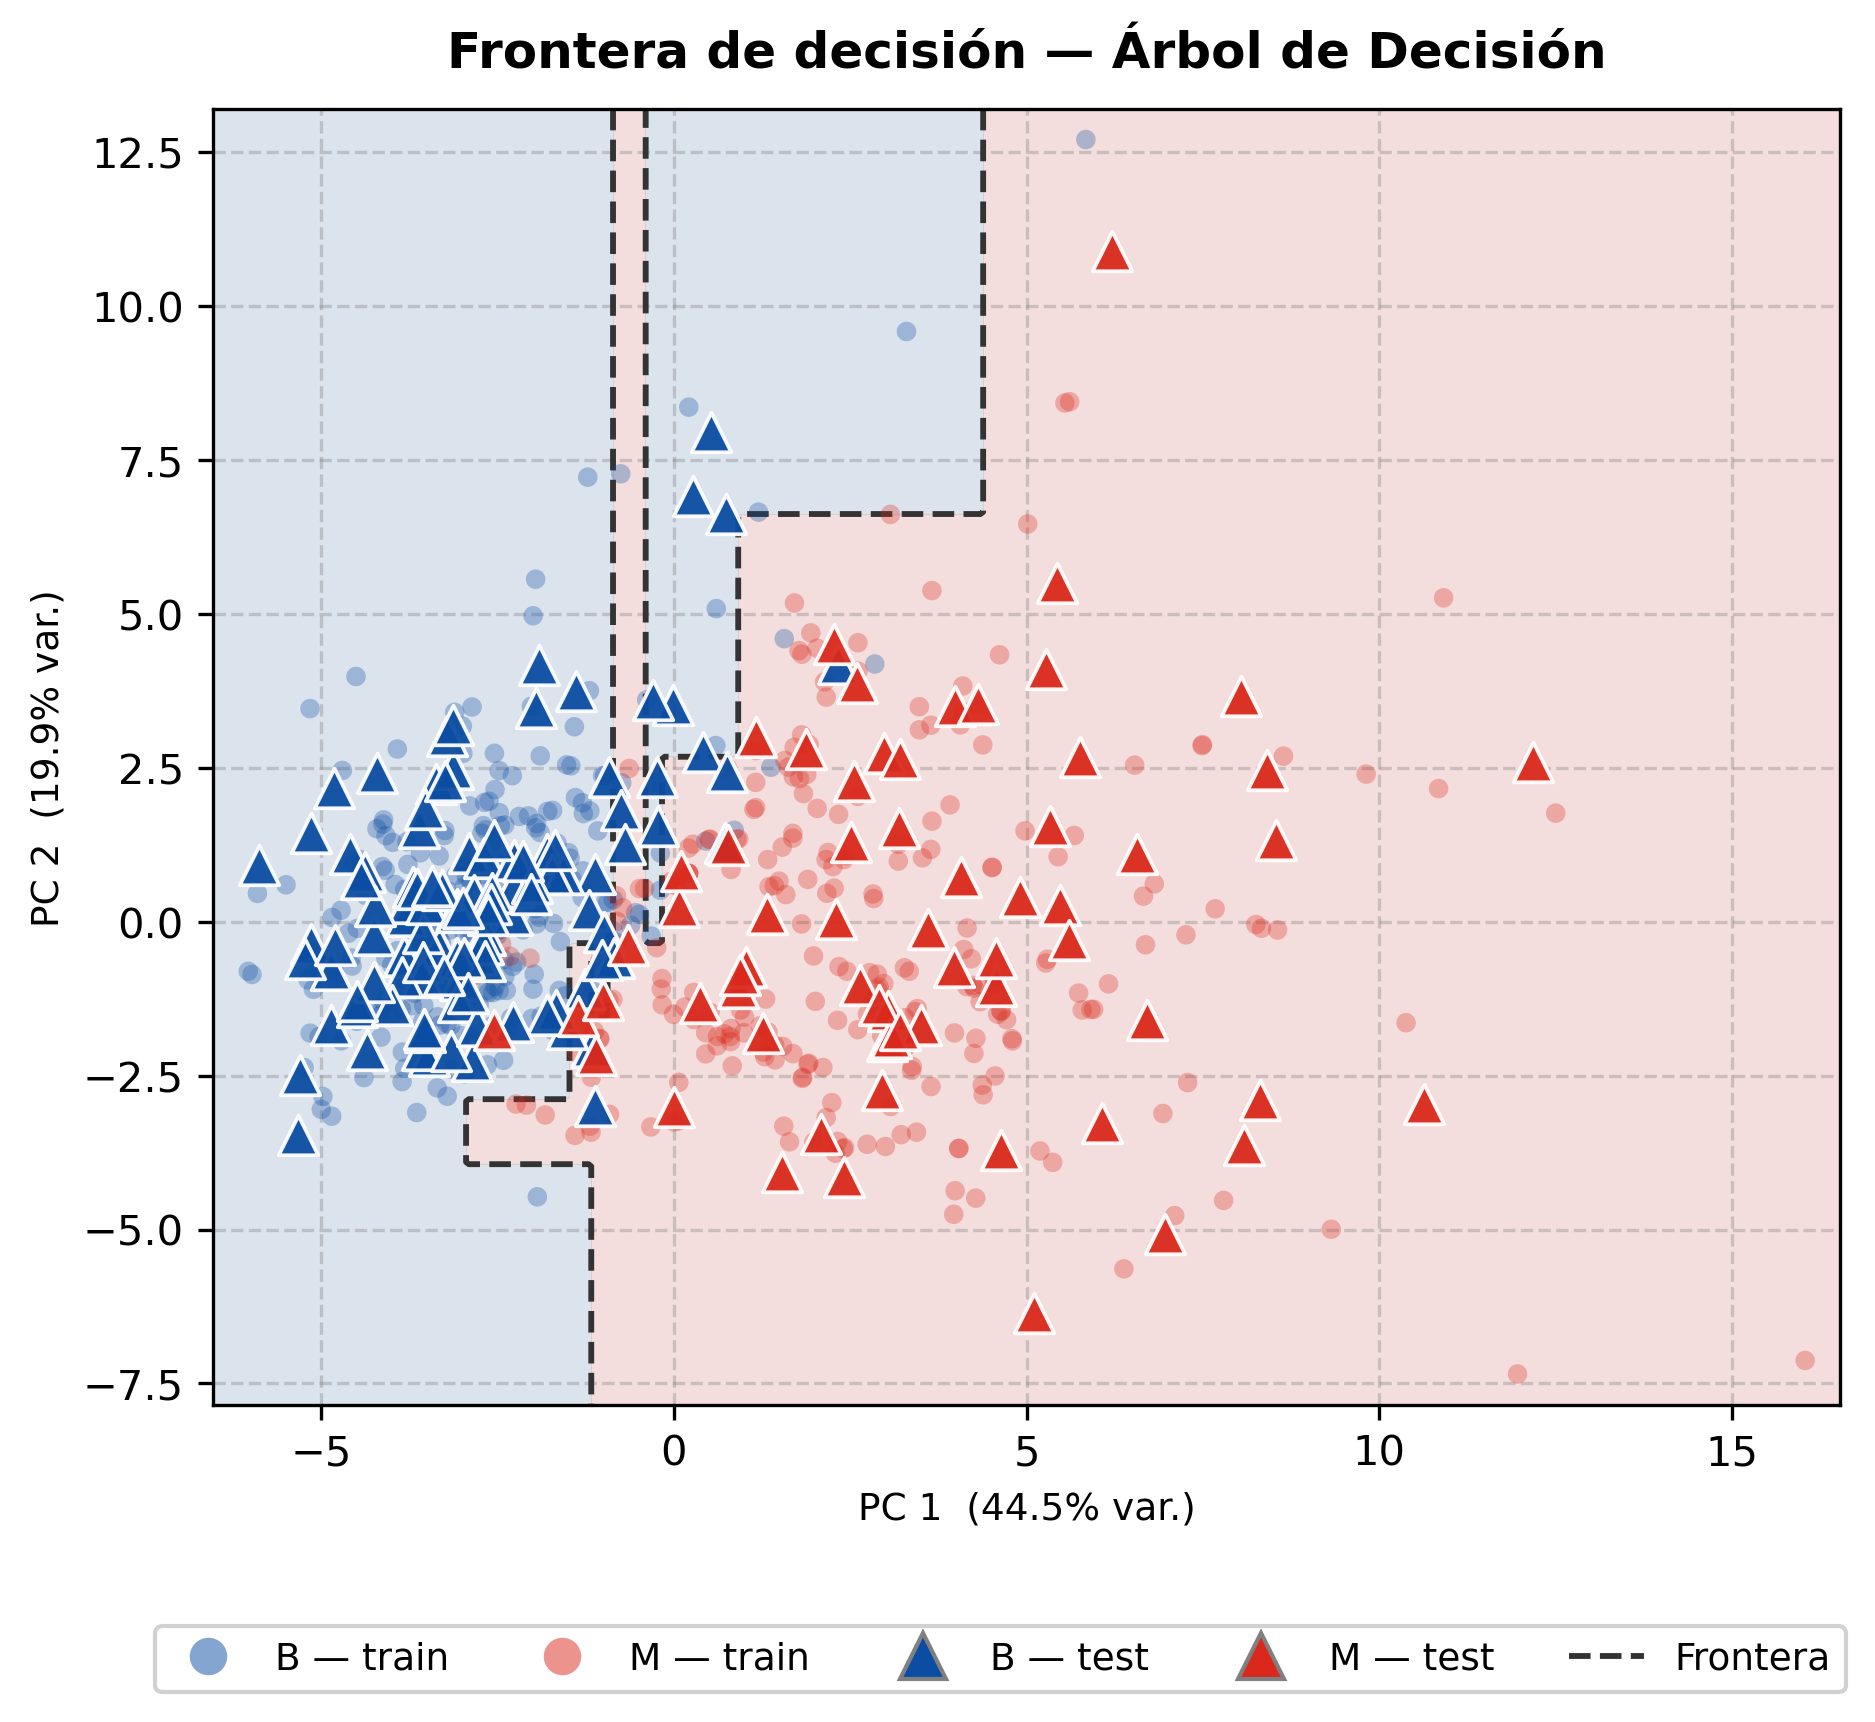
\includegraphics[width=0.49\textwidth]{Img/07b_frontera_arbol.png}
    \\[2mm]
    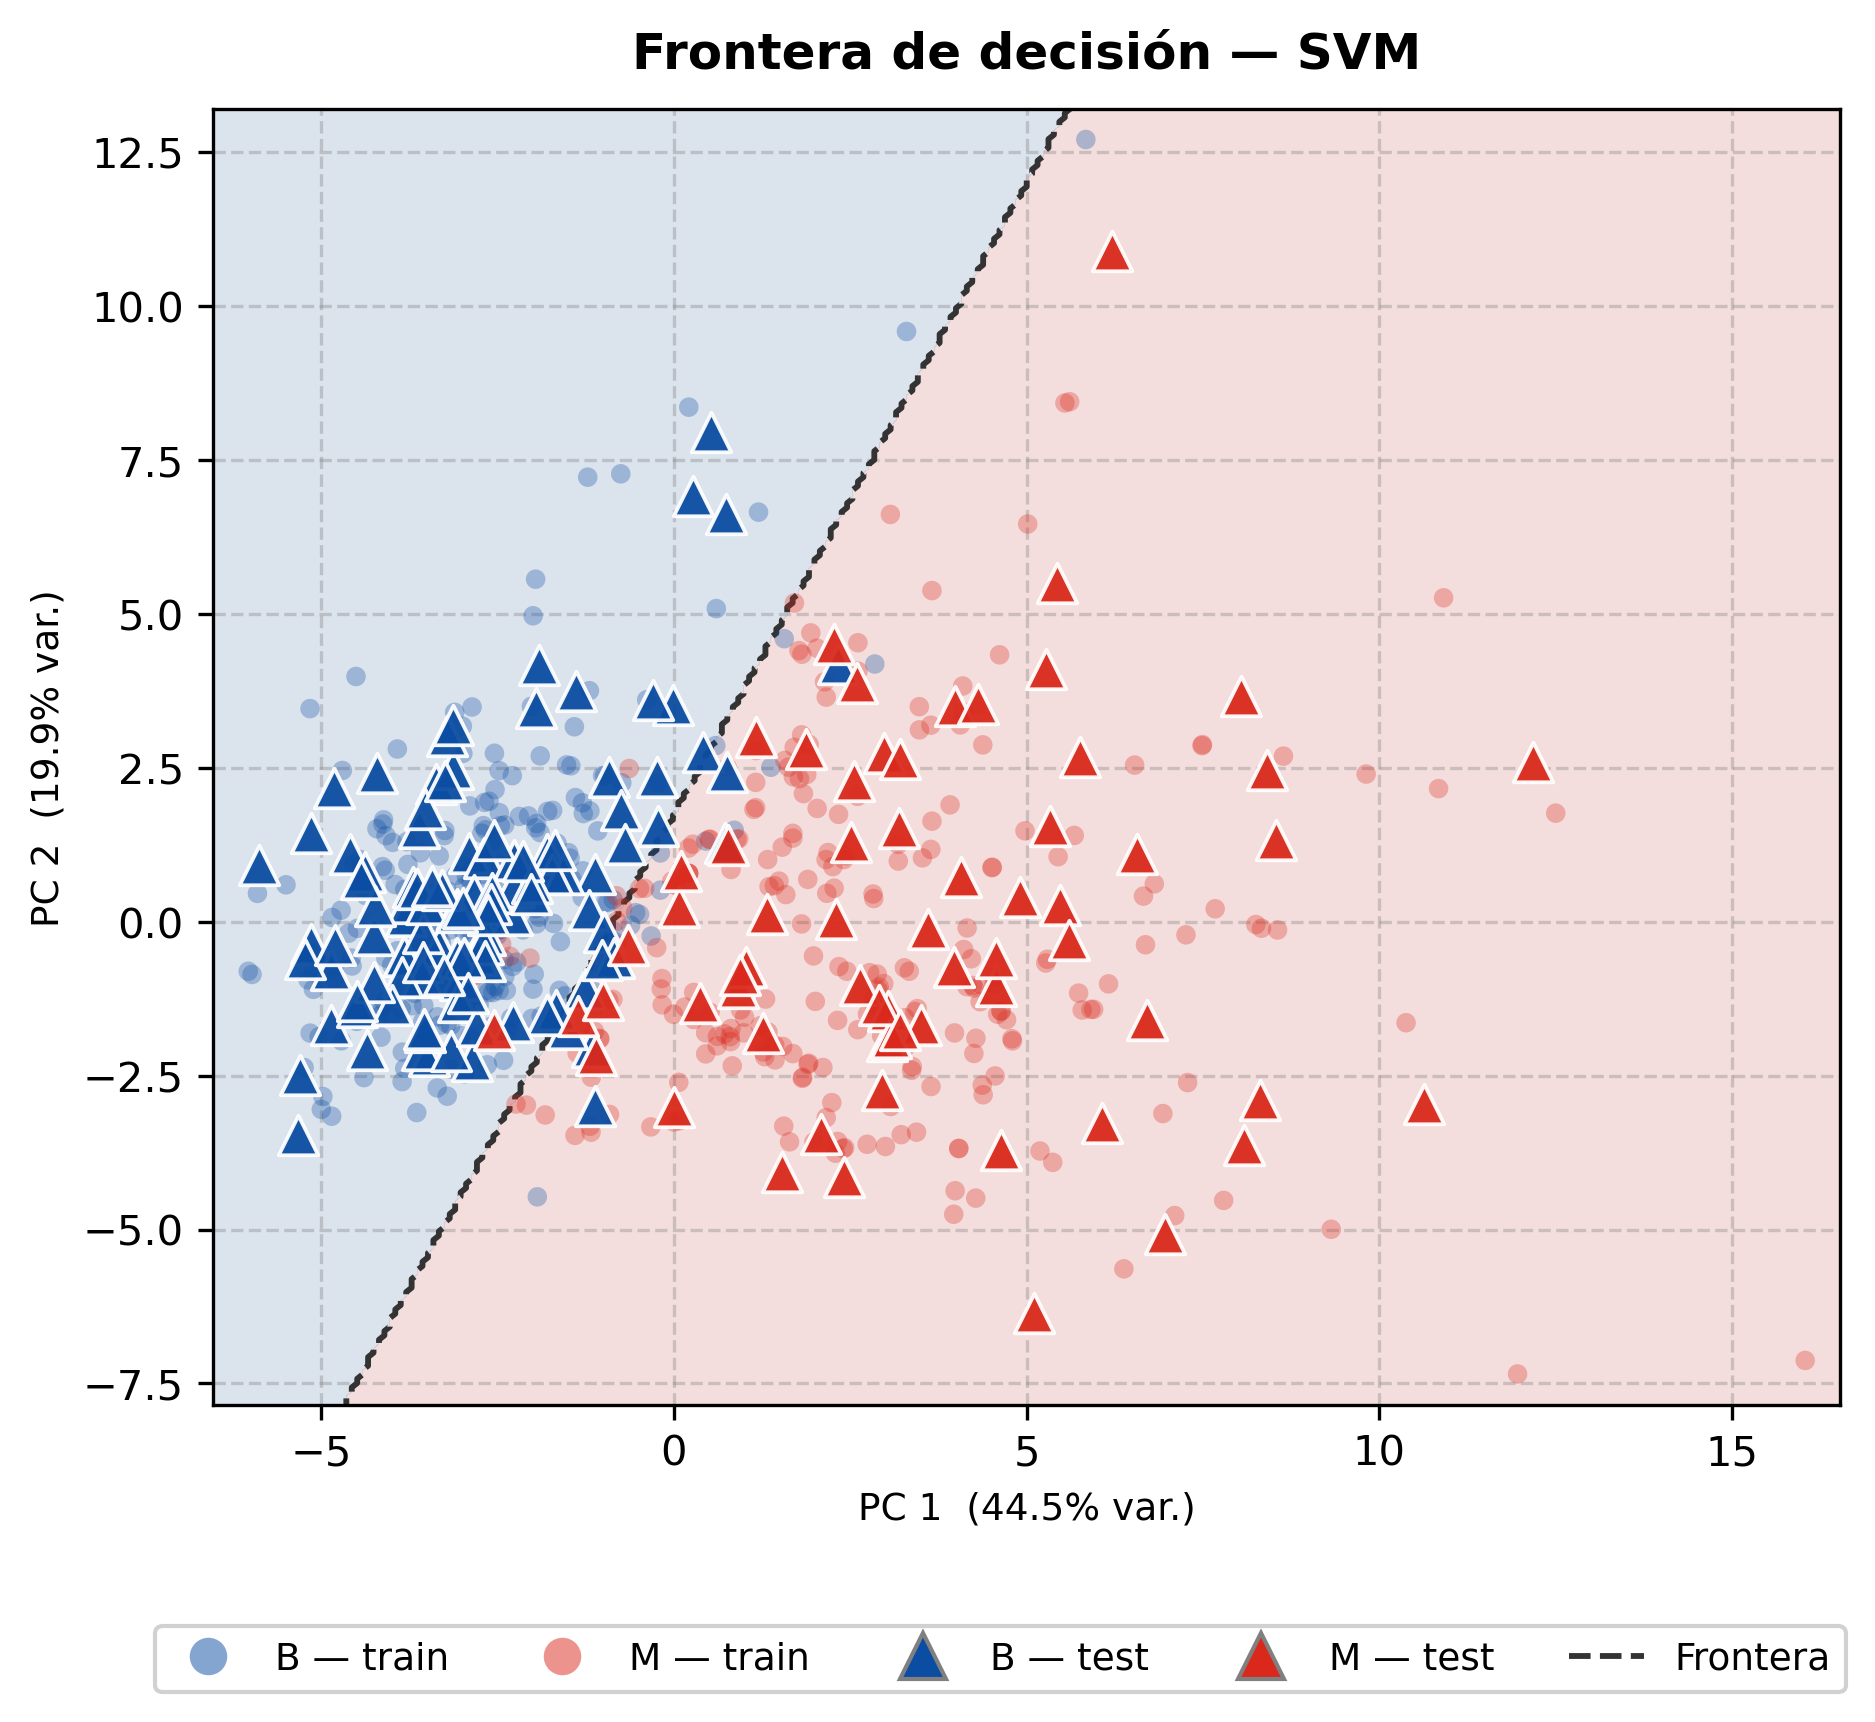
\includegraphics[width=0.49\textwidth]{Img/07c_frontera_svm.png}
    \caption{Fronteras de decisión en PCA 2D para Cancer: KNN (arriba
        izquierda), árbol (arriba derecha) y SVM lineal (abajo).}
    \label{fig:cancer-fronteras}
\end{figure}

\subsubsection*{Árbol de decisión}

La Figura~\ref{fig:cancer-arbol} presenta el árbol entrenado con los
mejores hiperparámetros (gini, profundidad $5$, división mínima $5$). El
nodo raíz divide por \texttt{concave\_points\_worst}, una de las
características que el perfilamiento ya señalaba como fuertemente
discriminativa. Subsiguientes divisiones usan \texttt{texture\_worst},
\texttt{radius\_worst} y \texttt{area\_se}, lo que es coherente con el
hecho biomédico de que los tumores malignos tienden a tener bordes más
irregulares y mayor tamaño.

\begin{figure}[H]
    \centering
    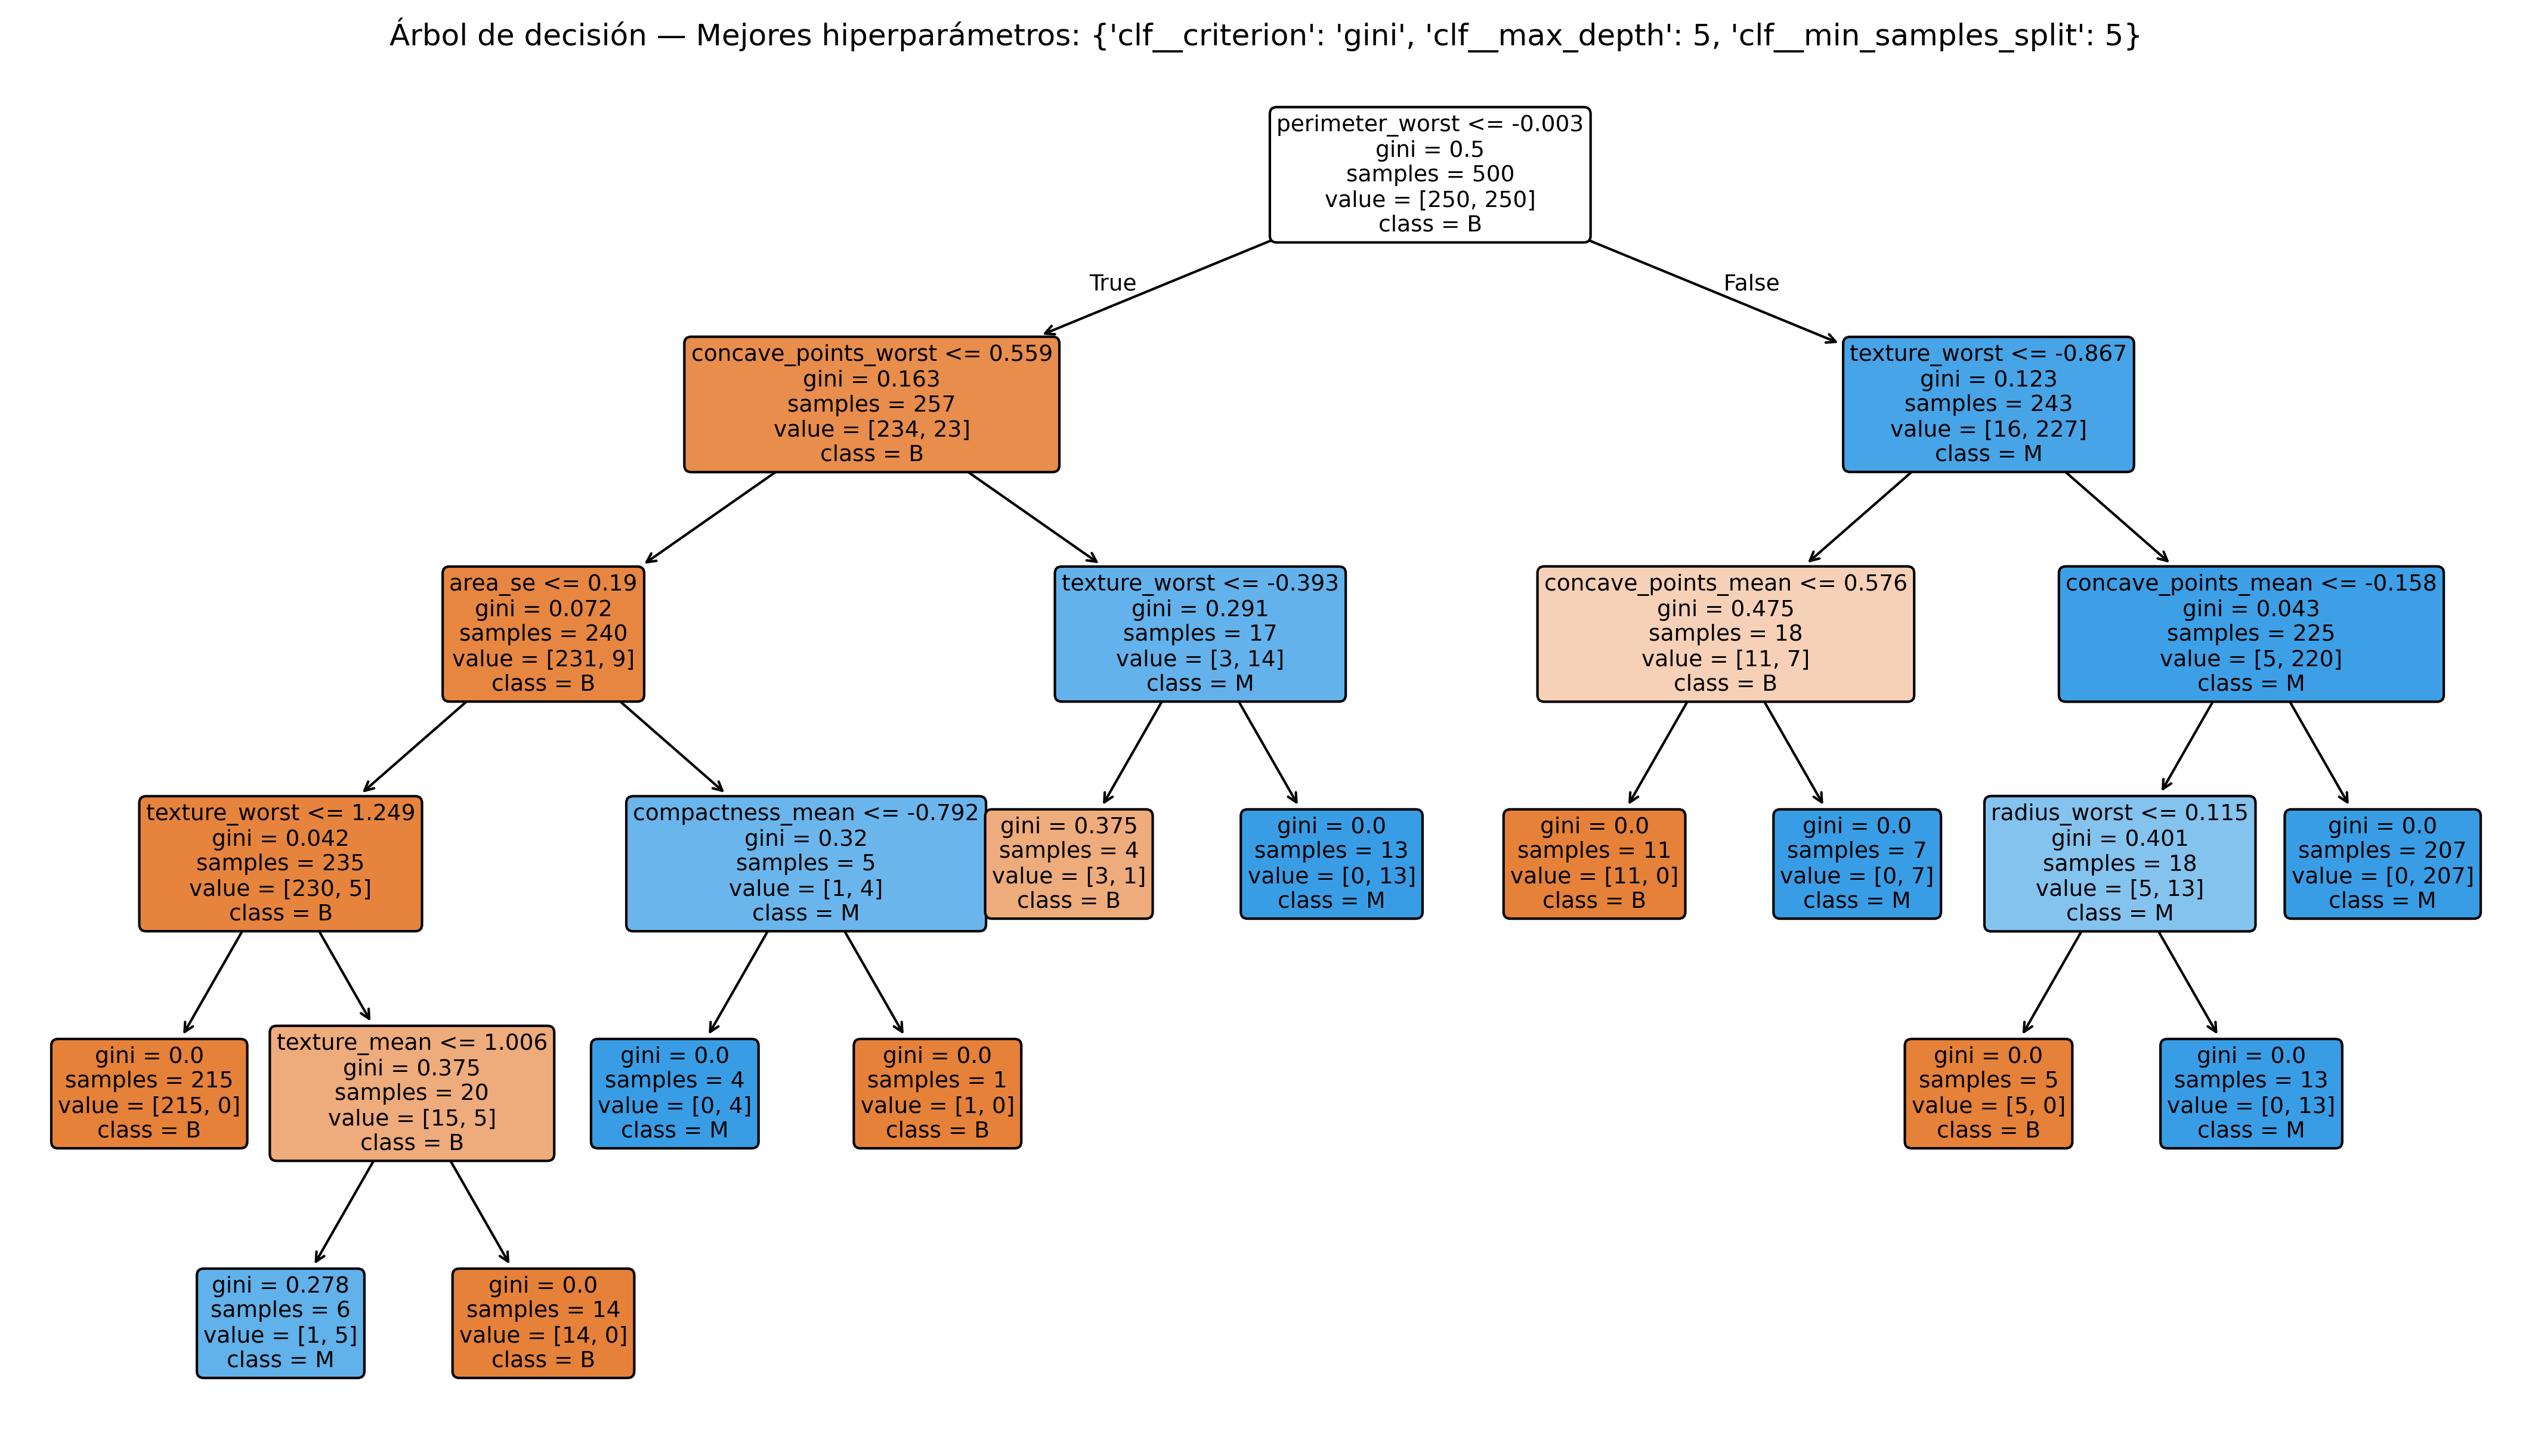
\includegraphics[width=1\textwidth]{Img/08_arbol_decision_cancer.png}
    \caption{Árbol de decisión entrenado sobre Cancer con los mejores
        hiperparámetros.}
    \label{fig:cancer-arbol}
\end{figure}

\subsubsection*{Comparación e hiperparámetro más relevante}

La Figura~\ref{fig:cancer-comparacion} contrasta exactitud en CV vs
exactitud en prueba. Llama la atención que KNN, que en CV obtuvo el
mejor resultado ($0.9860$), cae en prueba a $0.9532$: es la mayor
\textit{brecha} entre los tres modelos. Esto sugiere un cierto
sobreajuste del KNN al conjunto balanceado por SMOTE (los puntos
sintéticos son interpolaciones que el algoritmo de vecinos memoriza
sin esfuerzo). El SVM, en cambio, generaliza mejor: pasa de $0.9740$ en
CV a $0.9766$ en prueba ---una ligera mejora atribuible a la varianza
muestral---.

\begin{figure}[H]
    \centering
    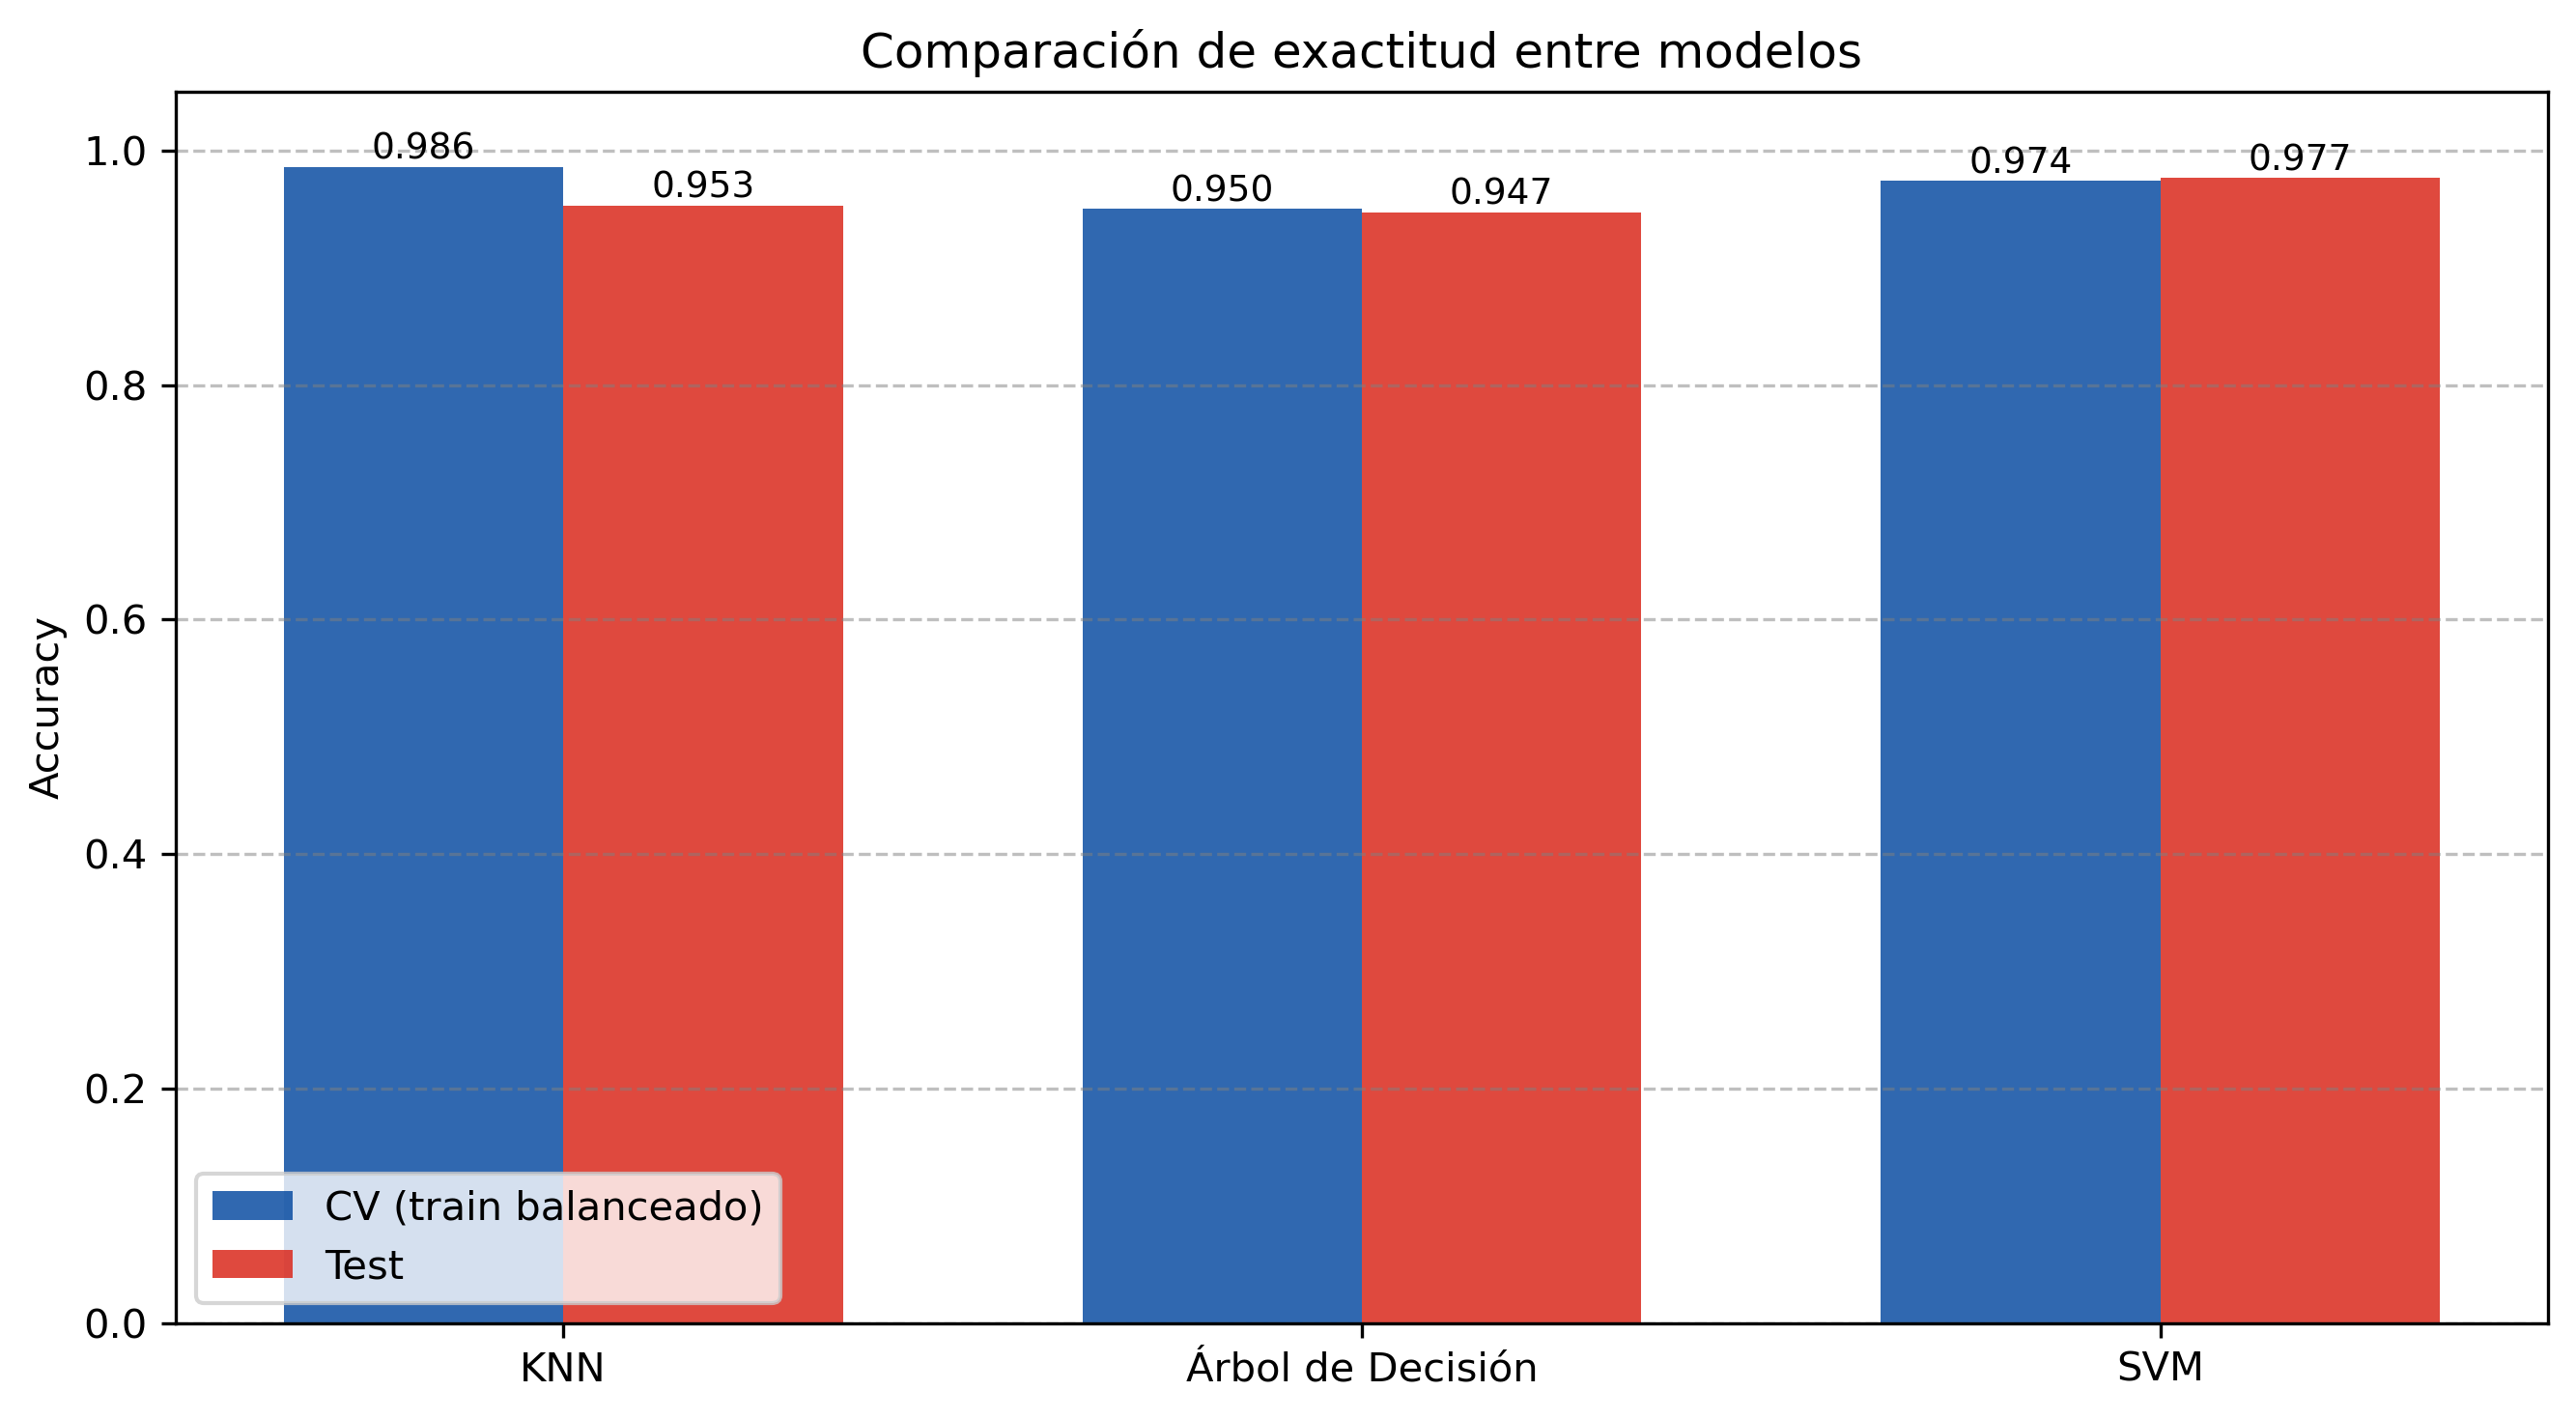
\includegraphics[width=0.85\textwidth]{Img/09_comparacion_exactitud_cancer.png}
    \caption{Comparación de exactitud CV vs Test para los tres modelos
        sobre Cancer.}
    \label{fig:cancer-comparacion}
\end{figure}

Para identificar el hiperparámetro más relevante de cada modelo se calculó,
sobre los resultados del \texttt{cv\_results\_}, el rango (máximo menos
mínimo) del \textit{accuracy} promedio al fijar cada hiperparámetro en
sus posibles valores. Los resultados se muestran en la
Tabla~\ref{tab:cancer-hiperparametros}.

\begin{table}[H]
    \centering
    \rowcolors{2}{rowgray}{white}
    \begin{tabular}{lll}
        \toprule
        \rowcolor{headerblue}
        \textcolor{headertext}{\textbf{Modelo}}                       &
        \textcolor{headertext}{\textbf{Hiperparámetro más relevante}} &
        \textcolor{headertext}{\textbf{$\Delta$ accuracy}}                                            \\
        \midrule
        KNN                                                           & \texttt{weights}   & $0.0110$ \\
        Árbol de Decisión                                             & \texttt{criterion} & $0.0112$ \\
        SVM                                                           & \texttt{C}         & $0.0152$ \\
        \bottomrule
    \end{tabular}
    \caption{Hiperparámetro más sensible por modelo sobre Cancer.}
    \label{tab:cancer-hiperparametros}
\end{table}

Las diferencias absolutas son pequeñas (de orden $10^{-2}$) porque el
problema es tan separable que todos los modelos alcanzan ya valores muy
altos. Aun así, los resultados son coherentes con la teoría: en KNN el
peso de los vecinos importa más que el número exacto cuando $k$ es
moderado; en árboles el criterio \textit{gini}/\textit{entropy} fija el
sesgo inductivo del crecimiento; y en SVM la regularización $C$ controla
directamente la tolerancia a errores y por tanto la geometría del
margen.

\subsection{Conjunto de datos: Heart Disease}

\subsubsection*{Carga, combinación de fuentes y reformulación binaria}

El conjunto \textbf{Heart Disease} del UCI Machine Learning Repository
está dividido en cuatro archivos correspondientes a los hospitales que
recolectaron los datos: \texttt{cleveland} (303 instancias),
\texttt{hungarian} (294), \texttt{switzerland} (123) y \texttt{va} (200).
Para esta práctica se concatenaron los cuatro en un único
\texttt{DataFrame} de \textbf{920 instancias} y 14 columnas, añadiendo
una variable auxiliar \texttt{origen} para mantener la trazabilidad. La
variable objetivo original \texttt{num} toma valores enteros entre $0$ y
$4$ (donde $0$ es ausencia de enfermedad y $1\!-\!4$ distintos grados de
afectación). Por consistencia con la literatura clásica del conjunto y
para simplificar el problema a una clasificación binaria, se reformuló
como \texttt{target = num > 0}, obteniendo 411 sanos y 509 enfermos. El
desbalance es leve (\textit{ratio} $1.24$).

\subsubsection*{Análisis de valores faltantes: el reto principal}

A diferencia del conjunto Cancer, Heart Disease presenta una proporción
muy alta de valores faltantes, fuertemente concentrada por archivo de
origen. La Tabla~\ref{tab:heart-faltantes} desglosa los porcentajes
globales y por hospital.

\begin{table}[H]
    \centering
    \rowcolors{2}{rowgray}{white}
    \begin{tabular}{lcccc}
        \toprule
        \rowcolor{headerblue}
        \textcolor{headertext}{\textbf{Variable}}         &
        \textcolor{headertext}{\textbf{Global (\%)}}      &
        \textcolor{headertext}{\textbf{Hungarian (\%)}}   &
        \textcolor{headertext}{\textbf{Switzerland (\%)}} &
        \textcolor{headertext}{\textbf{VA (\%)}}                                              \\
        \midrule
        \texttt{ca}                                       & $66.4$ & $99.0$ & $95.9$ & $99.0$ \\
        \texttt{thal}                                     & $52.8$ & $90.5$ & $42.3$ & $83.0$ \\
        \texttt{slope}                                    & $33.6$ & $64.6$ & $13.8$ & $51.0$ \\
        \texttt{fbs}                                      & $9.8$  & $2.7$  & $61.0$ & $3.5$  \\
        \texttt{oldpeak}                                  & $6.7$  & $0.0$  & $4.9$  & $28.0$ \\
        \texttt{trestbps}                                 & $6.4$  & $0.3$  & $1.6$  & $28.0$ \\
        \texttt{thalach}                                  & $6.0$  & $0.3$  & $0.8$  & $26.5$ \\
        \texttt{exang}                                    & $6.0$  & $0.3$  & $0.8$  & $26.5$ \\
        \texttt{chol}                                     & $3.3$  & $7.8$  & $0.0$  & $3.5$  \\
        \bottomrule
    \end{tabular}
    \caption{Distribución de valores faltantes en Heart Disease, global y
        por archivo de origen.}
    \label{tab:heart-faltantes}
\end{table}

El patrón es revelador: \texttt{ca}, \texttt{thal} y \texttt{slope} están
prácticamente ausentes fuera de Cleveland, lo que sugiere que esos
hospitales simplemente no registraron esas pruebas. Dado que descartarlas
completas sería renunciar a información valiosa para los casos donde
sí están disponibles, se optó por \textbf{imputar}: mediana para las
variables continuas (\texttt{age}, \texttt{trestbps}, \texttt{chol},
\texttt{thalach}, \texttt{oldpeak}, \texttt{ca}) y moda
(\textit{most\_frequent}) para las codificadas categóricamente
(\texttt{sex}, \texttt{cp}, \texttt{fbs}, \texttt{restecg},
\texttt{exang}, \texttt{slope}, \texttt{thal}). Esta decisión introduce un
sesgo controlado ---la mediana/moda no preserva la varianza condicional
de las relaciones entre variables--- pero es defendible dada la escala
del problema.

\subsubsection*{Variables continuas vs categóricas codificadas}

Heart Disease contiene 13 predictoras, de las cuales 6 son continuas y 7
son categóricas codificadas como números (binarias u ordinales). La
Figura~\ref{fig:heart-distribucion} muestra la distribución del objetivo
binario y la Figura~\ref{fig:heart-boxplots} compara las distribuciones
de las variables continuas para los grupos \textit{Sano} vs
\textit{Enfermo}.

\begin{figure}[H]
    \centering
    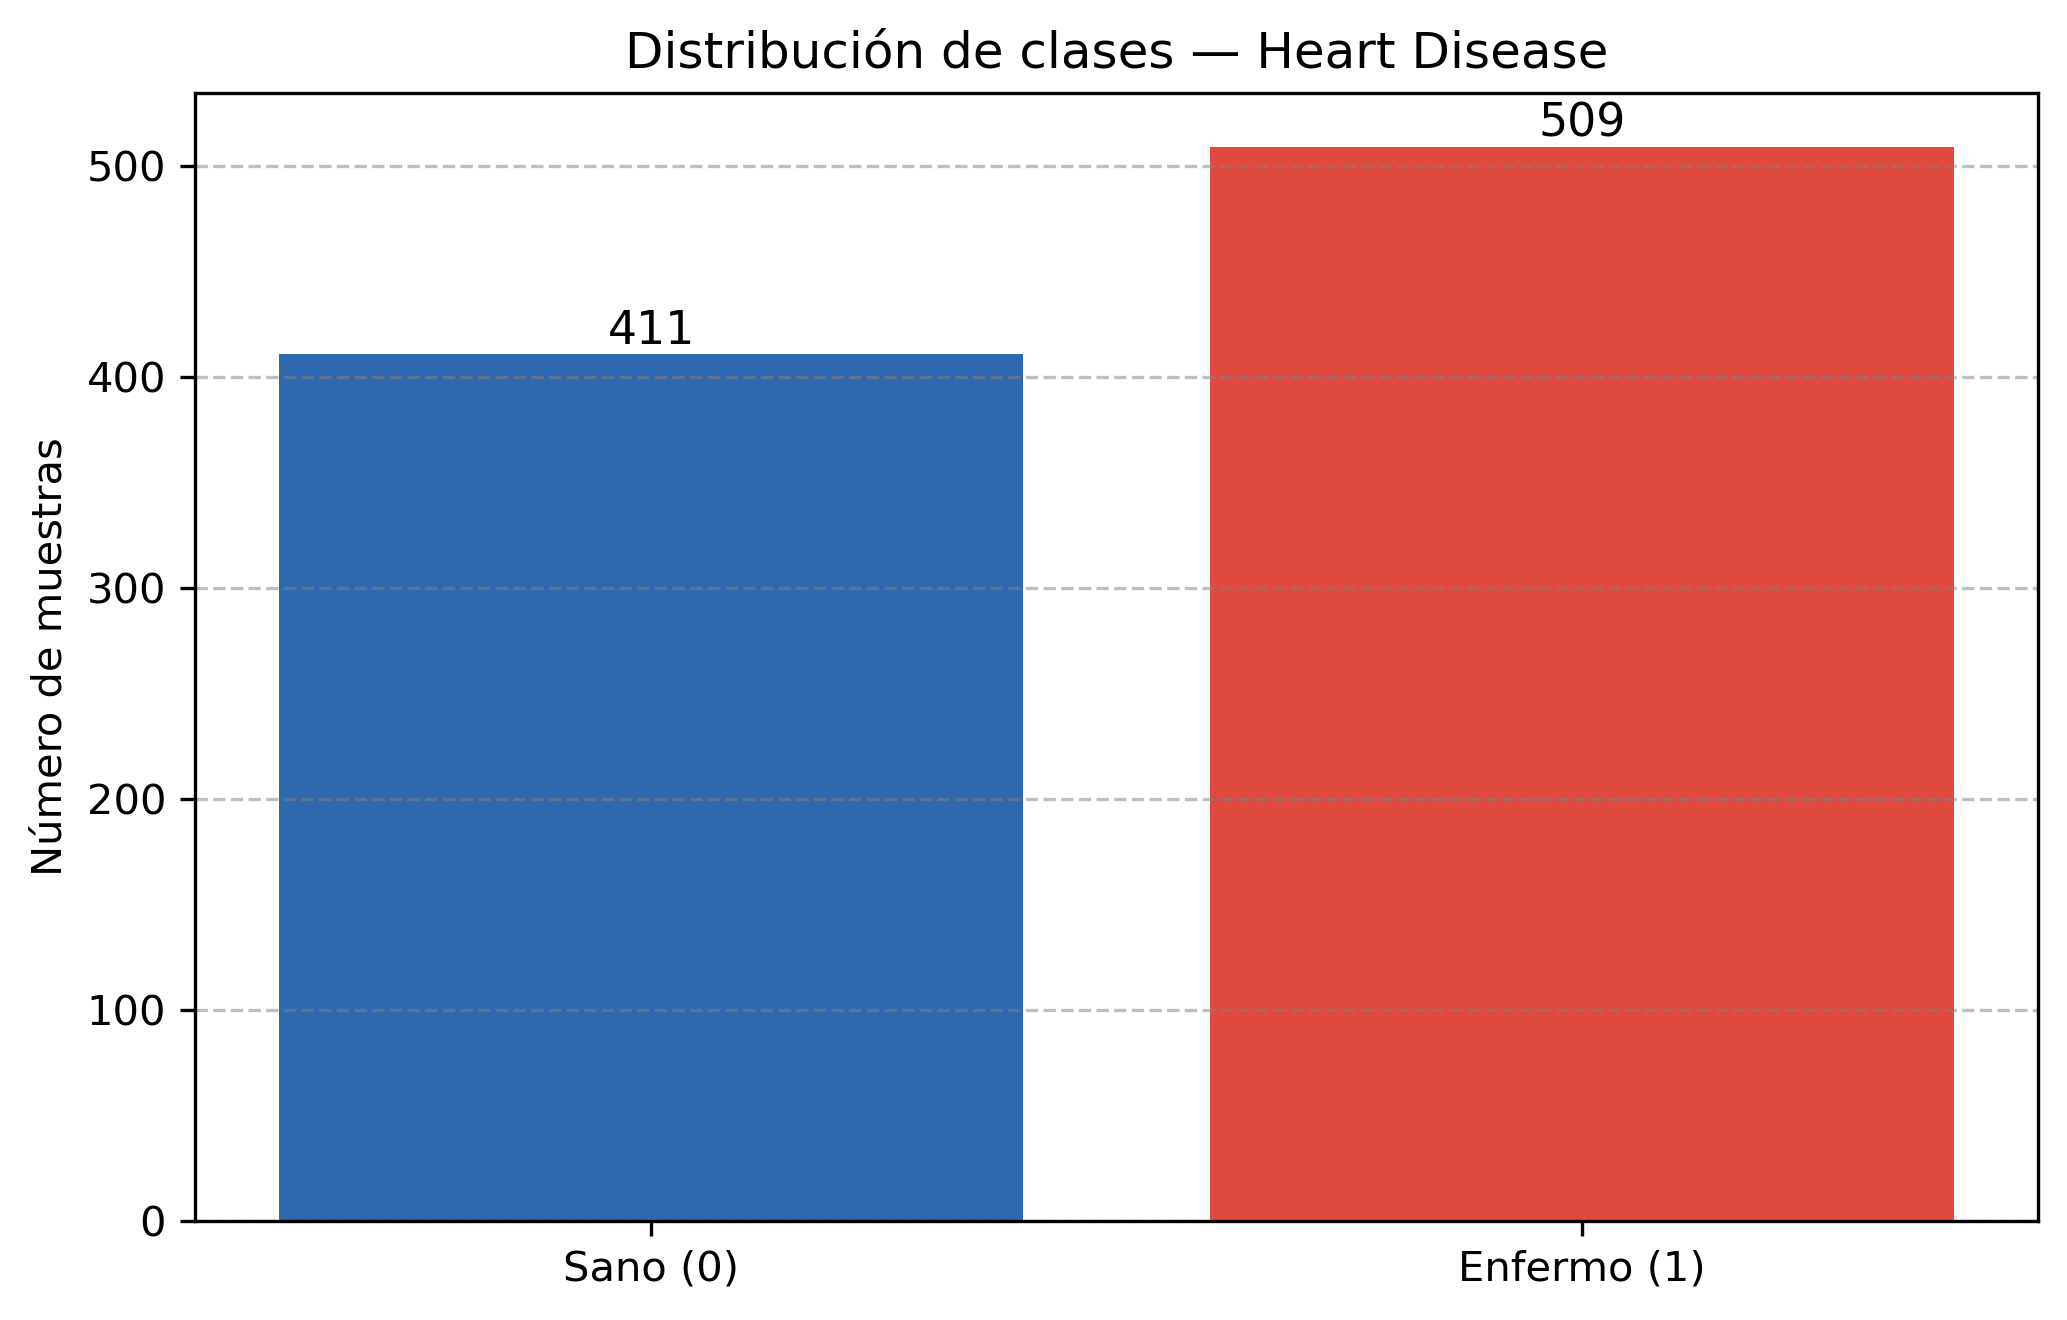
\includegraphics[width=0.65\textwidth]{Img/h_00_distribucion_clases.png}
    \caption{Distribución de clases tras la reformulación binaria de
        Heart Disease.}
    \label{fig:heart-distribucion}
\end{figure}

\begin{figure}[H]
    \centering
    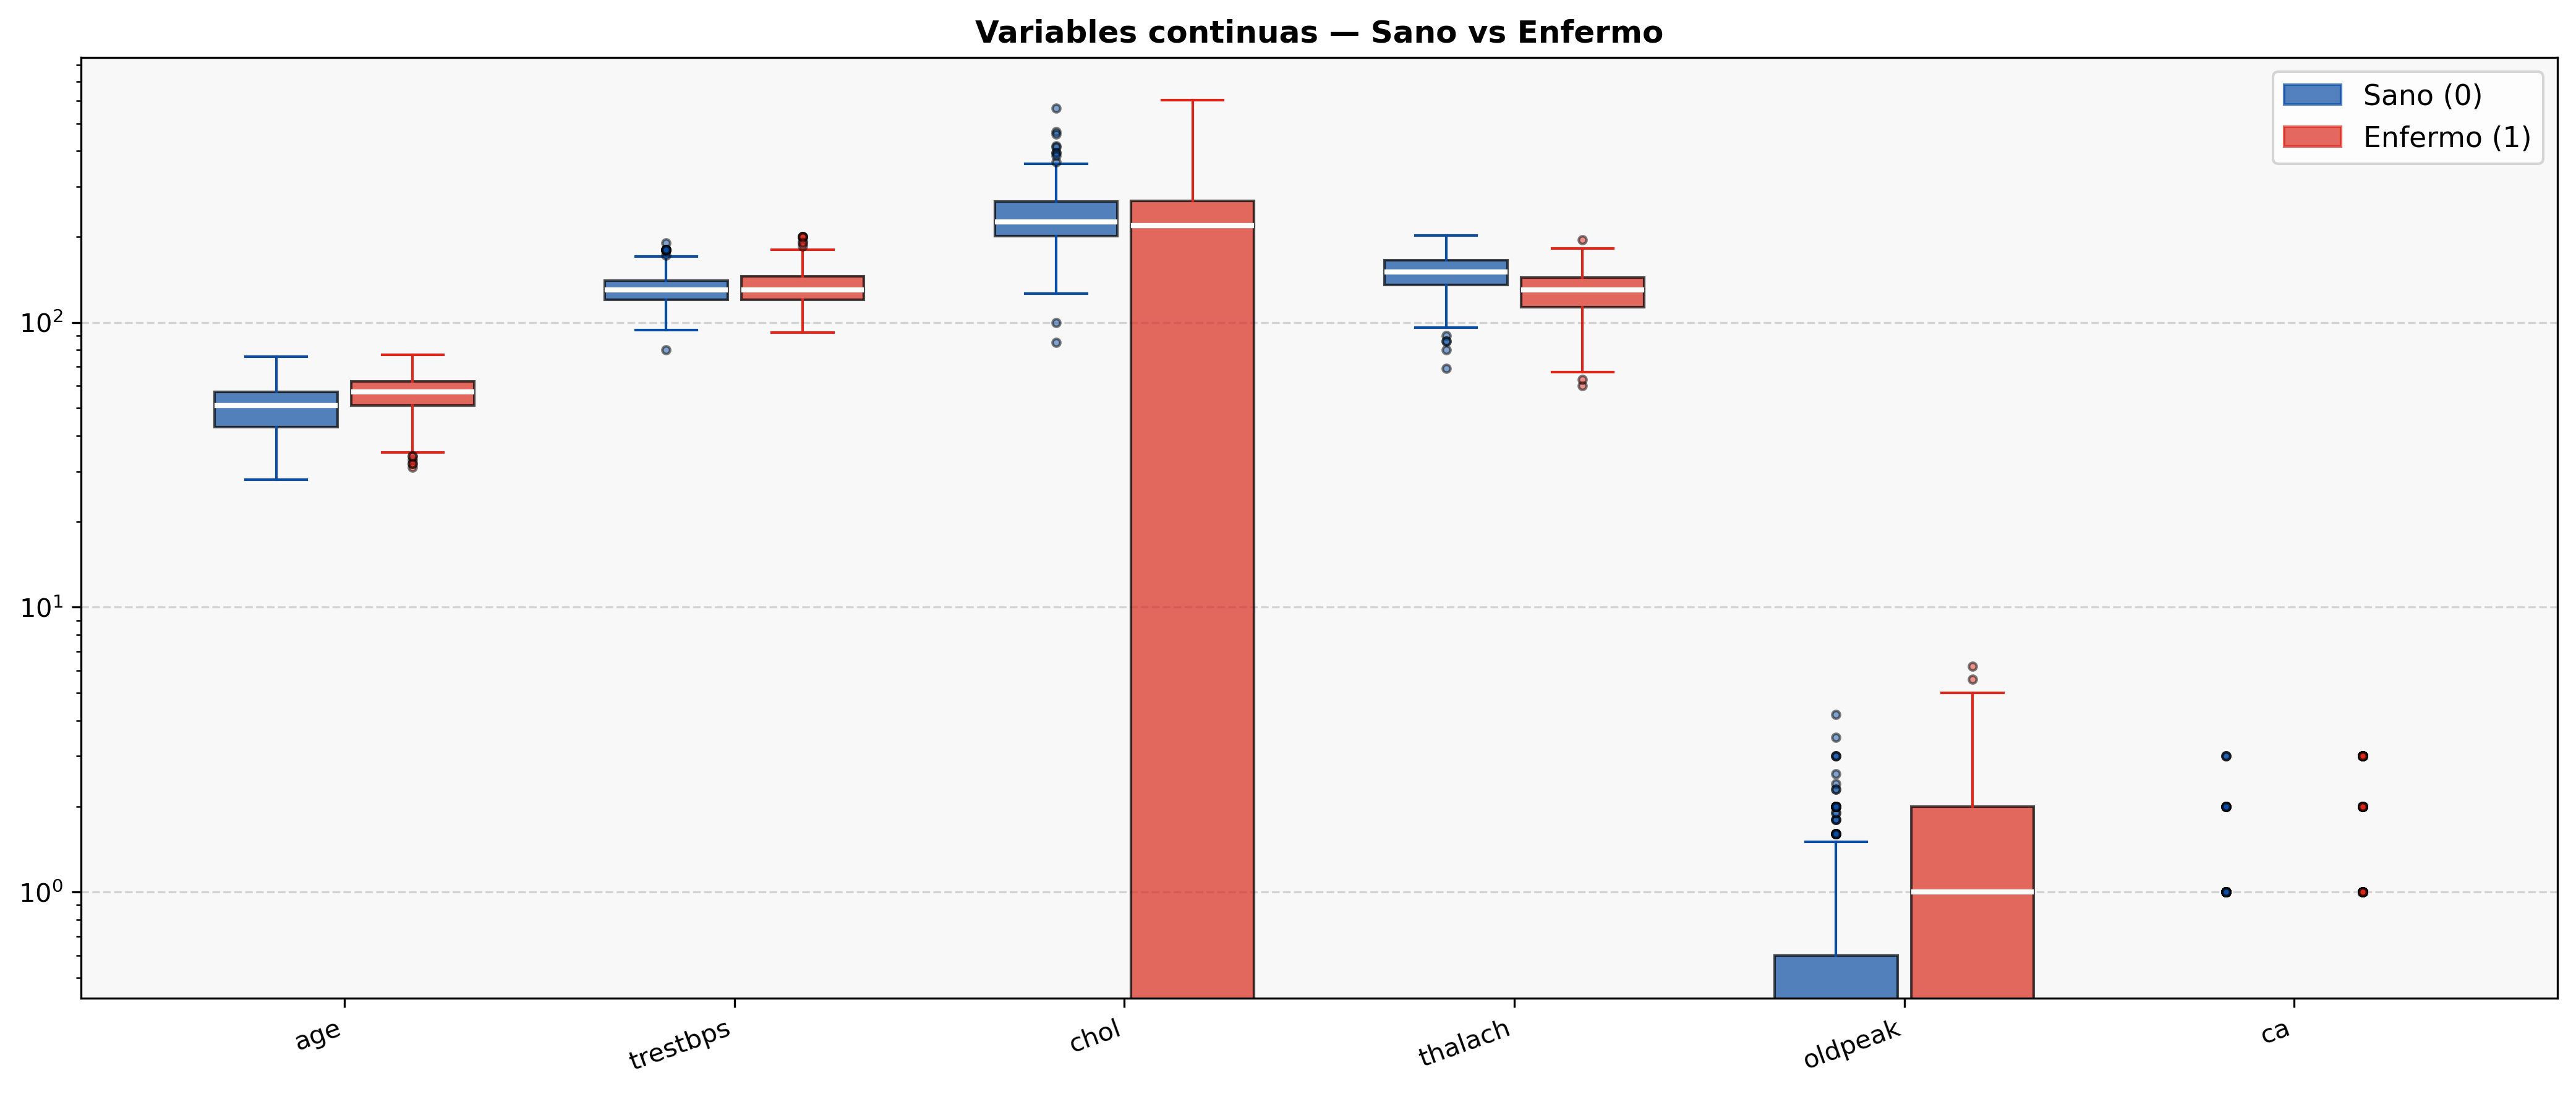
\includegraphics[width=1\textwidth]{Img/h_01_boxplot_continuas.png}
    \caption{\textit{Boxplots} comparativos de las variables continuas
        de Heart Disease, separados por clase.}
    \label{fig:heart-boxplots}
\end{figure}

Aunque varias variables muestran sesgos consistentes con el diagnóstico
---por ejemplo, los pacientes enfermos tienden a tener \texttt{thalach}
(frecuencia cardíaca máxima alcanzada) más baja y \texttt{oldpeak}
(depresión del ST inducida) más alta---, el solapamiento entre clases es
considerable. La detección de \textit{outliers} con IQR identificó 330
filas con al menos un valor extremo, principalmente en \texttt{chol}
(185 \textit{outliers}, $20.1\%$) y \texttt{ca} (128, $13.9\%$). Estos
valores se conservaron porque corresponden a casos clínicamente reales
(colesterol extremadamente alto, múltiples vasos afectados) y eliminarlos
sesgaría el modelo precisamente en la población más enferma.

\subsubsection*{Preprocesamiento, partición y SMOTE}

A diferencia del notebook de Cancer, aquí el escalado se ajustó
\textit{después} del \texttt{train\_test\_split} para evitar fuga de
información del conjunto de prueba. La partición $70/30$ produjo 644
muestras de entrenamiento y 276 de prueba. SMOTE se aplicó solo sobre
\textit{train}, llevando los conteos de 288 sanos / 356 enfermos a
356/356 (Figura~\ref{fig:heart-smote}).

\begin{figure}[H]
    \centering
    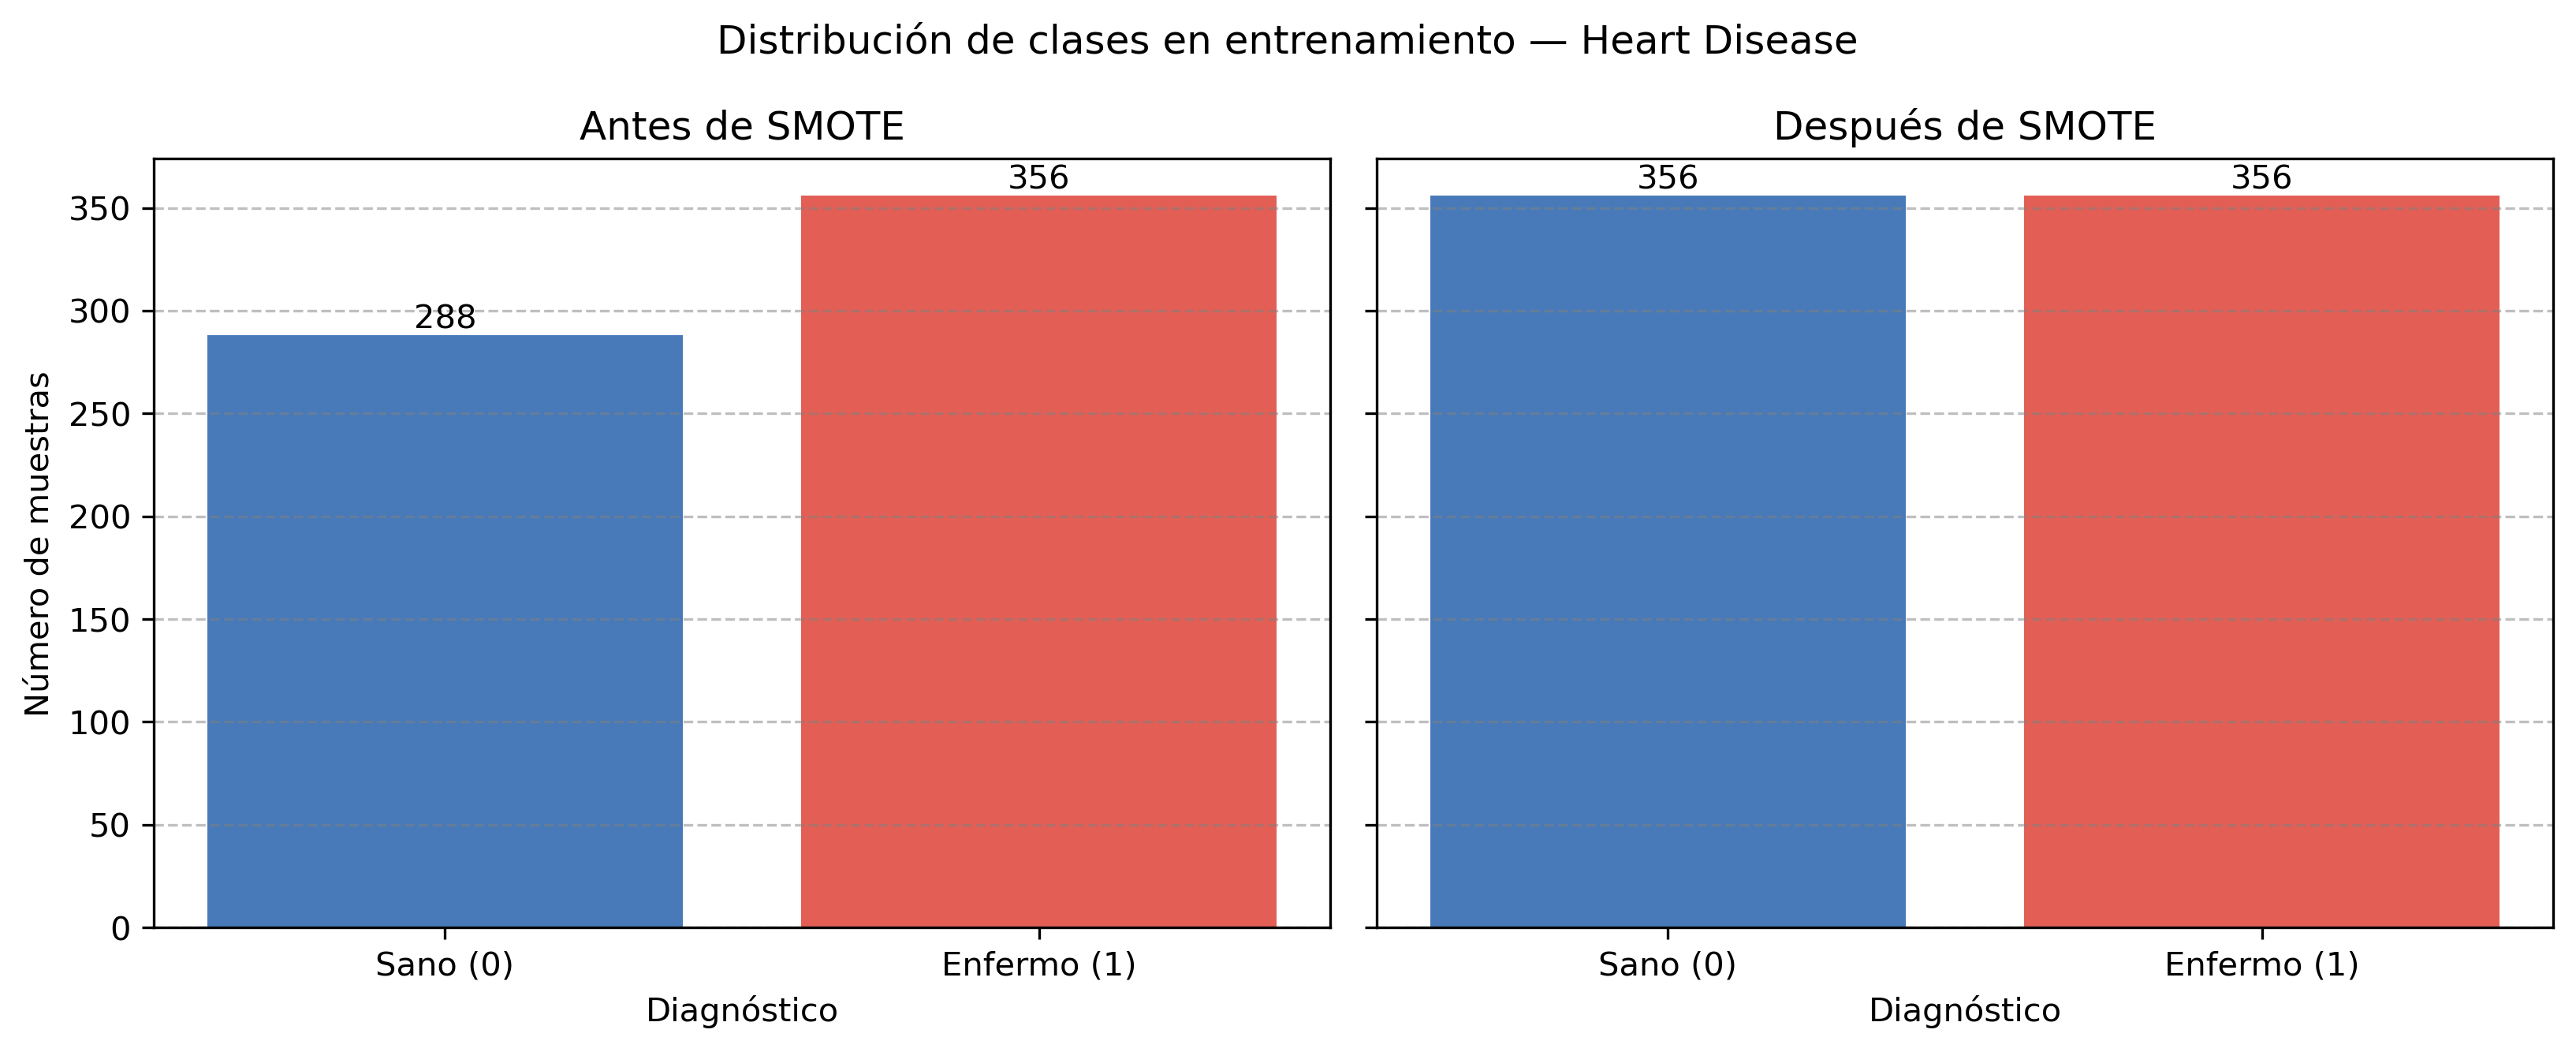
\includegraphics[width=0.85\textwidth]{Img/h_02_distribucion_smote.png}
    \caption{Distribución de clases en \textit{train} de Heart Disease
        antes y después de SMOTE.}
    \label{fig:heart-smote}
\end{figure}

\subsubsection*{Reducción de dimensionalidad}

PCA con \textit{Minka's MLE} seleccionó \textbf{11 componentes} y el
umbral del $95\%$ se alcanzó con \textbf{12} ---es decir, las 13
variables originales son prácticamente todas informativas y existe muy
poca redundancia--- (Figuras~\ref{fig:heart-var-mle} y
\ref{fig:heart-var-95}). Este es un comportamiento marcadamente
distinto del observado en Cancer, donde el $95\%$ se alcanzaba con tan
solo 10 de las 30 originales: en Heart Disease cada predictora aporta
información sustancial y la compresión es modesta.

\begin{figure}[H]
    \centering
    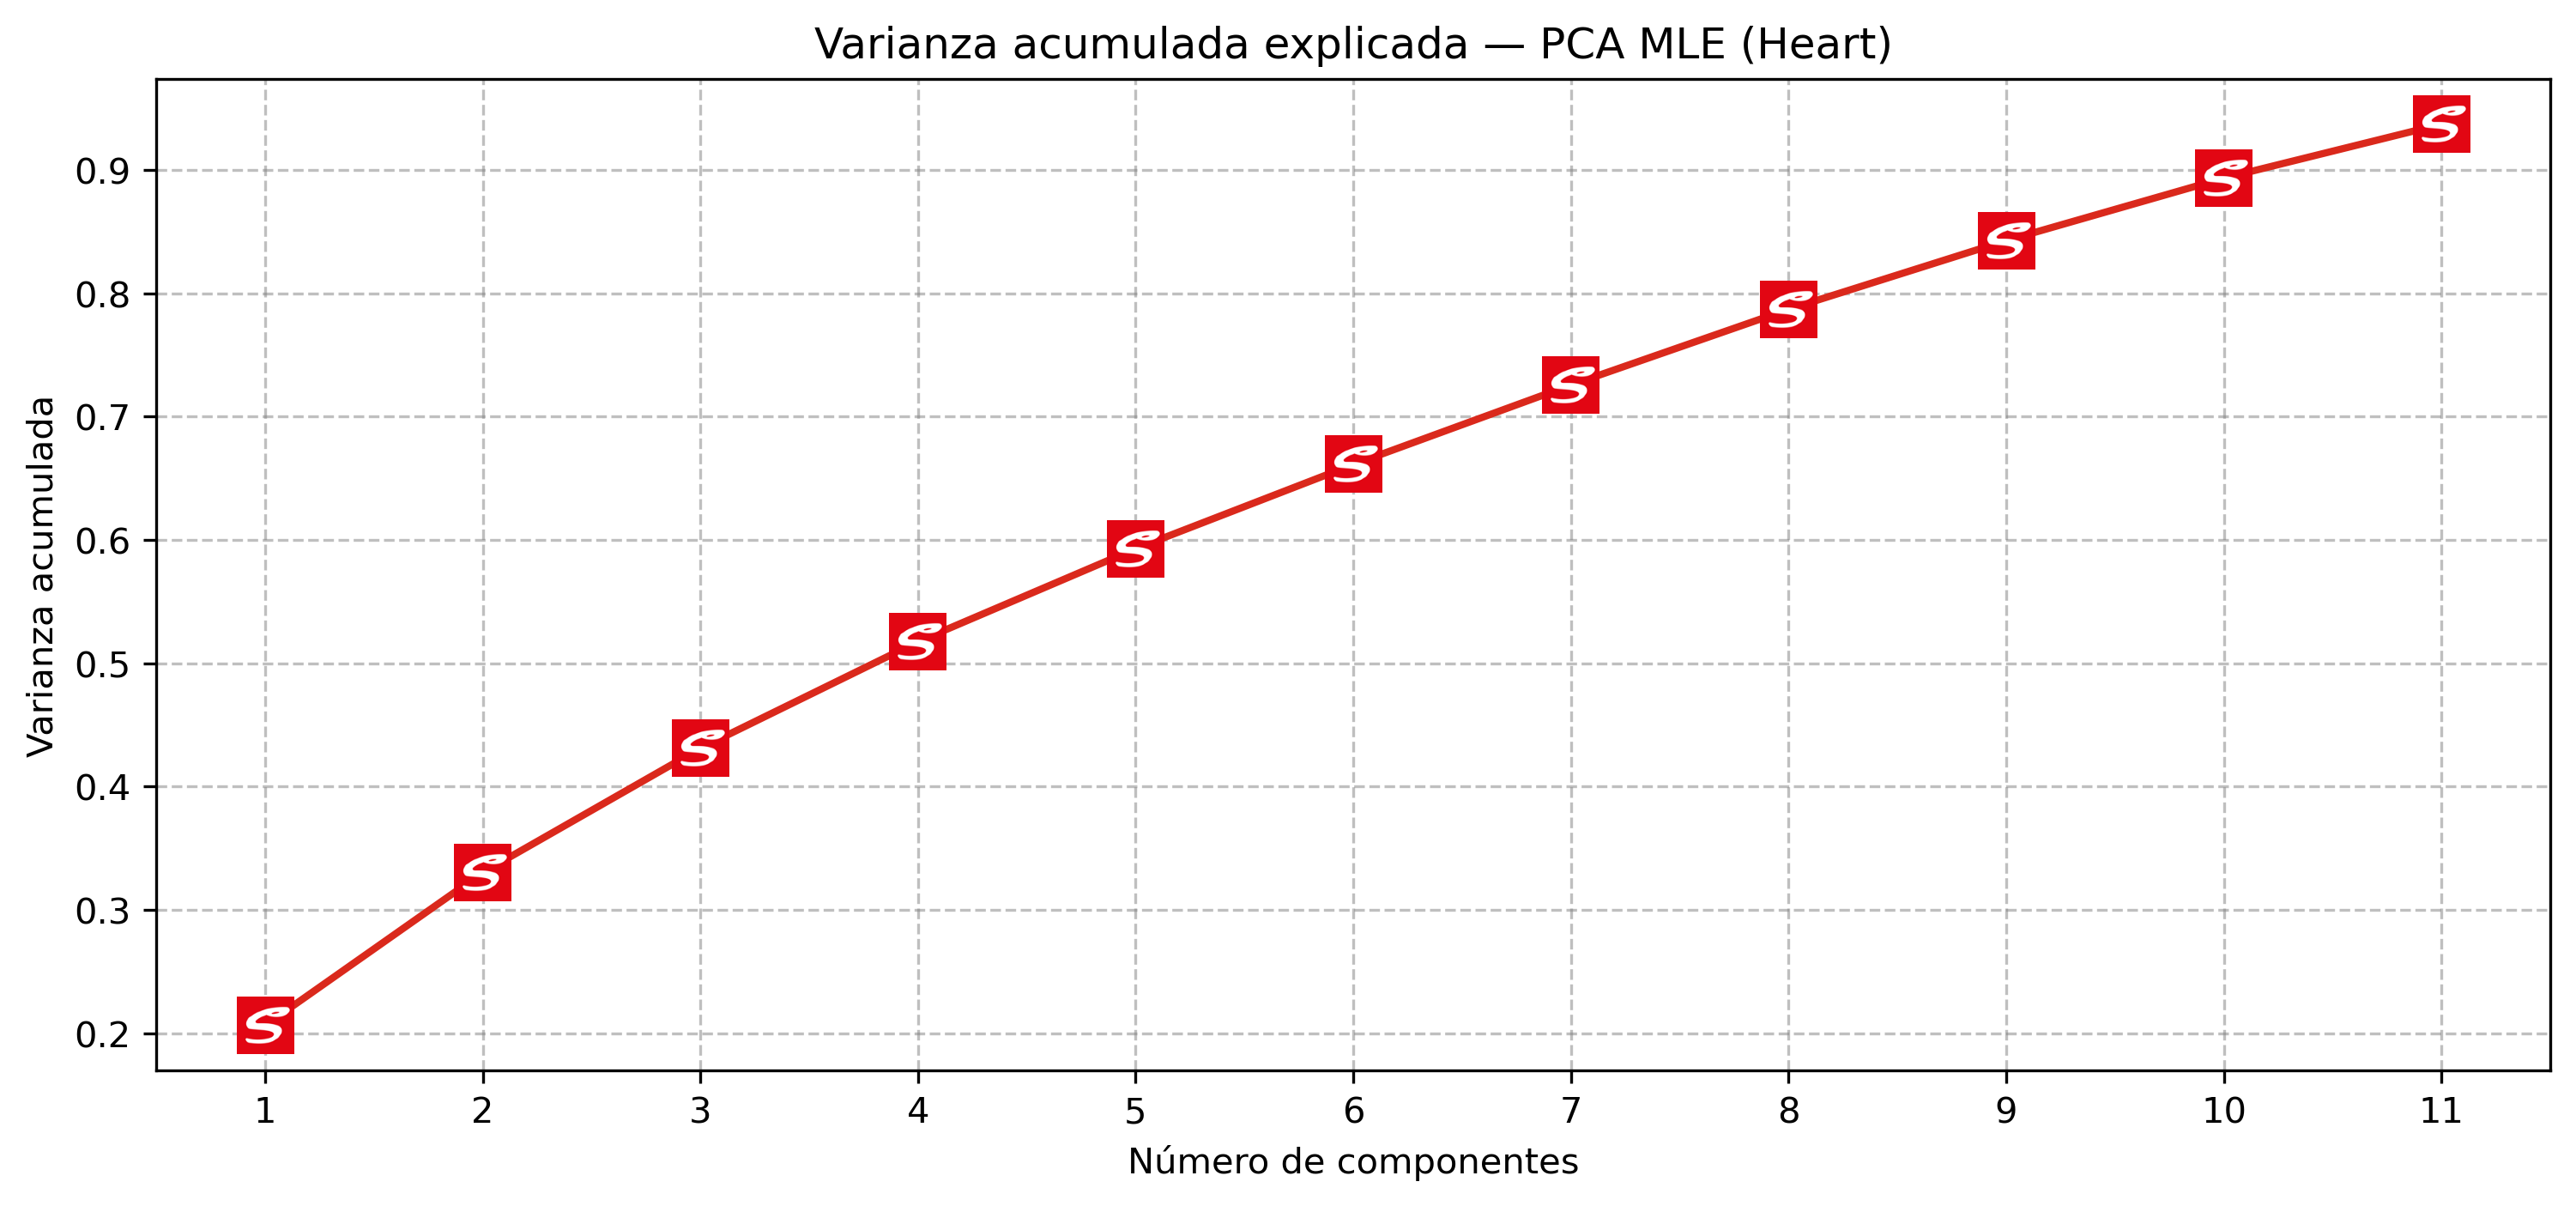
\includegraphics[width=0.95\textwidth]{Img/h_03_varianza_acumulada_mle.png}
    \caption{Varianza acumulada con PCA \textit{MLE} sobre Heart Disease
        (11 componentes seleccionados).}
    \label{fig:heart-var-mle}
\end{figure}

\begin{figure}[H]
    \centering
    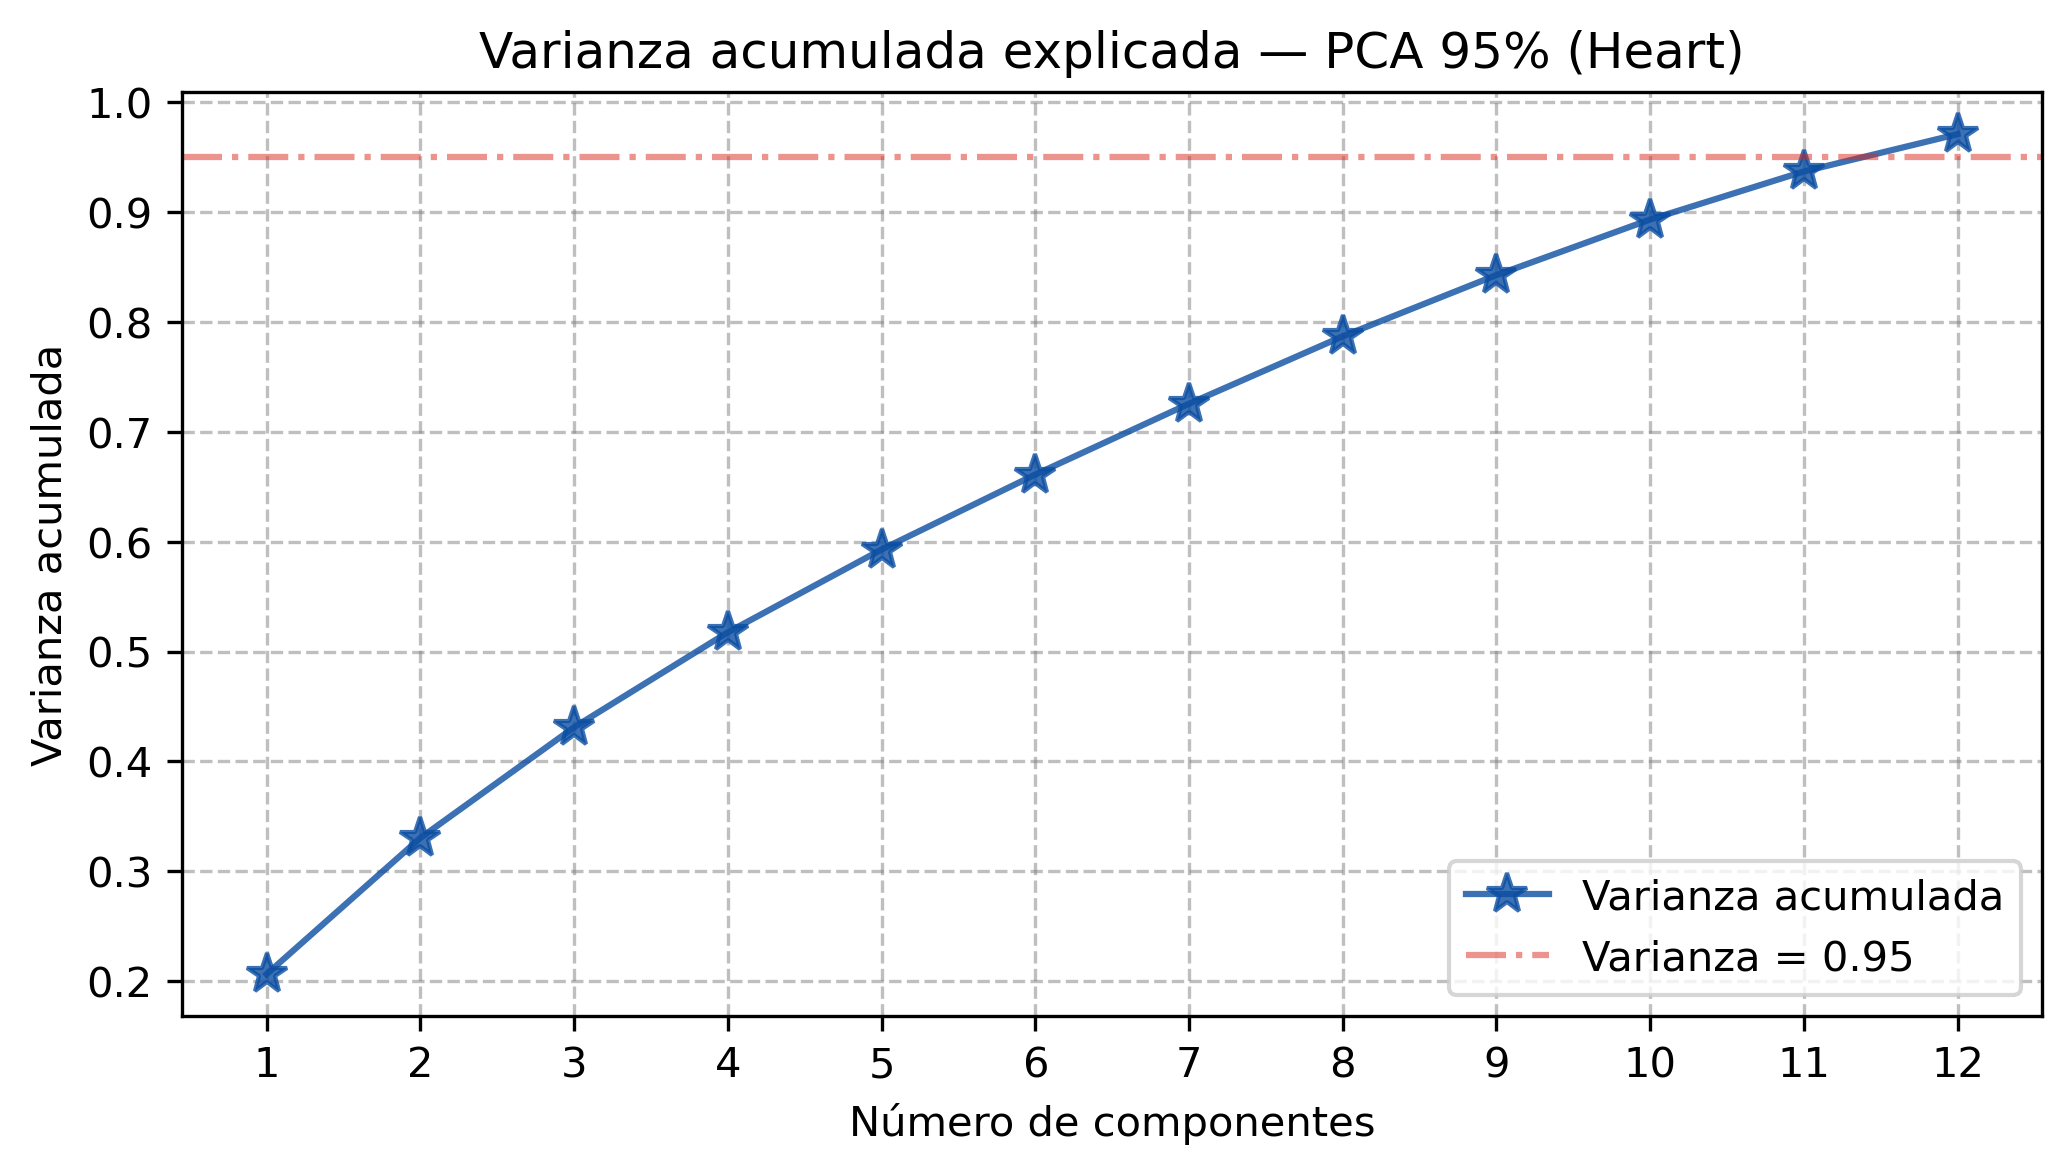
\includegraphics[width=0.85\textwidth]{Img/h_04_varianza_acumulada_var95.png}
    \caption{Varianza acumulada al fijar PCA con $95\%$: se requieren 12
        componentes.}
    \label{fig:heart-var-95}
\end{figure}

La proyección 2D de la Figura~\ref{fig:heart-pca-2d} evidencia el
contraste con Cancer: aquí las dos clases se solapan ampliamente. Esta
es la principal razón por la que las exactitudes de los modelos sobre
Heart Disease ($\sim 0.84$) son notablemente menores que sobre Cancer
($\sim 0.97$): el problema es intrínsecamente más difícil.

\begin{figure}[H]
    \centering
    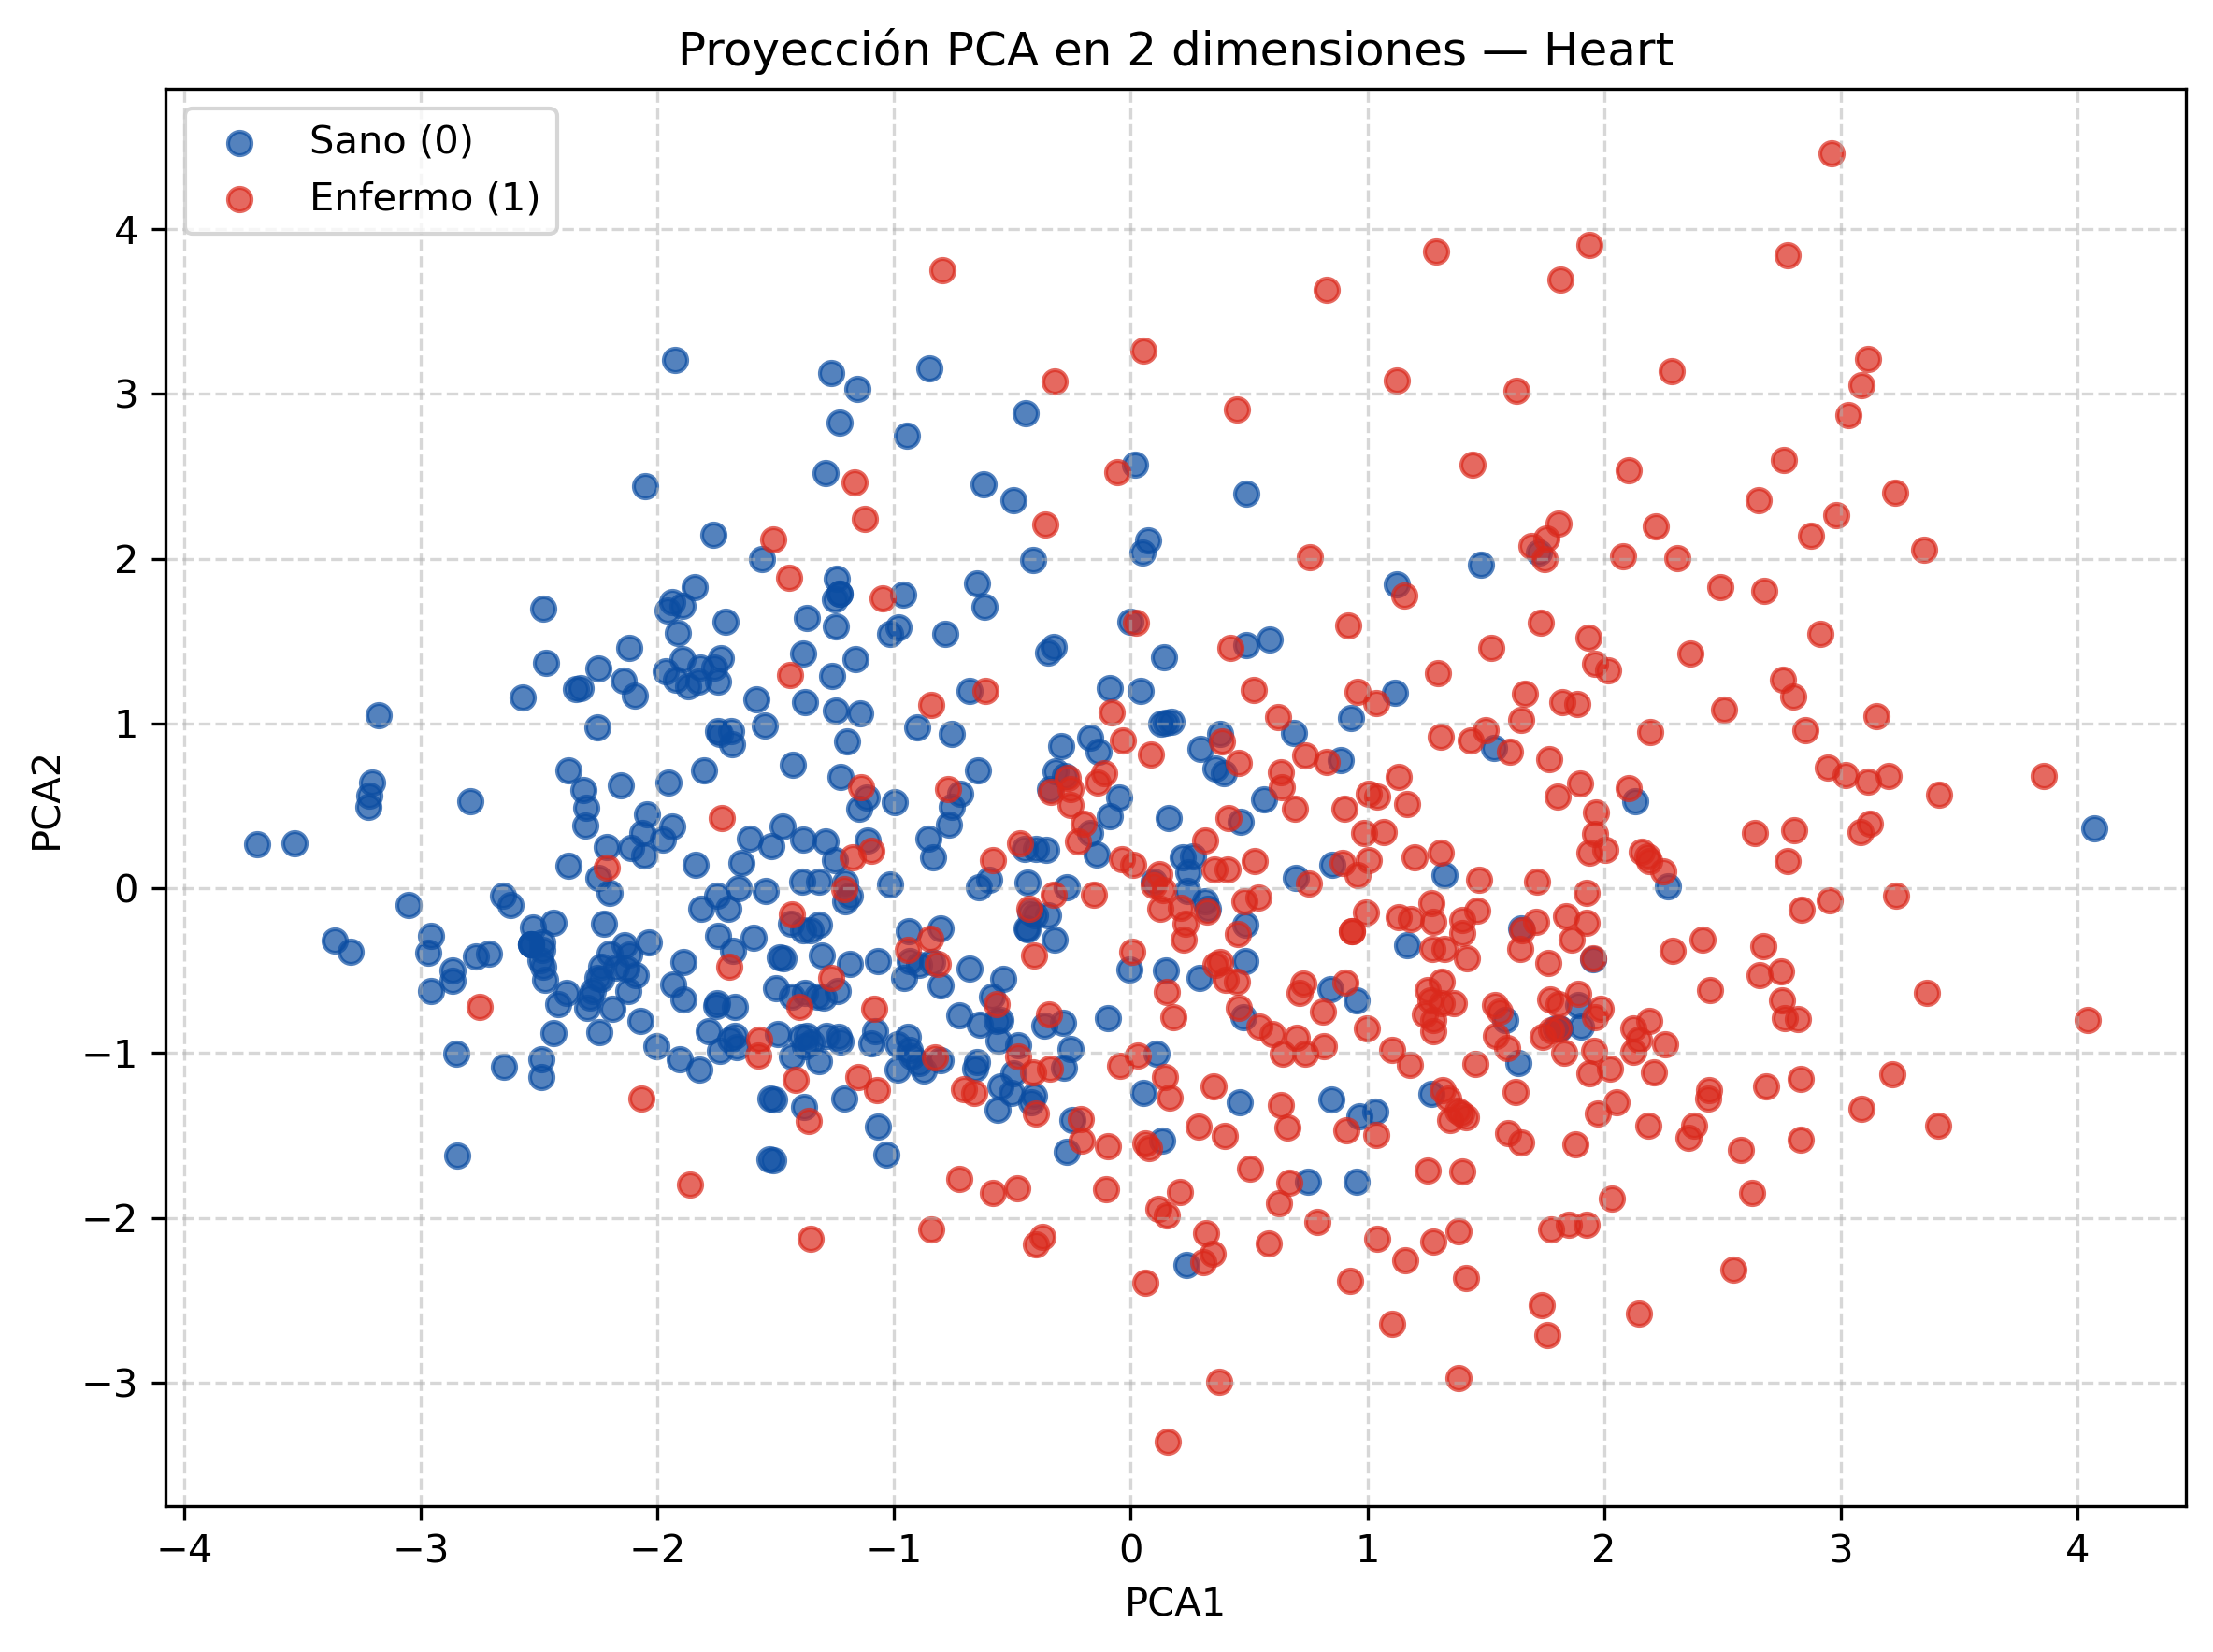
\includegraphics[width=0.80\textwidth]{Img/h_05_pca_2d.png}
    \caption{Proyección 2D de PCA sobre Heart Disease. El solapamiento
        entre Sano y Enfermo es considerable.}
    \label{fig:heart-pca-2d}
\end{figure}

\subsubsection*{Búsqueda en cuadrícula y resultados}

Se aplicó el mismo esquema de \texttt{GridSearchCV} con CV de 5
\textit{folds}. Los mejores resultados aparecen en la
Tabla~\ref{tab:heart-resultados}.

\begin{table}[H]
    \centering
    \rowcolors{2}{rowgray}{white}
    \begin{tabular}{lccccc}
        \toprule
        \rowcolor{headerblue}
        \textcolor{headertext}{\textbf{Modelo}}                  &
        \textcolor{headertext}{\textbf{Mejores hiperparámetros}} &
        \textcolor{headertext}{\textbf{CV Acc.}}                 &
        \textcolor{headertext}{\textbf{Test Acc.}}               &
        \textcolor{headertext}{\textbf{Recall}}                  &
        \textcolor{headertext}{\textbf{F1}}                                                                                                                                            \\
        \midrule
        KNN                                                      & $k=7$, \textit{distance}, manhattan & $0.8217$          & $\mathbf{0.8442}$ & $0.8627$          & $\mathbf{0.8599}$ \\
        Árbol de Decisión                                        & gini, depth$=5$, split$=5$          & $0.7880$          & $0.7536$          & $0.7320$          & $0.7671$          \\
        SVM                                                      & RBF, $C=1$, $\gamma=$scale          & $\mathbf{0.8400}$ & $0.8225$          & $\mathbf{0.8693}$ & $0.8444$          \\
        \bottomrule
    \end{tabular}
    \caption{Resultados de los tres clasificadores sobre Heart Disease.}
    \label{tab:heart-resultados}
\end{table}

A diferencia de Cancer, aquí gana \textbf{KNN} en exactitud sobre el
conjunto de prueba ($0.8442$), aunque el SVM con kernel RBF lo supera
ligeramente en \textit{recall} ($0.8693$ vs $0.8627$). El árbol queda
claramente por debajo, lo que ya anticipaba el bajo desempeño esperable
de un único árbol cuando las clases están entrelazadas y las divisiones
ortogonales no alcanzan a capturar la frontera real. La
Figura~\ref{fig:heart-confusion} muestra las matrices de confusión.

\begin{figure}[H]
    \centering
    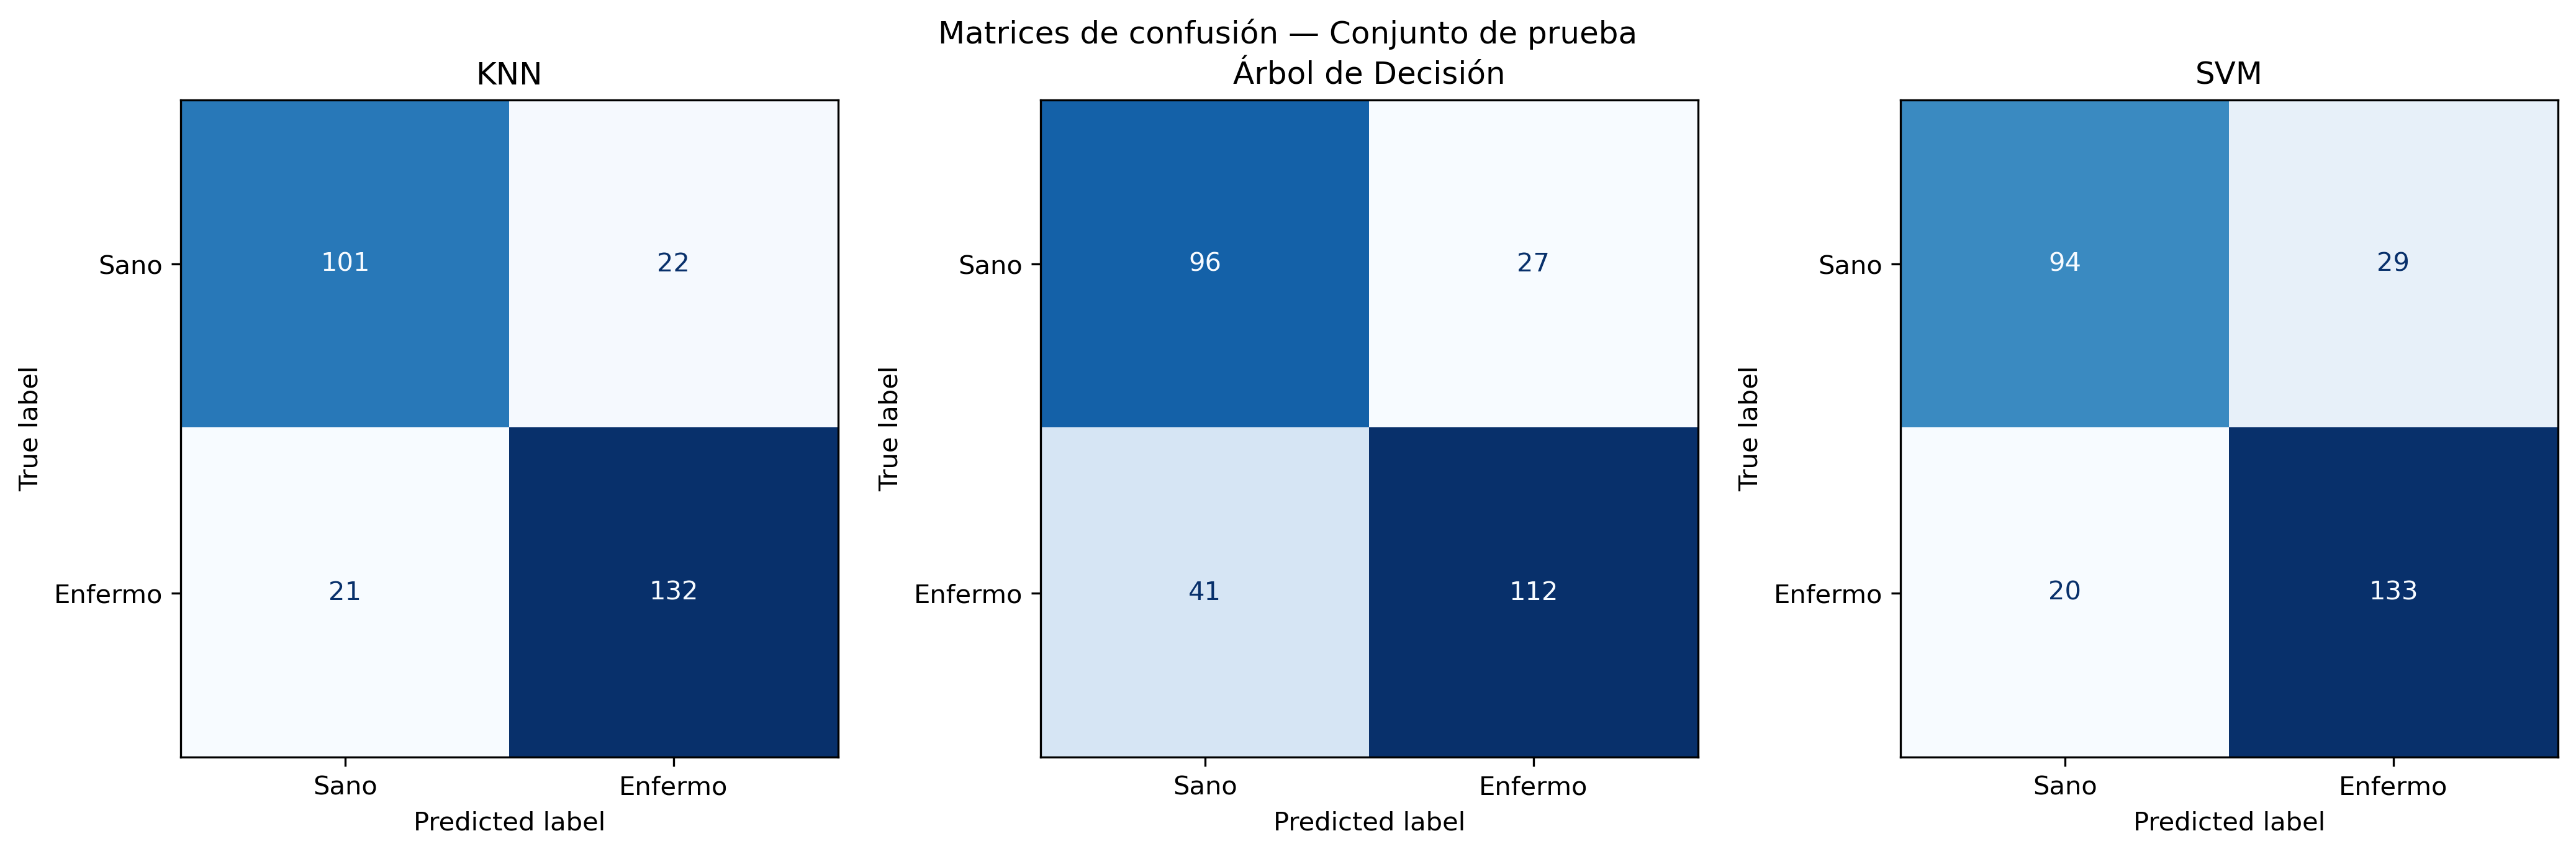
\includegraphics[width=1\textwidth]{Img/h_06_matrices_confusion.png}
    \caption{Matrices de confusión sobre el conjunto de prueba de Heart
        Disease.}
    \label{fig:heart-confusion}
\end{figure}

\subsubsection*{Fronteras de decisión en PCA 2D}

La Figura~\ref{fig:heart-fronteras} muestra las fronteras de los tres
modelos entrenados sobre las dos primeras componentes principales.
Comparadas con las de Cancer, las fronteras son mucho menos definidas:
los puntos de ambas clases se entremezclan y obligan a cada algoritmo a
producir regiones complejas y poco confiables fuera de las zonas más
densamente pobladas. Esta visualización ilustra por qué la exactitud no
puede ser tan alta como en Cancer y por qué el árbol ---que carece de la
flexibilidad geométrica del SVM-RBF y de la localidad del KNN--- es el
que más sufre.

\begin{figure}[H]
    \centering
    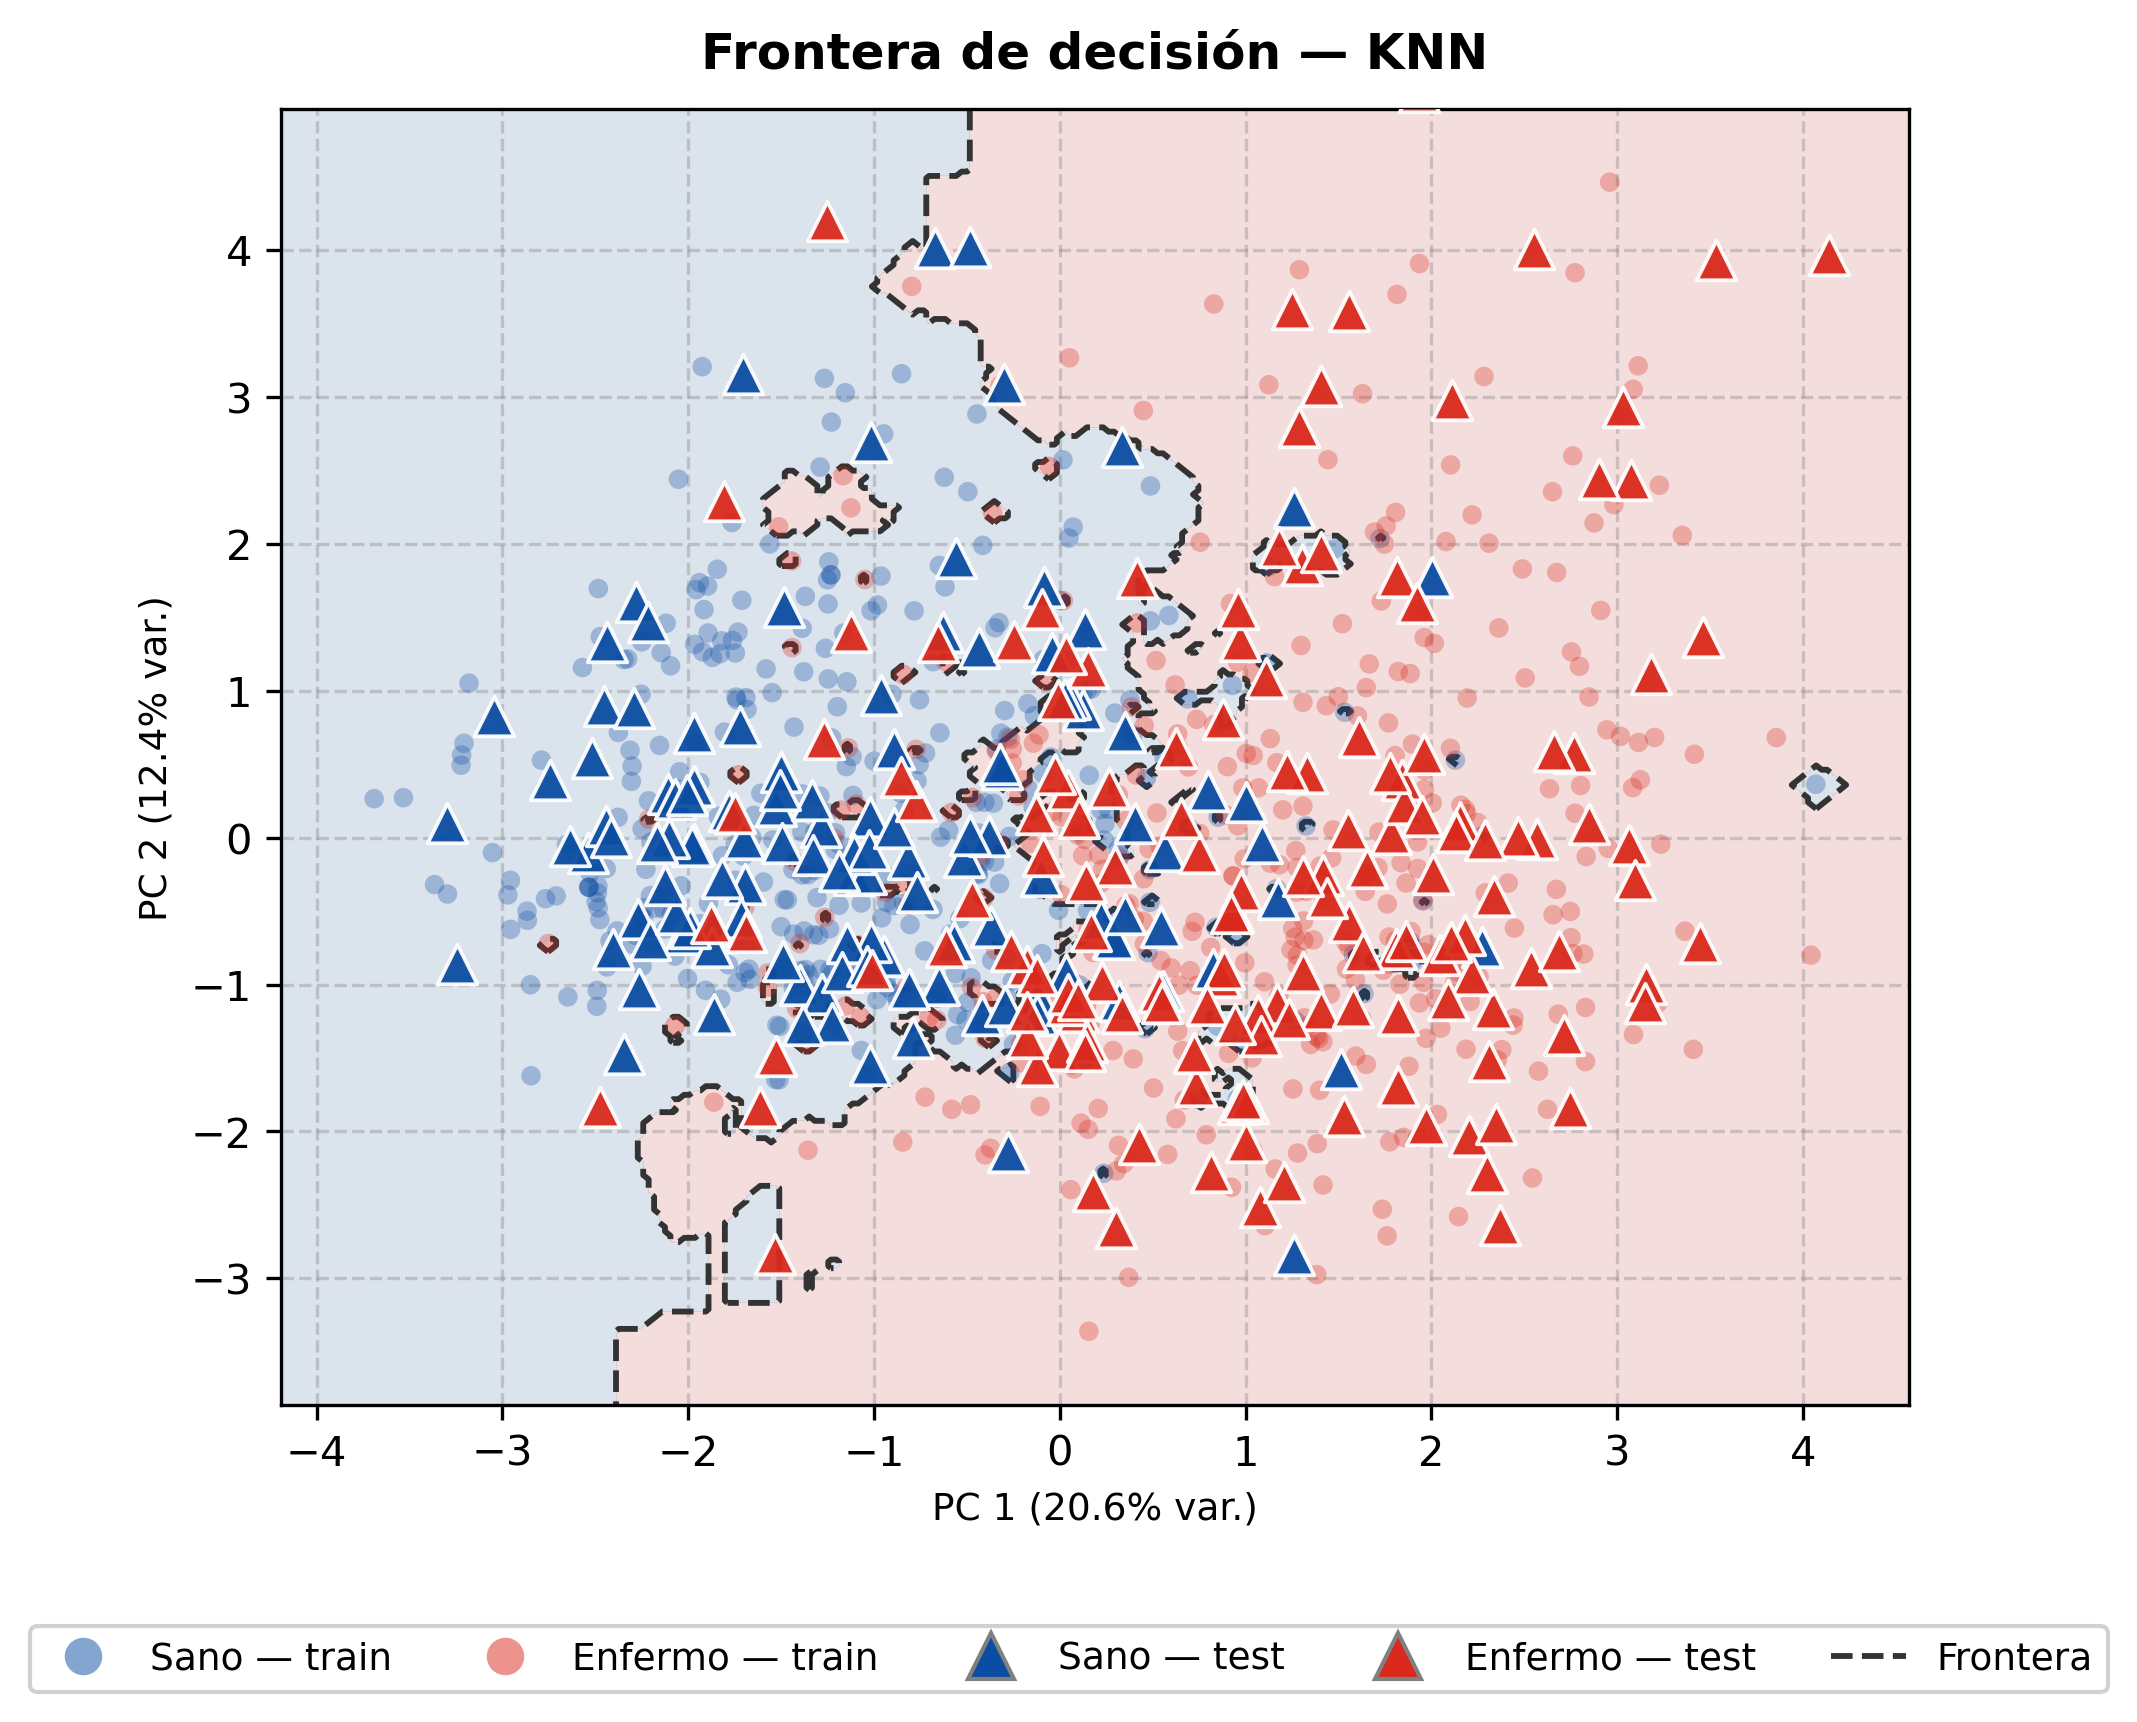
\includegraphics[width=0.49\textwidth]{Img/h_07a_frontera_knn.png}
    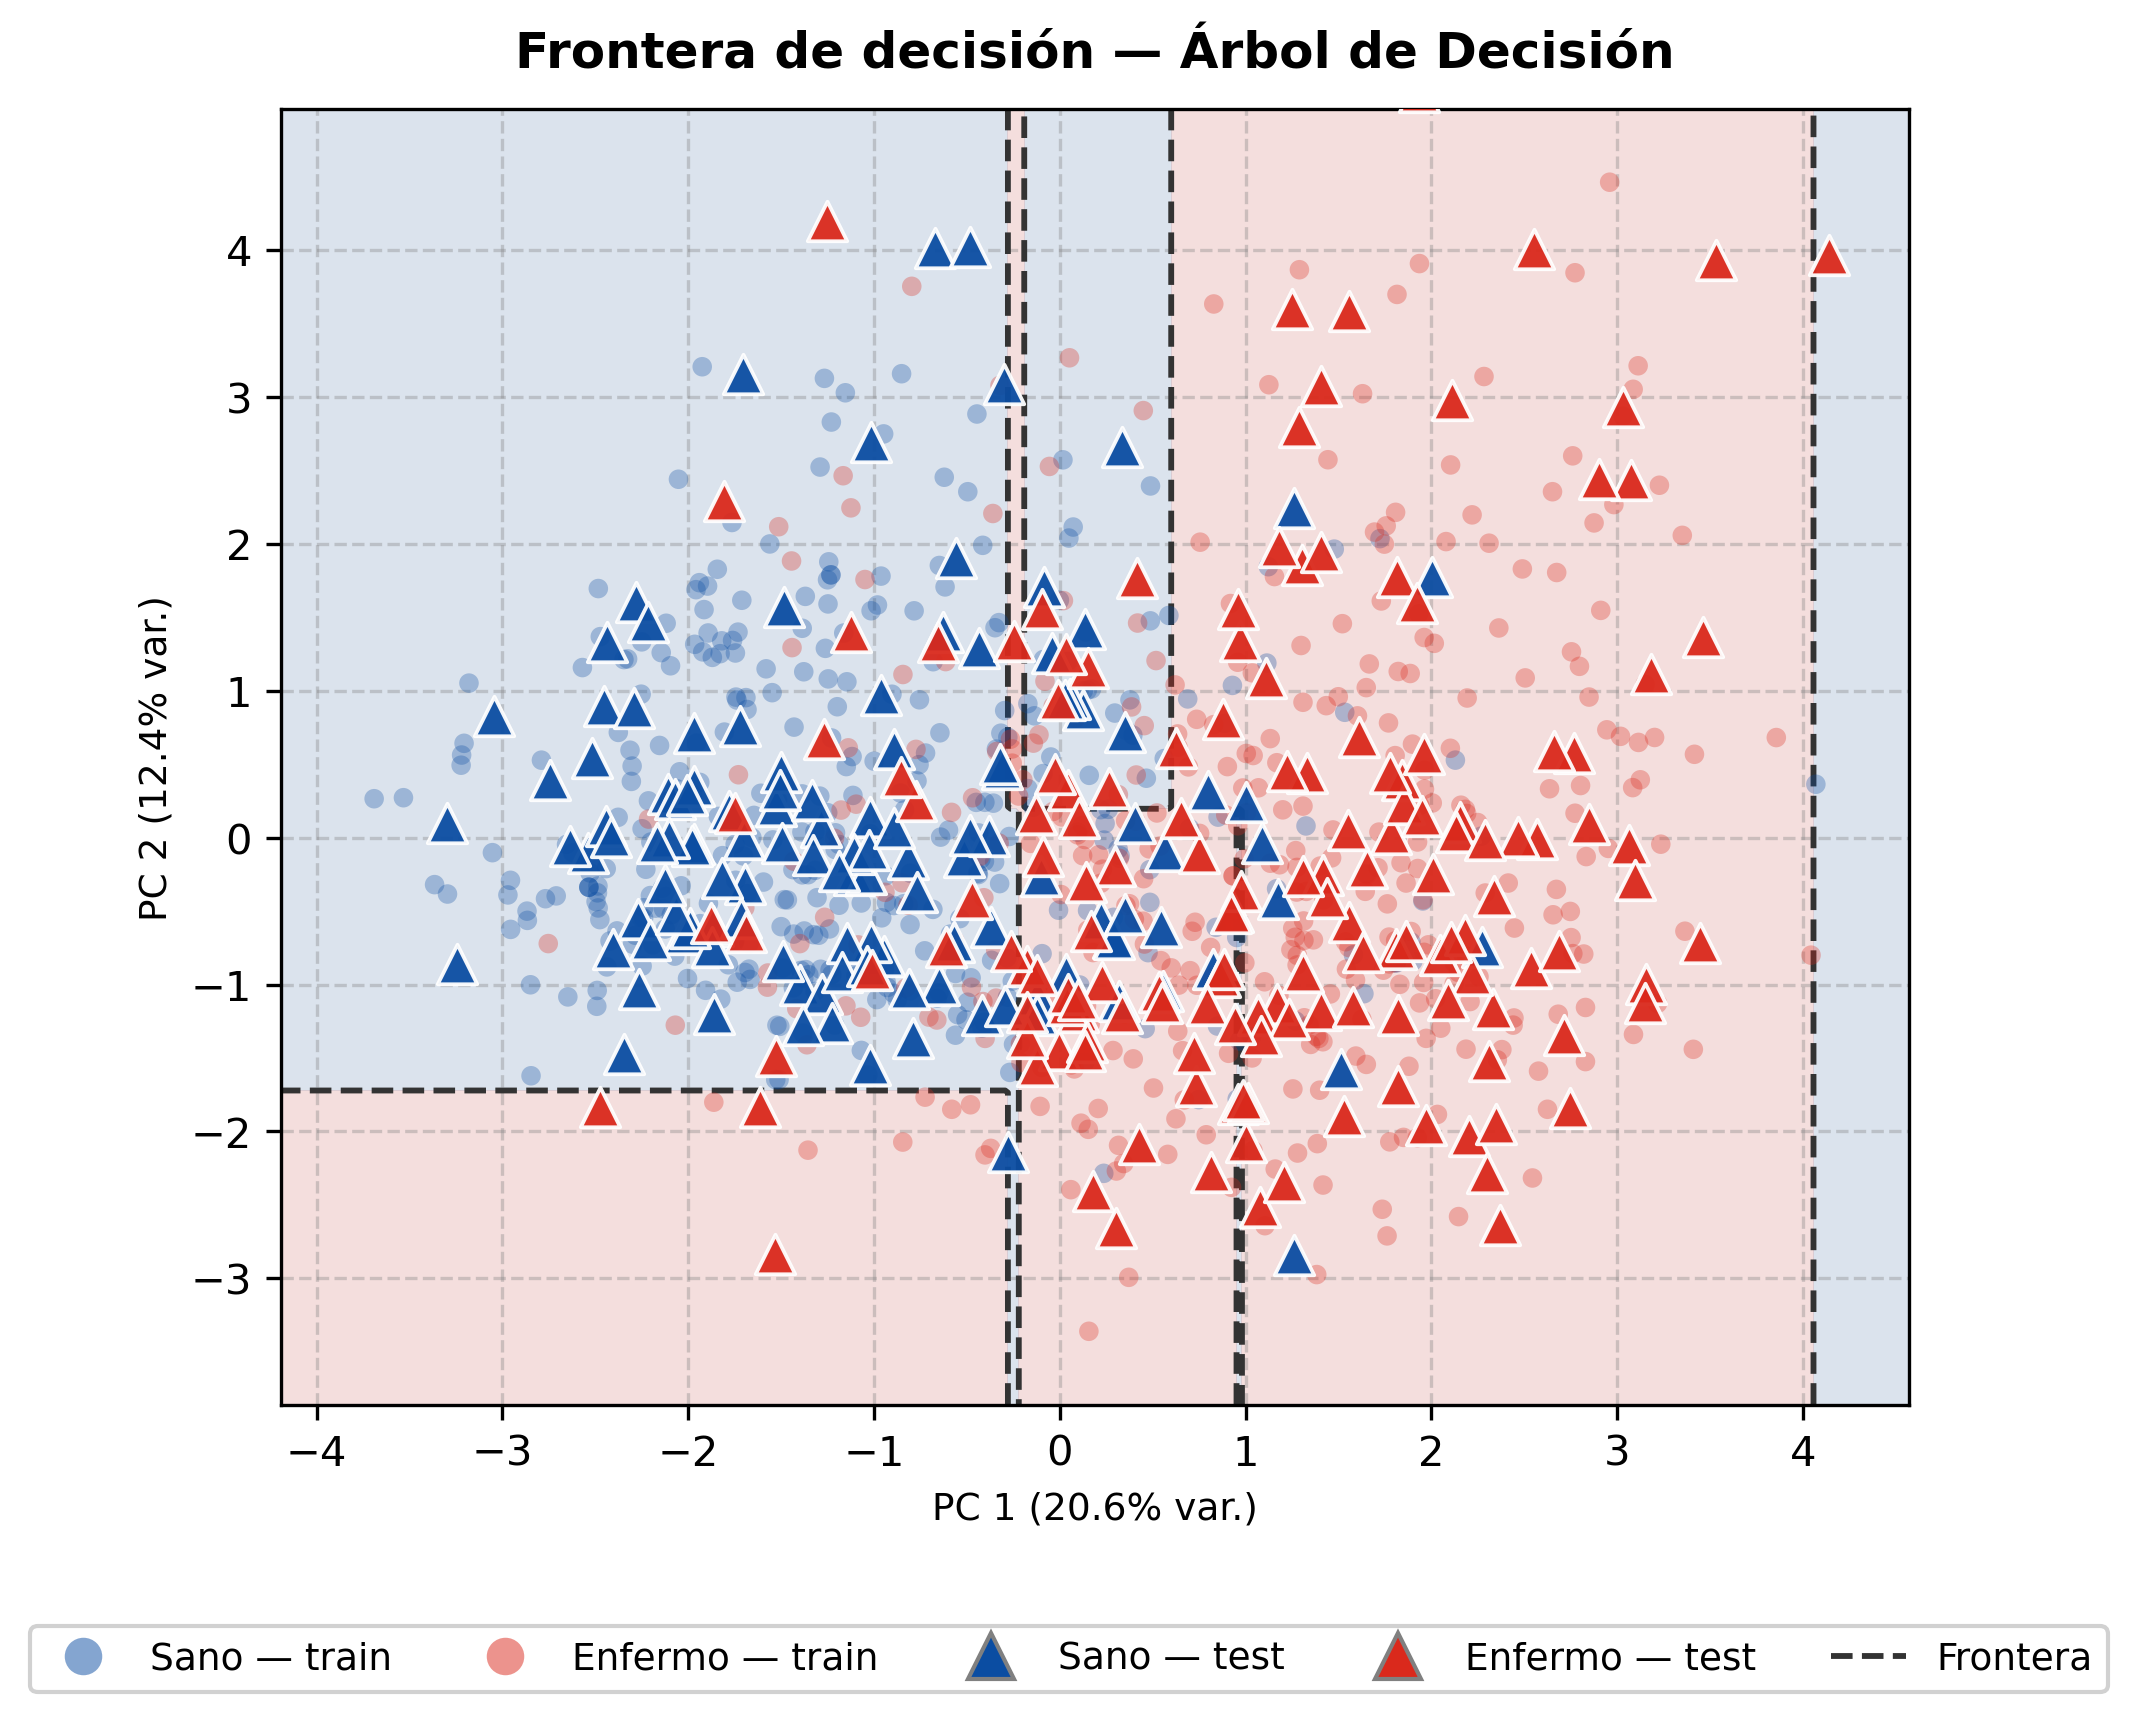
\includegraphics[width=0.49\textwidth]{Img/h_07b_frontera_arbol.png}
    \\[2mm]
    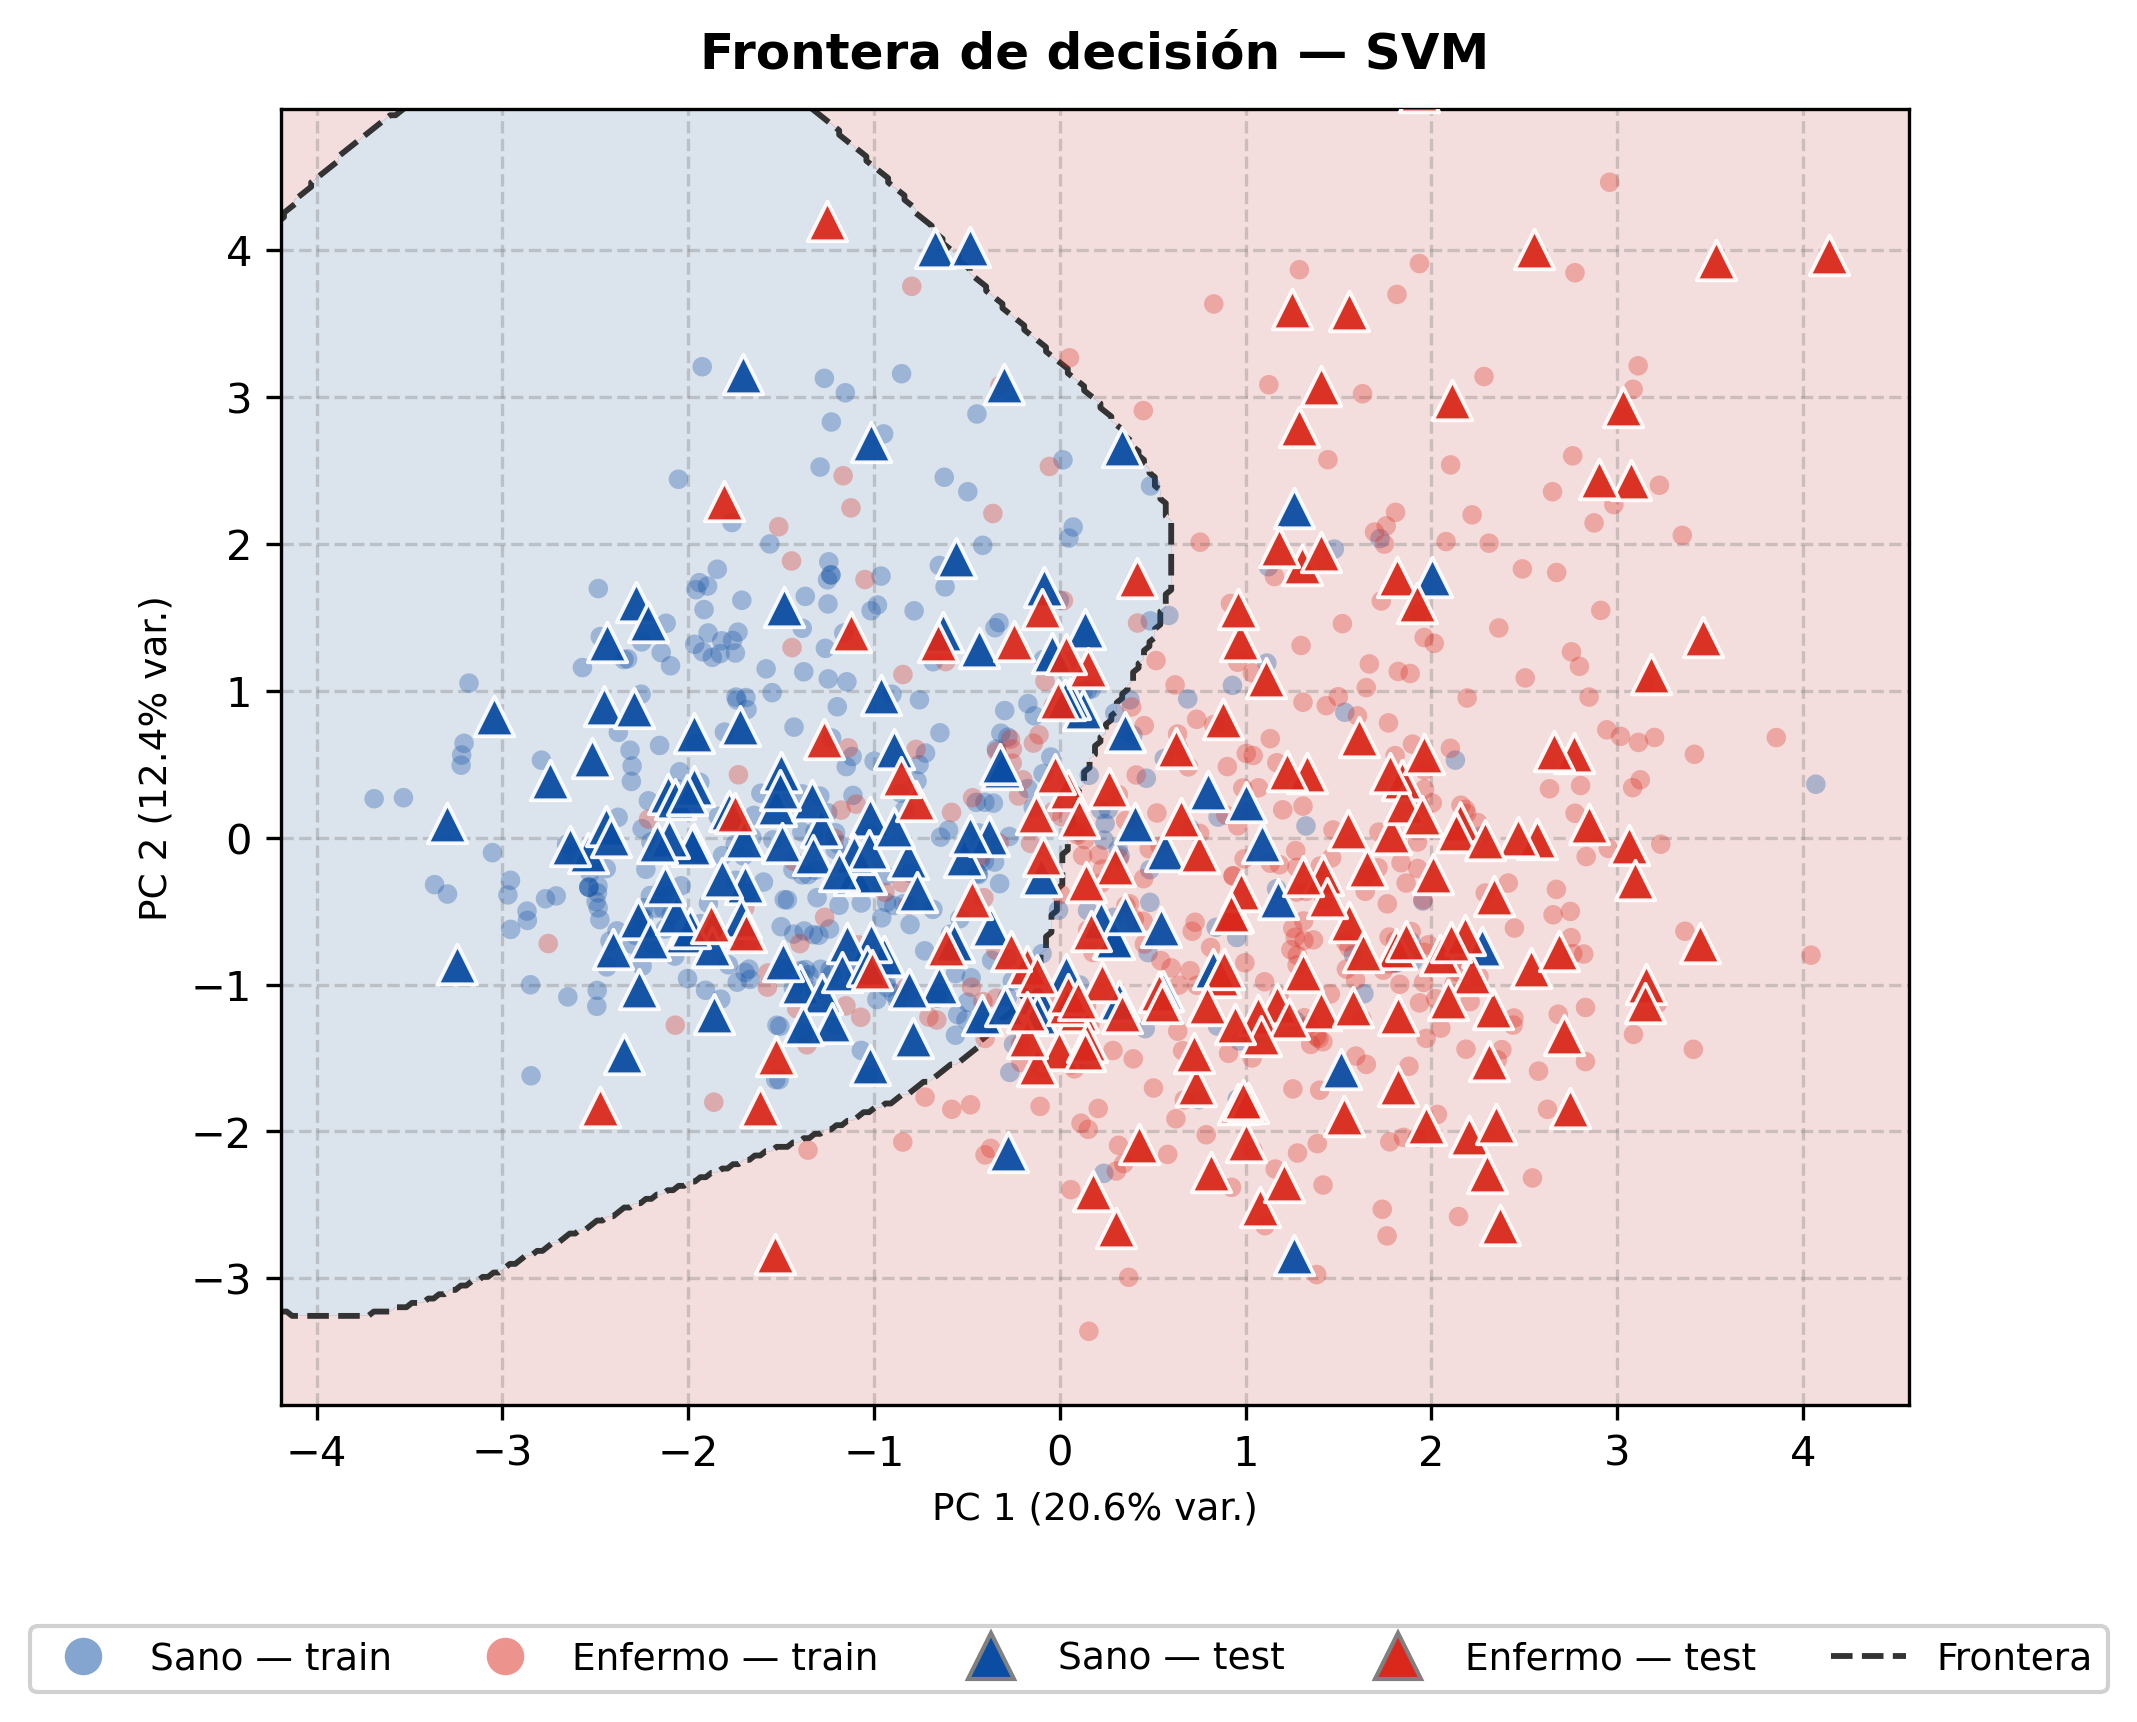
\includegraphics[width=0.49\textwidth]{Img/h_07c_frontera_svm.png}
    \caption{Fronteras de decisión en PCA 2D para Heart Disease: KNN
        (arriba izquierda), árbol (arriba derecha) y SVM-RBF (abajo).}
    \label{fig:heart-fronteras}
\end{figure}

\subsubsection*{Árbol de decisión}

El árbol entrenado con los mejores hiperparámetros se presenta en la
Figura~\ref{fig:heart-arbol}. El nodo raíz divide por \texttt{cp} (tipo
de dolor torácico), lo cual es clínicamente esperable porque es uno de
los predictores más informativos del riesgo cardíaco. Subsiguientes
divisiones involucran \texttt{thal}, \texttt{ca} y \texttt{oldpeak},
todas variables ya identificadas en la literatura como fuertemente
asociadas a la presencia de enfermedad coronaria.

\begin{figure}[H]
    \centering
    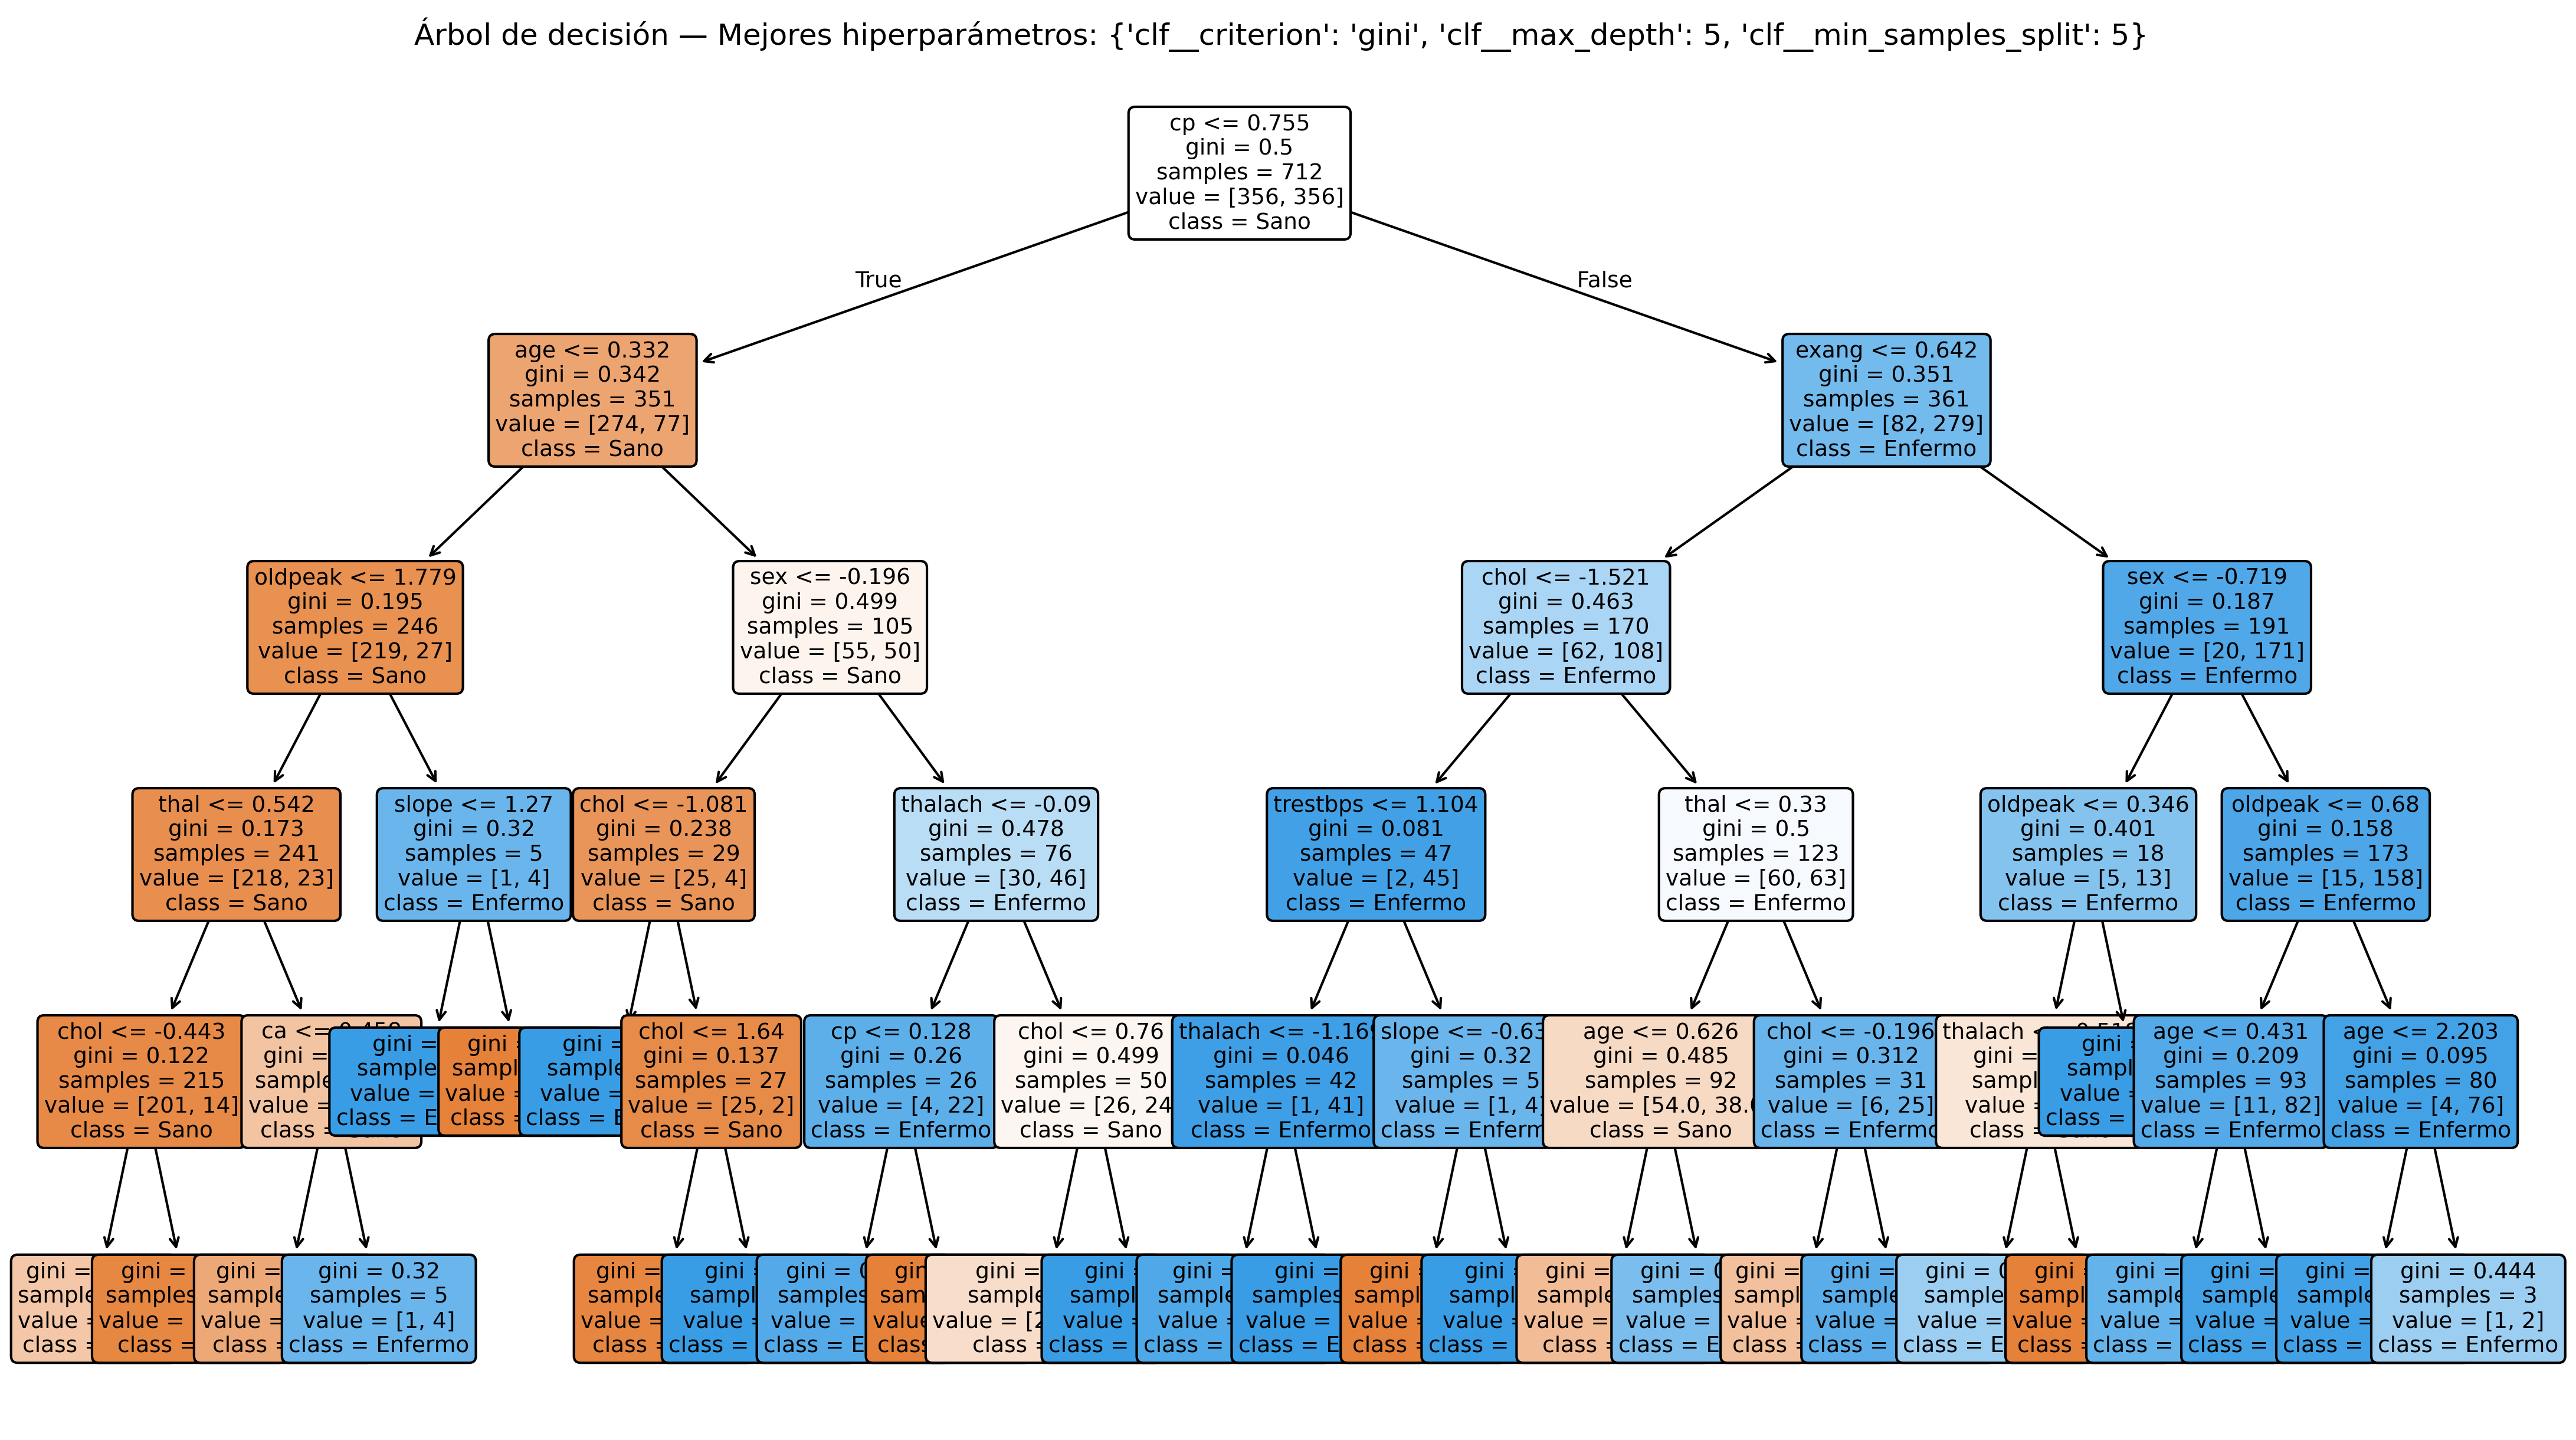
\includegraphics[width=1\textwidth]{Img/h_08_arbol_decision.png}
    \caption{Árbol de decisión entrenado sobre Heart Disease.}
    \label{fig:heart-arbol}
\end{figure}

\subsubsection*{Comparación e hiperparámetro más relevante}

La Figura~\ref{fig:heart-comparacion} muestra que la \textit{brecha}
entre CV y prueba es modesta para los tres modelos ($\sim 0.02$ en valor
absoluto), lo que sugiere que no hay sobreajuste significativo. El
patrón de hiperparámetros más relevantes
(Tabla~\ref{tab:heart-hiperparametros}) cambia respecto a Cancer:

\begin{figure}[H]
    \centering
    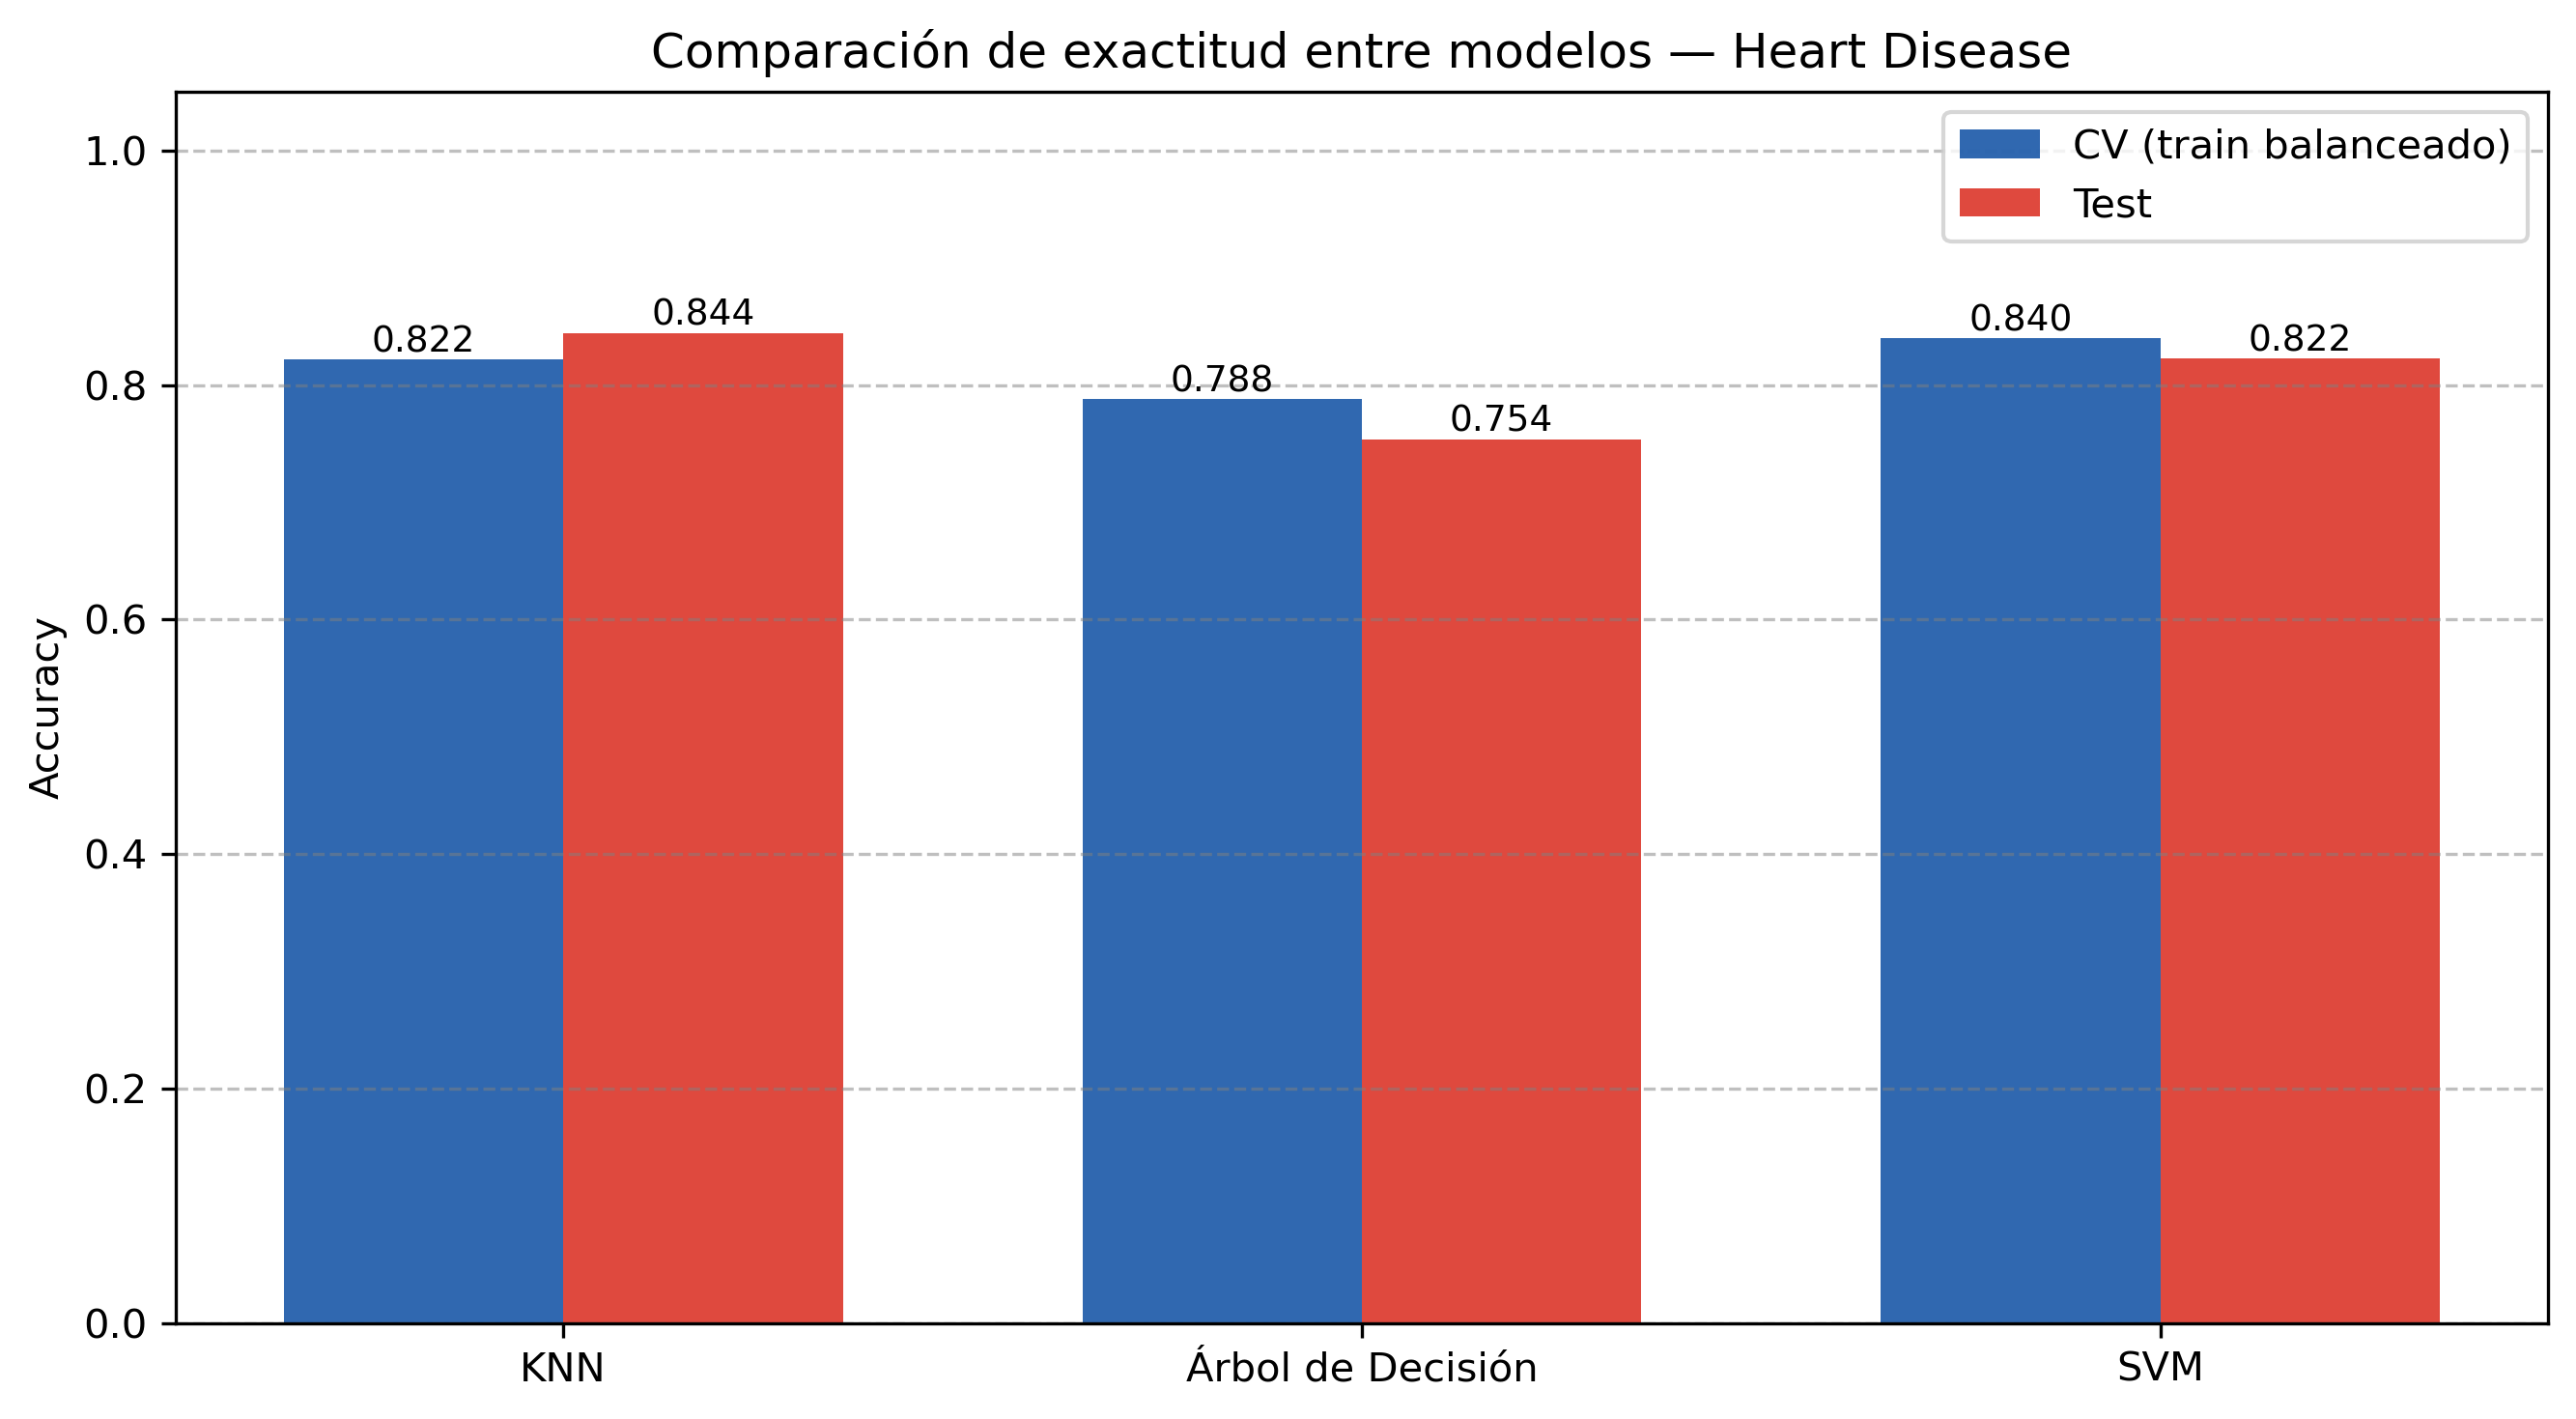
\includegraphics[width=0.85\textwidth]{Img/h_09_comparacion_exactitud.png}
    \caption{Comparación de exactitud CV vs Test sobre Heart Disease.}
    \label{fig:heart-comparacion}
\end{figure}

\begin{table}[H]
    \centering
    \rowcolors{2}{rowgray}{white}
    \begin{tabular}{lll}
        \toprule
        \rowcolor{headerblue}
        \textcolor{headertext}{\textbf{Modelo}}                       &
        \textcolor{headertext}{\textbf{Hiperparámetro más relevante}} &
        \textcolor{headertext}{\textbf{$\Delta$ accuracy}}                                               \\
        \midrule
        KNN                                                           & \texttt{n\_neighbors} & $0.0249$ \\
        Árbol de Decisión                                             & \texttt{max\_depth}   & $0.0161$ \\
        SVM                                                           & \texttt{C}            & $0.0096$ \\
        \bottomrule
    \end{tabular}
    \caption{Hiperparámetro más sensible por modelo sobre Heart Disease.}
    \label{tab:heart-hiperparametros}
\end{table}

En Heart Disease el \texttt{n\_neighbors} es el hiperparámetro más
relevante para KNN ($\Delta = 0.0249$, más del doble que en Cancer), lo
cual tiene sentido geométrico: cuando las clases se solapan, el tamaño
del vecindario determina si el modelo memoriza ruido ($k$ bajo) o
suaviza demasiado ($k$ alto). Para el árbol, la profundidad máxima toma
el protagonismo (frente al criterio en Cancer): con clases más mezcladas,
permitir más o menos divisiones cambia significativamente la complejidad
del modelo. El SVM mantiene a $C$ como hiperparámetro dominante en
ambos conjuntos, confirmando su rol estructural en la geometría del
margen.

\subsection{Comparación cruzada entre conjuntos}

La Tabla~\ref{tab:comparacion-final} sintetiza los mejores resultados de
los tres clasificadores sobre los dos conjuntos.

\begin{table}[H]
    \centering
    \rowcolors{2}{rowgray}{white}
    \begin{tabular}{lcccc}
        \toprule
        \rowcolor{headerblue}
        \textcolor{headertext}{\textbf{Modelo}}           &
        \textcolor{headertext}{\textbf{Cancer Test Acc.}} &
        \textcolor{headertext}{\textbf{Cancer Test F1}}   &
        \textcolor{headertext}{\textbf{Heart Test Acc.}}  &
        \textcolor{headertext}{\textbf{Heart Test F1}}                                                                                    \\
        \midrule
        KNN                                               & $0.9532$          & $0.9394$          & $\mathbf{0.8442}$ & $\mathbf{0.8599}$ \\
        Árbol de Decisión                                 & $0.9474$          & $0.9302$          & $0.7536$          & $0.7671$          \\
        SVM                                               & $\mathbf{0.9766}$ & $\mathbf{0.9692}$ & $0.8225$          & $0.8444$          \\
        \bottomrule
    \end{tabular}
    \caption{Comparación cruzada de los mejores modelos en los dos
        conjuntos de datos.}
    \label{tab:comparacion-final}
\end{table}

Tres lecturas se desprenden de la comparación:

\begin{enumerate}
    \item \textbf{La dificultad del problema gobierna el techo, no el modelo.}
          La caída de $\sim 0.13$ puntos en exactitud al pasar de Cancer a
          Heart Disease es transversal a los tres clasificadores y refleja
          la separabilidad inherente al espacio de características. En
          Cancer las dos primeras componentes principales casi separan
          linealmente las clases; en Heart Disease incluso 12 componentes
          dejan zonas de mezcla considerables.

    \item \textbf{El SVM domina cuando hay margen claro.} En Cancer, donde
          las clases admiten una separación casi lineal en alta dimensión,
          el SVM lineal ofrece el mejor compromiso entre simplicidad y
          desempeño. En Heart Disease, donde la frontera es más compleja y
          la dimensión efectiva es prácticamente la original, el SVM con
          kernel RBF mantiene la cabeza pero pierde el liderato frente al
          KNN, que se beneficia de las relaciones locales entre vecinos
          tras el sobremuestreo de SMOTE.

    \item \textbf{El árbol es siempre la opción menos competitiva.} Un único
          árbol carece de la flexibilidad de los \textit{ensembles}
          (Random Forest, Gradient Boosting) y compite en desventaja
          incluso cuando los datos son fáciles. Su valor real está en la
          interpretabilidad ---el camino raíz-hoja es una regla diagnóstica
          legible--- más que en la exactitud bruta.
\end{enumerate}
